%%%%%%%%%%%%%%%%%%%%%%%%%%%%%%%%%%%%%%%%%
% kaobook
% LaTeX Template
% Version 1.2 (4/1/2020)
%
% This template originates from:
% https://www.LaTeXTemplates.com
%
% For the latest template development version and to make contributions:
% https://github.com/fmarotta/kaobook
%
% Authors:
% Federico Marotta (federicomarotta@mail.com)
% Based on the doctoral thesis of Ken Arroyo Ohori (https://3d.bk.tudelft.nl/ken/en)
% and on the Tufte-LaTeX class.
% Modified for LaTeX Templates by Vel (vel@latextemplates.com)
%
% License:
% CC0 1.0 Universal (see included MANIFEST.md file)
%
%%%%%%%%%%%%%%%%%%%%%%%%%%%%%%%%%%%%%%%%%

%----------------------------------------------------------------------------------------
%	PACKAGES AND OTHER DOCUMENT CONFIGURATIONS
%----------------------------------------------------------------------------------------

\documentclass[
    a4paper, % Page size
    fontsize=10pt, % Base font size
    twoside=true, % Use different layouts for even and odd pages (in particular, if twoside=true, the margin column will be always on the outside)
	%open=any, % If twoside=true, uncomment this to force new chapters to start on any page, not only on right (odd) pages
	%chapterentrydots=true, % Uncomment to output dots from the chapter name to the page number in the table of contents
	numbers=noenddot, % Comment to output dots after chapter numbers; the most common values for this option are: enddot, noenddot and auto (see the KOMAScript documentation for an in-depth explanation)
]{kaobook}

% Set the language
\usepackage[english]{babel} % Load characters and hyphenation
\usepackage[english=british]{csquotes} % English quotes

% Load packages for testing
\usepackage{blindtext}
%\usepackage{showframe} % Uncomment to show boxes around the text area, margin, header and footer
%\usepackage{showlabels} % Uncomment to output the content of \label commands to the document where they are used
\usepackage{graphicx}
\usepackage[percent]{overpic}
\usepackage[utf8]{inputenc}
% \usepackage{natbib}
\usepackage{amsmath}
\usepackage{siunitx}
\sisetup{group-separator = {,}}
\usepackage{subcaption}
\usepackage{todonotes}
\usepackage[version=4]{mhchem}
\usepackage{wasysym}
\usepackage{overpic}
\usepackage[dvipsnames]{xcolor}

\definecolor{yellow}{RGB}{180, 95, 6}
\definecolor{grey}{RGB}{183, 183, 183}
\definecolor{orange}{RGB}{228, 146, 64}

\newcolumntype{L}[1]{>{\raggedright\arraybackslash}p{#1}}
\newcolumntype{C}[1]{>{\centering\arraybackslash}p{#1}}
\newcolumntype{R}[1]{>{\raggedleft\arraybackslash}p{#1}}
\newcommand\cruleme[3][black]{\textcolor{#1}{\rule{#2}{#3}}}

% Load the bibliography package
\usepackage{kaobiblio}
\addbibresource{main.bib} % Bibliography file

\RenewDocumentCommand{\formatmargincitation}{m}{
	\parencite{#1} \citeauthor*{#1} (\citeyear{#1})\\
}

% Load mathematical packages for theorems and related environments
\usepackage[framed=true]{kaotheorems}

% Load the package for hyperreferences
\usepackage{kaorefs}

\graphicspath{{examples/documentation/images/}{images/}} % Paths in which to look for images

\makeindex[columns=3, title=Alphabetical Index, intoc] % Make LaTeX produce the files required to compile the index

\makeglossaries % Make LaTeX produce the files required to compile the glossary
\newglossaryentry{monoblock}{
	name=monoblock,
	description={A unit brick made of a tungsten armour with a CuCrZr cooling pipe and a copper interlayer},
}
\newglossaryentry{plasma}{
	name=plasma,
	description={Ionised gas. Sometimes refered as the fourth state of matter}
}
\newglossaryentry{divertor}{
	name=divertor,
	description={Component of a tokamak diverting the magnetic field lines creating one or several X-points. The divertor is responsible for exhausting heat and particle from the plasma. The targets of the divertor is where the plasma is directed to absorb heat and particle fluxes},
}
\newglossaryentry{strike point}{
	name=strike point,
	description={Location on the divertor where the serparatrix crosses the solid target. It is where the highest heat and particle fluxes are observed},
}
\newglossaryentry{x-point}{
	name=X-point,
	description={Point in space where the poloidal field has zero magnitude},
}
\newglossaryentry{separatrix}{
	name=separatrix,
	description={Last closed flux surface, intersects the X-point},
}
\newglossaryentry{private flux region}{
	name=private flux region,
	description={WEST divertor region located between the strike points}
}
\newglossaryentry{fuel recycling}{
	name=fuel recycling,
	description={Phenomenon occuring when particles from the plasma are neutralised at the walls and ionised again}
}
\newglossaryentry{breeding blanket}{
	name=breeding blanket,
	description={Components of a fusion reactor responsible for producing tritium from the neutrons of the fusion reactions},
}
\newglossaryentry{first wall}{
	name=first wall,
	description={Cover of the inner surface of the vacuum vessel in front of the plasma},
}

\newglossaryentry{isotope}{
	name=isotope,
	description={Member of a family of elements sharing the same number of protons but different numbers of neutrons}
}
\newglossaryentry{transmutation}{
	name=transmutation,
	description={Conversion of a chemical element into another chemical element by changing the number of neutrons or protons in the nucleus}
}
\newglossaryentry{transmutation gas}{
	name=transmutation gas,
	description={Gas produced by transmutation (typically helium or hydrogen)}
}

\newglossaryentry{diffusion}{
	name=diffusion,
	description={For particles: process resulting from the random motion of particles from high concentration regions to regions of low concentrations. For heat: transport of thermal energy from high temperature regions to low temperature regions}
}
\newglossaryentry{permeation}{
	name=permeation,
	description={Transport of particles through a material membrane}
}
\newglossaryentry{advection}{
	name=advection,
	description={Transport of particles (or heat) via motion of the medium (as opposed to diffusion where the medium can be immobile)}
}
\newglossaryentry{trapping}{
	name=trapping,
	description={Process involving a particle being retained in a potential energy well}
}
\newglossaryentry{detrapping}{
	name=detrapping,
	description={Opposite to trapping}
}
\newglossaryentry{Soret effect}{
	name=Soret effect,
	description={Diffusion assisted by thermal gradients}
}
\newglossaryentry{thermophoresis}{
	name=thermophoresis,
	description={See Soret effect}
}


\newglossaryentry{dislocation loop}{
	name=dislocation loop,
	description={Defects formed by agglomerations of point-defects into planes}
}
\newglossaryentry{self-interstitial}{
	name=self-interstitial,
	description={An atom initially in the lattice located at interstitial sites}
}
\newglossaryentry{vacancy}{
	name=vacancy,
	description={Defect in the lattice where a metal atom is missing},
	plural=vacancies
}
\newglossaryentry{Frenkel pair}{
	name=Frenkel pair,
	description={A self-interstitial atom and a vacancy}
}
\newglossaryentry{trap mutation}{
	name=trap mutation,
	description={Process where over-pressurised helium clusters eject a metal lattice atom creating a Frenkel pair}
}
\newglossaryentry{self-trapping}{
	name=self-trapping,
	description={See trap mutation entry}
}

\newglossaryentry{loop punching}{
	name=loop punching,
	description={Helium bubble growth mechanism leading to the formation of a dislocation loop}
}
\newglossaryentry{fuzz}{
	name=fuzz,
	description={Porous, nanostructure sometimes observed on tungsten under helium irradiation}
}
\newglossaryentry{tendril}{
	name=tendril,
	description={Nanometre-thick columns forming the fuzz}
}
\newglossaryentry{blistering}{
	name=blistering,
	description={Formation of blisters: plastic deformation (swelling) of the metal near the surface due to high pressure in bubbles}
}
\newglossaryentry{bursting}{
	name=bursting,
	description={Explosion of a gas bubble near the metal surface}
}


\newglossaryentry{fluence}{
	name=fluence,
	description={Total quantitiy of particles a sample has been exposed to over a given period of time. Product of the particle flux by the exposure time}
}
\newglossaryentry{retention}{
	name=retention,
	description={Local concentration of soluted species (hydrogen or helium) including the mobile species and the trapped ones}
}
\newglossaryentry{inventory}{
	name=inventory,
	description={Total quantity of particles in a domain (sample, component, reactor...). It can be obtained by integrating the retention over the domain}
}
\newglossaryentry{startup inventory}{
	name=startup inventory,
	description={Tritium inventory required by new reactors to account for the initial tritium losses (processing time, trapping in components...)}
}

% Glossary entries (used in text with e.g. \acrfull{fpsLabel} or \acrshort{fpsLabel})
\newacronym{H}{H}{Hydrogen}
\newacronym{He}{He}{Helium}
\newacronym{D}{D}{Deuterium}
\newacronym{T}{T}{Tritium}
\newacronym{Li}{Li}{Lithium}
\newacronym{W}{W}{Tungsten}


\newacronym[longplural={Plasma Facing Units}, shortplural={PFUs}]{pfuLabel}{PFU}{Plasma Facing Unit}
\newacronym[longplural={Plasma Facing Materials}, shortplural={PFMs}]{pfm}{PFM}{Plasma Facing Material}
\newacronym{cfc}{CFC}{Carbon fiber composite}
\newacronym{ivt}{IVT}{Inner Vertical Target}
\newacronym{ovt}{OVT}{Outer Vertical Target}
\newacronym{isp}{ISP}{Inner Strike Point}
\newacronym{osp}{OSP}{Outer Strike Point}

\newacronym{hcpb}{HCPB}{Helium-Cooled-Pebble-Bed}
\newacronym{wcll}{WCLL}{Water-Cooled-Lithium-Lead}
\newacronym{hcll}{HCLL}{Helium-Cooled-Liquid-Lead}
\newacronym{dcll}{DCLL}{Dual-Coolant-Lithium-Lead}
\newacronym{tbr}{TBR}{Tritium breeding ratio}
\newacronym{fpy}{FPY}{Full power year}


\newglossaryentry{tokamak}{
	name=tokamak,
	description={Toroidal fusion reactor using magnetic fields to confine the plasma. Acronym for "TOroidalnaïa KAmera s MAgnitnymi Katouchkami", which means "Toroidal chamber with magnetic coils"}
}
\newglossaryentry{stellarator}{
	name=stellarator,
	description={Toroidal fusion reactor using magnetic fields to confine the plasma. The difference with the tokamak is the twisted magnetic coils and the absence of a central solenoid inducing a current in the plasma}
}
\newacronym{candu}{CANDU}{CANada Deuterium Uranium reactor}
\newacronym{west}{WEST}{Tungsten Environment Steady state Tokamak}
\newacronym{jet}{JET}{Joint European Torus}
\newacronym{iter}{ITER}{International Thermonuclear Experimental Reactor}
\newacronym{demo}{DEMO}{DEMOnstration power plant}
\newacronym{sparc}{SPARC}{Soonest Private-funded Affordable Robust Compact}
\newacronym{arc}{ARC}{Affordable Robust Compact}
\newacronym{nif}{NIF}{National Ignition Facility}
\newacronym{mast-u}{MAST-U}{Mega Amp Spherical Tokamak Ugrade}
\newacronym{step}{STEP}{Spherical Tokamak for Electricity Production}
\newacronym{ukaea}{UKAEA}{United-Kingdom Atomic Energy Authority}

\newacronym{md}{MD}{Molecular Dynamics}
\newacronym{dft}{DFT}{Density Functional Theory}
\newacronym{eels}{EELS}{Electron Energy Loss Spectroscopy}
\newacronym{tds}{TDS}{Themo-Desorption Spectroscopy}
\newacronym{tem}{TEM}{Transmission Electron Microscopy}
\newacronym{mms}{MMS}{Method of Manufactured Solutions}
\newacronym{mes}{MES}{Method of Exact Solutions}
\newacronym{mre}{MRE}{Macroscopic Rate Equations}
\newacronym{vv}{V\&V}{Verification and Validation}
\newglossaryentry{p1}{
	name=P1,
	description={Lagrange finite element of order 1, also called piecewise linear elements.}
}
\newglossaryentry{p2}{
	name=P2,
	description={Lagrange finite element of order 2.}
}
\newglossaryentry{p3}{
	name=P3,
	description={Lagrange finite element of order 3.}
}
\newacronym{bcc}{bcc}{Body-Centered Cubic (type of metallic lattice)}
\newglossaryentry{lattice}{
	name=Lattice,
	description={Three-dimensional crystalline structure of metals. The lattice is how the atoms are ordered within a metal}
}

\newacronym{fdm}{FDM}{Finite Difference Method}
\newacronym{fem}{FEM}{Finite Element Method}
\newacronym{festim}{FESTIM}{Finite Element Simulation of Tritium in Materials}
\newacronym{tmap7}{TMAP7}{Tritium Migration Analysis Program, Version 7}
\newacronym{hiipc}{HIIPC}{Hydrogen Isotope Inventory Processes Code}
\newacronym{crds}{CRDS}{Coupled Reaction Diffusion System}
\newacronym{mhims}{MHIMS}{Migration of Hydrogen Isotopes in MaterialS}
\newacronym{tessim}{TESSIM}{Tritium Extraction System SIMulator}
\newacronym{hit}{HIT}{Hydrogen Isotope Transport code}
\newglossaryentry{achlys}{
	name=ACHLYS,
	description={Hydrogen transport code developed by UKAEA}
}
\newglossaryentry{paramak}{
	name=Paramak,
	description={Code for generating parametric tokamak geometries}
}
\newglossaryentry{openmc}{
	name=OpenMC,
	description={Open-source neutronics code}
}
\newglossaryentry{fenics}{
	name=FEniCS,
	description={Open-source finite element solving library}
}
\newacronym{imas}{IMAS}{Integrated Modelling Analysis Suite}
\newacronym{srim}{SRIM}{Stopping Range of Ions in Matter}
\newglossaryentry{solps}{
	name=SOLPS-ITER,
	description={Primary plasma boundary code used at ITER}
}
\newglossaryentry{soledge}{
	name=SOLEDGE3X,
	description={Plasma boundary code}
}

\newacronym{cg}{CG}{Conjugate Gradient}
\newacronym{tnc}{TNC}{Truncated Newton method}

 % Include the glossary definitions

\makenomenclature % Make LaTeX produce the files required to compile the nomenclature

% Reset sidenote counter at chapters
%\counterwithin*{sidenote}{chapter}

%----------------------------------------------------------------------------------------

\begin{document}

%----------------------------------------------------------------------------------------
%	BOOK INFORMATION
%----------------------------------------------------------------------------------------
\titlehead{The \texttt{kaobook} class}
\subject{Use this document as a template}

\title[Example and documentation of the {\normalfont\texttt{kaobook}} class]{Example and documentation \\ of the {\normalfont\texttt{kaobook}} class}
\subtitle{Customise this page according to your needs}

\author[Federico Marotta]{Federico Marotta \thanks{A \LaTeX\ lover}}

\date{\today}

\publishers{An Awesome Publisher}

%----------------------------------------------------------------------------------------

\frontmatter % Denotes the start of the pre-document content, uses roman numerals

%----------------------------------------------------------------------------------------
%	OPENING PAGE
%----------------------------------------------------------------------------------------

%\makeatletter
%\extratitle{
%	% In the title page, the title is vspaced by 9.5\baselineskip
%	\vspace*{9\baselineskip}
%	\vspace*{\parskip}
%	\begin{center}
%		% In the title page, \huge is set after the komafont for title
%		\usekomafont{title}\huge\@title
%	\end{center}
%}
%\makeatother

%----------------------------------------------------------------------------------------
%	COPYRIGHT PAGE
%----------------------------------------------------------------------------------------

\makeatletter
\uppertitleback{\@titlehead} % Header

\lowertitleback{
	\textbf{Disclaimer}\\
	You can edit this page to suit your needs. For instance, here we have a no copyright statement, a colophon and some other information. This page is based on the corresponding page of Ken Arroyo Ohori's thesis, with minimal changes.
	
	\medskip
	
	\textbf{No copyright}\\
	\cczero\ This book is released into the public domain using the CC0 code. To the extent possible under law, I waive all copyright and related or neighbouring rights to this work.
	
	To view a copy of the CC0 code, visit: \\\url{http://creativecommons.org/publicdomain/zero/1.0/}
	
	\medskip
	
	\textbf{Colophon} \\
	This document was typeset with the help of \href{https://sourceforge.net/projects/koma-script/}{\KOMAScript} and \href{https://www.latex-project.org/}{\LaTeX} using the \href{https://github.com/fmarotta/kaobook/}{kaobook} class.
	
	The source code of this book is available at:\\\url{https://github.com/fmarotta/kaobook}
	
	(You are welcome to contribute!)
	
	\medskip
	
	\textbf{Publisher} \\
	First printed in May 2019 by \@publishers
}
\makeatother

%----------------------------------------------------------------------------------------
%	DEDICATION
%----------------------------------------------------------------------------------------

\dedication{
	The harmony of the world is made manifest in Form and Number, and the heart and soul and all the poetry of Natural Philosophy are embodied in the concept of mathematical beauty.\\
	\flushright -- D'Arcy Wentworth Thompson
}

%----------------------------------------------------------------------------------------
%	OUTPUT TITLE PAGE AND PREVIOUS
%----------------------------------------------------------------------------------------

% Note that \maketitle outputs the pages before here

% If twoside=false, \uppertitleback and \lowertitleback are not printed
% To overcome this issue, we set twoside=semi just before printing the title pages, and set it back to false just after the title pages
\KOMAoptions{twoside=semi}
\maketitle
\KOMAoptions{twoside=false}

%----------------------------------------------------------------------------------------
%	PREFACE
%----------------------------------------------------------------------------------------

\chapter*{Preface}
\addcontentsline{toc}{chapter}{Preface} % Add the preface to the table of contents as a chapter

I am of the opinion that every \LaTeX\xspace geek, at least once during 
his life, feels the need to create his or her own class: this is what 
happened to me and here is the result, which, however, should be seen as 
a work still in progress. Actually, this class is not completely 
original, but it is a blend of all the best ideas that I have found in a 
number of guides, tutorials, blogs and tex.stackexchange.com posts. In 
particular, the main ideas come from two sources:

\begin{itemize}
	\item \href{https://3d.bk.tudelft.nl/ken/en/}{Ken Arroyo Ohori}'s 
	\href{https://3d.bk.tudelft.nl/ken/en/nl/ken/en/2016/04/17/a-1.5-column-layout-in-latex.html}{Doctoral 
	Thesis}, which served, with the author's permission, as a backbone 
	for the implementation of this class;
	\item The 
		\href{https://github.com/Tufte-LaTeX/tufte-latex}{Tufte-Latex 
			Class}, which was a model for the style.
\end{itemize}

The first chapter of this book is introductive and covers the most 
essential features of the class. Next, there is a bunch of chapters 
devoted to all the commands and environments that you may use in writing 
a book; in particular, it will be explained how to add notes, figures 
and tables, and references. The second part deals with the page layout 
and design, as well as additional features like coloured boxes and 
theorem environments.

I started writing this class as an experiment, and as such it should be 
regarded. Since it has always been indended for my personal use, it may 
not be perfect but I find it quite satisfactory for the use I want to 
make of it. I share this work in the hope that someone might find here 
the inspiration for writing his or her own class.

\begin{flushright}
	\textit{Federico Marotta}
\end{flushright}


%----------------------------------------------------------------------------------------
%	TABLE OF CONTENTS & LIST OF FIGURES/TABLES
%----------------------------------------------------------------------------------------

\begingroup % Local scope for the following commands

% Define the style for the TOC, LOF, and LOT
%\setstretch{1} % Uncomment to modify line spacing in the ToC
%\hypersetup{linkcolor=blue} % Uncomment to set the colour of links in the ToC
\setlength{\textheight}{23cm} % Manually adjust the height of the ToC pages

% Turn on compatibility mode for the etoc package
\etocstandarddisplaystyle % "toc display" as if etoc was not loaded
\etocstandardlines % toc lines as if etoc was not loaded

\tableofcontents % Output the table of contents

\listoffigures % Output the list of figures

% Comment both of the following lines to have the LOF and the LOT on different pages
\let\cleardoublepage\bigskip
\let\clearpage\bigskip

\listoftables % Output the list of tables

\endgroup

%----------------------------------------------------------------------------------------
%	MAIN BODY
%----------------------------------------------------------------------------------------

\mainmatter % Denotes the start of the main document content, resets page numbering and uses arabic numbers
\setchapterstyle{kao} % Choose the default chapter heading style

% Chapter 1
\setchapterimage{jet}
\setchapterpreamble[u]{\margintoc}
\chapter{Fusion: general introduction} % Main chapter title
\label{Chapter1} % For referencing the chapter elsewhere, use \ref{Chapter1} 
\section{Thermonuclear fusion: principles}
\subsection{Tokamaks: how to put the sun in a bottle}
\subsection{Main challenges}
\section{Plasma-surface interactions in tokamaks}
\subsection{H/W, He/W and He/H interactions}
\subsection{Experimental methods}
\subsection{Modelling methods}
\section{Roadmap}





% \pagelayout{wide} % No margins
% \addpart{Class Options, Commands and Environments}
% \pagelayout{margin} % Restore margins

% \setchapterstyle{kao}
%\setchapterpreamble[u]{\margintoc}
\chapter{References}
\labch{references}

\section{Citations}

\index{citations}
To cite someone \sidecite{Visscher2008,James2013} is very simple: just 
use the \Command{sidecite}\index{\Command{sidecite}} command. It does 
not have an offset argument yet, but it probably will in the future. 
This command supports multiple entries, as you can see, and by default 
it prints the reference on the margin as well as adding it to the 
bibliography at the end of the document. Note that the citations have 
nothing to do with the text,\sidecite{James2013} but they are completely 
random as they only serve the purpose to illustrate the feature.

For this setup I wrote a separate package, \Package{kaobiblio}, which 
you can find in the \Package{styles} directory and include in your main 
tex file. This package accepts all the options that you can pass to 
\Package{biblatex}, and actually it passes them to \Package{biblatex} 
under the hood. Moreover, it also defines some commands, like 
\Command{sidecite}, and environments that can be used within a 
\Class{kao} book.\sidenote{For this reason you should always use 
\Package{kaobiblio} instead of \Package{biblatex}, but the syntax and 
the options are exactly the same.}

As you have seen, the \Command{sidecite} command will print a citation 
in the margin. However, this command would be useless without a way to 
customise the format of the citation, so the \Class{kaobook} provides 
also the \Command{formatmargincitation} command. By \enquote{renewing} 
that command, you can choose which items will be printed in the margins. 
The best way to understand how it works is to see the actual definition 
of this command.

\begin{lstlisting}[style=kaolstplain,linewidth=1.5\textwidth]
\newcommand{\formatmargincitation}[1]{
	\parencite{#1}: \citeauthor*{#1} (\citeyear{#1}), \citetitle{#1}\\
}
\end{lstlisting}

Thus, the \Command{formatmargincitation} accepts one parameter, which is 
the citation key, and prints the parencite followed by a colon, then the 
author, then the year (in brackets), and finally the 
title.\sidecite{Battle2014} Now, suppose that you wish the margin 
citation to display the year and the author, followed by the title, and 
finally a fixed arbitrary string; you would add to your document:

\begin{lstlisting}[style=kaolstplain,linewidth=1.5\textwidth]
\renewcommand{\formatmargincitation}[1]{
	\citeyear{#1}, \citeauthor*{#1}: \citetitle{#1}; very interesting!\\
}
\end{lstlisting}

\renewcommand{\formatmargincitation}[1]{
	\citeyear{#1}, \citeauthor*{#1}: \citetitle{#1}; very interesting!\\
}

The above code results in citations that look like the 
following.\sidecite{Zou2005} Of course, changing the format is most 
useful when you also change the default bibliography style. For 
instance, if you want to use the \enquote{philosophy-modern} style for 
your bibliography, you might have something like this in the preamble:

\begin{lstlisting}[style=kaolstplain,linewidth=1.5\textwidth]
\usepackage[style=philosophy-modern]{styles/kaobiblio}
\renewcommand{\formatmargincitation}[1]{
	\sdcite{#1}\\
}
\addbibresource{main.bib}
\end{lstlisting}

\renewcommand{\formatmargincitation}[1]{
	\parencite{#1}: \citeauthor*{#1} (\citeyear{#1}), \citetitle{#1}\\
}

The commands like \Command{citeyear}, \Command{parencite} and 
\Command{sdcite} are just examples. A full reference of the available 
commands can be found in this 
\href{http://tug.ctan.org/info/biblatex-cheatsheet/biblatex-cheatsheet.pdf}{cheatsheet}, 
under the \enquote{Citations} section.

Finally, to compile a document containing citations, you need to use an 
external tool, which for this class is biber. You need to run the 
following (assuming that your tex file is called main.tex):

\begin{lstlisting}[style=kaolstplain]
$ pdflatex main
$ biber main
$ pdflatex main
\end{lstlisting}

\section{Glossaries and Indices}

\index{glossary}
The \Class{kaobook} class loads the packages \Package{glossaries} and 
\Package{imakeidx}, with which you can add glossaries and indices to 
your book. For instance, I previously defined some glossary entries and 
now I am going to use them, like this: \gls{computer}. 
\Package{glossaries} also allows you to use acronyms, like the 
following: this is the full version, \acrfull{fpsLabel}, and this is the 
short one \acrshort{fpsLabel}. These entries will appear in the glossary 
in the backmatter.

Unless you use \href{https://www.overleaf.com}{Overleaf} or some other 
fancy IDE for \LaTeX, you need to run an external command from your 
terminal in order to compile a document with a glossary. In particular, 
the commands required are:\sidenote{These are the commands you 
would run in a UNIX system; I have no idea on how it works in Windows.}

\begin{lstlisting}[style=kaolstplain]
$ pdflatex main
$ makeglossaries main
$ pdflatex main
\end{lstlisting}

Note that you need not run \texttt{makeglossaries} every time you 
compile your document, but only when you change the glossary entries.

\index{index}
To create an index, you need to insert the command 
\lstinline|\index{subject}| whenever you are talking about 
\enquote{subject} in the text. For instance, at the start of this 
paragraph I would write \lstinline|index{index}|, and an entry would be 
added to the Index in the backmatter. Check it out!

\marginnote[2mm]{In theory, you would need to run an external command 
for the index as well, but luckily the package we suggested, 
	\Package{imakeidx}, can compile the index automatically.}

\index{nomenclature}
A nomenclature is just a special kind of index; you can find one at the end of
this book. To insert a nomenclature, we use the package \Package{nomencl} and
add the terms with the command \Command{nomenclature}. We put then a
\Command{printnomenclature} where we want it to appear.

Also with this package we need to run an external command to compile the 
document, otherwise the nomenclature will not appear:

\begin{lstlisting}[style=kaolstplain]
$ pdflatex main
$ makeindex main.nlo -s nomencl.ist -o main.nls
$ pdflatex main
\end{lstlisting}

These packages are all loaded in 
\href{style/packages.sty}{packages.sty}, one of the files that come with 
this class. However, the configuration of the elements is best done in 
the main.tex file, since each book will have different entries and 
styles.

Note that the \Package{nomencl} package caused problems when the 
document was compiled, so, to make a long story short, I had to prevent 
\Package{scrhack} to load the hack-file for \Package{nomencl}. When 
compiling the document on Overleaf, however, this problem seem to 
vanish.

\marginnote[-19mm]{This brief section was by no means a complete 
reference on the subject, therefore you should consult the documentation 
of the above package to gain a full understanding of how they work.}

\section{Hyperreferences}
\labsec{hyprefs}

\index{hyperreferences}
In this class we provide a handy sub-package to help you referencing the 
same elements always in the same way, for consistency across the book. 
First, you can label each element with a specific command. For instance, 
should you want to label a chapter, you would put 
\lstinline|\labch{chapter-title}| right after the \Command{chapter} 
directive. This is just a convienence, because \Command{labch} is 
actually just an alias to \lstinline|\label{ch:chapter-title}|, so it 
spares you the writing of \enquote{ch}. We defined similar commands for 
many typically labeled elements, including:

\begin{multicols}{2}
\setlength{\columnseprule}{0pt}
\begin{itemize}
	\item Page: \Command{labpage}
	\item Part: \Command{labpart}
	\item Chapter: \Command{labch}
	\item Section: \Command{labsec}
	\item Figure: \Command{labfig}
	\item Table: \Command{labtab}
	\item Definition: \Command{labdef}
	\item Theorem: \Command{labthm}
	\item Proposition: \Command{labprop}
	\item Lemma: \Command{lablemma}
	\item Remark: \Command{labremark}
	\item Example: \Command{labexample}
	\item Exercise: \Command{labexercise}
\end{itemize}
\end{multicols}

Of course, we have similar commands for referencing those elements. 
However, since the style of the reference should depend on the context, 
we provide different commands to reference the same thing. For instance, 
in some occasions you may want to reference the chapter by name, but 
other times you want to reference it only by number. In general, there 
are four reference style, which we call plain, vario, name, and full. 

The plain style references only by number. It is accessed, for chapters, 
with \lstinline|\refch{chapter-title}| (for other elements, the syntax 
is analogous). Such a reference results in: \refch{references}.

The vario and name styles rest upon the \Package{varioref} package. 
Their syntax is \lstinline|\vrefch{chapter-title}| and 
\lstinline|\nrefch{chapter-title}|, and they result in: 
\vrefch{references}, for the vario style, and: \nrefch{references}, for 
the name style. As you can see, the page is referenced in 
\Package{varioref} style.

The full style references everything. You can use it with 
\lstinline|\frefch{chapter-title}| and it looks like this: 
\frefch{references}.

Of course, all the other elements have similar commands (\eg for parts 
you would use \lstinline|\vrefpart{part-title}| or something like that). 
However, not all elements implement all the four styles. The commands 
provided should be enough, but if you want to see what is available or 
to add the missing ones, have a look at the 
\href{styles/kaorefs.sty}{attached package}.


% \pagelayout{wide} % No margins
% \addpart{Design and Additional Features}
% \pagelayout{margin} % Restore margins

% \input{chapters/layout.tex}
% \input{chapters/mathematics.tex}

% \setchapterimage[3cm]{seaside}
\chapter{Model description}
\label{Chapter2} % For referencing the chapter elsewhere, use \ref{Chapter2} 
\section{Introduction}
\section{H transport} \label{description_H_transport_model}
\subsection{Bulk model}
As in most of MRE models, HIs are split in several populations which are the mobile and the trapped ones in the i-th trap, described using their concentration (respectively $c_\mathrm{m}$ and $c_{\mathrm{t},i}$).
The spatio temporal evolution of these concentrations are commonly described by the following reaction-diffusion system:

\begin{equation}
    \frac{\partial c_\mathrm{m}}{\partial t}=\vec{\nabla} \cdot\left(D(T) \vec{\nabla}c_\mathrm{m}\right)+\Gamma-\sum \frac{\partial c_{\mathrm{t}, i}}{\partial t}
    \label{eq:mobile}
\end{equation}

\begin{equation}
    \frac{\partial c_{\mathrm{t}, i}}{\partial t}=k(T) \cdot c_\mathrm{m} \cdot\left(n_{i}-c_{\mathrm{t}, i}\right)-p(T) \cdot c_{\mathrm{t}, i}
    \label{eq:trapped}
\end{equation}

In Equation \ref{eq:mobile}, ${D(T)=D_0 \exp\big(\frac{-E_\mathrm{D}}{k_B \cdot T}\big)}$ is the diffusion coefficient in \si{m^2.s^{-1}}, $T$ being the temperature in $\si{K}$ and ${k_B = 8.617 \times 10^{-5} \si{eV.K^{-1}}}$ the Boltzmann constant, $\Gamma$ is the volumetric source term of particles in \si{m^{-3}.s^{-1}}, $k(T)=k_0\exp{\big(\frac{-E_{k, i}}{k_B \cdot T}\big)}$ and $p(T)=p_0\exp{\big(\frac{-E_{p, i}}{k_B \cdot T}\big)}$ are the trapping and detrapping rates expressed in \si{m^3.s^{-1}} and \si{s^{-1}} respectively and $n_i$ is the trap density in \si{m^{-3}}.
The unit of the different concentration, $c_\mathrm{m}$ and $c_{\mathrm{t},i}$ are in $ \si{m^{-3}}$ but can be expressed in atomic fraction (at.fr.) by normalising them to the atomic density of the material.

% maybe write something about the soret effect

\subsection{Boundary conditions}

Several boundary conditions will be employed in order to constrain either the actual solution (Dirichlet) or the solution gradient (Neumann, Robin) at the domain's boundaries.

\subsubsection{Imposed concentration}

Concentration can be fixed at the surface by applying Dirichlet boundary conditions as described in Equation \ref{eq:dirichlet bc}.
\begin{equation}
    c_\mathrm{m} = c_0(x, t) \quad \text { on } \partial \Omega
    \label{eq:dirichlet bc}
\end{equation}
where $\partial \Omega$ is the domain boundary.

$c_0$ can be calculated from Sievert's law of equilibrium and Equation \ref{eq:dirichlet bc} reads:
\begin{equation}
    c_\mathrm{m} = S(T) \sqrt{P}\quad \text { on } \partial \Omega
\end{equation}
where $P$ is the partial pressure of hydrogen at the boundary in \si{Pa}, $S(T)=S_0 \exp(\frac{-E_S}{k_B T})$ is the material solubility in \si{m^{-3}.Pa^{-1/2}} and $T$ is the local temperature in \si{K}.
This law of equilibrium is a steady-state approximation of a more complex model which takes into account flux exchanges between adsorbed and mobile concentrations at the boundary.
It is therefore valid when applied to cases where the kinetics are fast enough for the system to remain at equilibrium.

\subsubsection{Dissociation and recombination fluxes}

The concentration gradient can also be constrained on the boundaries (see Equation \ref{eq: neuman robin bc}).

\begin{equation}
    - D(T)\nabla c_\mathrm{m} \cdot \mathbf{n} = f(x, t) \quad \text { on } \partial \Omega
    \label{eq: neuman robin bc}
\end{equation}
where $D(T) = D_0 \exp(\frac{-E_D}{k_B T}) $ is the diffusion coefficient in \si{m^2.s^{-1}}, $T$ is the local temperature in \si{K}, $\mathbf{n}$ is the boundary normal vector and $\partial \Omega$ is the domain boundary.

$f$ can also be expressed as a molecular recombination flux:
\begin{equation}
    - D(T)\nabla c_\mathrm{m} \cdot \mathbf{n} = K_r(T) c_\mathrm{m}^n \quad \text { on } \partial \Omega
    \label{eq: recombination flux}
\end{equation}
where $K_r(T) = K_{r_0} \exp(\frac{-E_{K_r}}{k_B T}) $ is the recombination coefficient expressed in \si{m^{3n-2}.s^{-1}}, $\mathbf{n}$ is the boundary normal vector and $n \in \{1, 2\}$ is the order of the recombination.

Similarily, a dissociation flux can be applied when a surface is in contact with a gas atmosphere of H (see Equation \ref{eq: dissociation flux}).
\begin{equation}
    - D(T)\nabla c_\mathrm{m} \cdot \mathbf{n} = K_d(T) P \quad \text { on } \partial \Omega
    \label{eq: dissociation flux}
\end{equation}
where $K_d(T) = K_{d_0} \exp(\frac{-E_{K_d}}{k_B T}) $ is the dissociation coefficient expressed in \si{m^{-3}.Pa^{-1}} and $\mathbf{n}$ is the boundary normal vector.

\subsubsection{Analytical simplification for implantated sources of H}
Let us consider a volumetric source term of H $\Gamma = \varphi_\mathrm{imp} \; f(x)$ where $f$ is a narrow Gaussian distribution.
The mobile particles concentration profile can be approximated by a triangular shape \sidecite{schmid_diffusion-trapping_2016} (see Figure \ref{fig:recomb sketch}).

\begin{figure*}[h!]
    \centering
    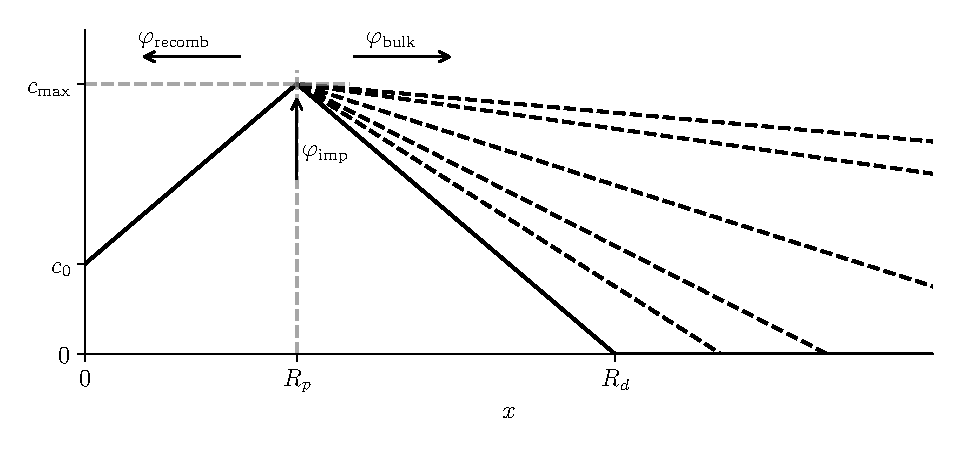
\includegraphics[width=0.75\linewidth]{Figures/Chapter2/recomb_sketch.pdf}
    \caption{Concentration profile with recombination flux and volumetric source term at $x=R_p$. Dashed lines correspond to time evolution.}
    \label{fig:recomb sketch}
\end{figure*}

The concentration profile is therefore maximum at $x=R_p$.
The expression of $c_\mathrm{max}$ can be obtained by expressing the flux balance at equilibrium:

\begin{equation}
    \varphi_\mathrm{imp} = -\varphi_\mathrm{recomb} + \varphi_\mathrm{bulk}
    \label{eq:flux balance}
\end{equation}
where $\varphi_\mathrm{recombination}$ is the recombination flux and $\varphi_\mathrm{bulk}$ is the migration flux.

$\varphi_\mathrm{bulk}$ can be expressed as:
\begin{equation}
    \varphi_\mathrm{bulk} = D \cdot \frac{c_\mathrm{max}}{R_d(t) - R_p}
\end{equation}

When $t \rightarrow \infty$ or $R_d \gg R_p$ (a ratio of 10 or 100 is enough), $\varphi_\mathrm{bulk} \ll \varphi_\mathrm{recomb}$.
According to Fick's law, Equation \ref{eq:flux balance} reads:

\begin{eqnarray}
    \varphi_\mathrm{imp} &= D \cdot \frac{c_\mathrm{max}-c_{0}}{R_{p}} \\
    \Leftrightarrow c_\mathrm{max} &= \frac{\varphi_\mathrm{imp} R_{p}}{D}+ c_0
    \label{eq:c_max}
\end{eqnarray}

Equation \ref{eq:flux balance} can also be written by expressing $\varphi_\mathrm{recombination}$ as a function of the recombination coefficient $K$:

\begin{eqnarray}
    \varphi_\mathrm{imp} &= K c_{0}^{2} \\
    \Leftrightarrow c_{0} &= \sqrt{\frac{\varphi_\mathrm{imp}}{K}}
    \label{eq:c_0}
\end{eqnarray}

By replacing Equation \ref{eq:c_0} in Equation \ref{eq:c_max} one can obtain:

\begin{equation}
    c_\mathrm{max} = \frac{\varphi_\mathrm{imp} R_{p}}{D}+\sqrt{\frac{\varphi_\mathrm{imp}}{K}}
\end{equation}

As the recombination process becomes fast (\textit{ie} $K \rightarrow \infty$), $c_0 \approx 0$ and $c_\mathrm{max} \approx \frac{\varphi_\mathrm{imp} R_{p}}{D}$.


\subsection{Interface conditions}
According to \sidecite{krom_hydrogen_2000} since the solubility of hydrogen atoms in solids is low, the chemical potential of solute hydrogen $\mu$ is expressed by:
\begin{equation}
    \mu = \mu_0 + RT \ln\left( \frac{c_\mathrm{m}}{N_L}\right)
\end{equation}
where $\mu_0$ is the chemical potential in a reference state in \si{J.mol^{-1}}, $R$ the ideal gas constant, $T$ the temperature in \si{K}, $c_\mathrm{m}$ the mobile hydrogen concentration in \si{m^{-3}} and $N_L$ the lattice site concentration in \si{m^{-3}}.

Assuming that only free hydrogen atoms contribute to the overall flux in the material, the particle flux $J$ in \si{m^{-2}.s^{-1}} can be expressed by Fick's law:
\begin{equation}
    J = - D \nabla c_\mathrm{m}
\end{equation}
where $D$ is the diffusion coefficient of hydrogen in a non-stress lattice expressed in \si{m^{2}.s^{-1}}. 


The local equilibrium at the interface between two materials must ensure  the continuity of both the chemical potential $\mu$ (see Equation \ref{eq: muconservation}) and the particle flux (see Equation \ref{eq: flux conservation}).
\begin{equation}
    \mu^- = \mu^+  \label{eq: muconservation}  
\end{equation}
    
\begin{equation}
    D^- \nabla c_\mathrm{m}^- = D^+ \nabla c_\mathrm{m}^+ \label{eq: flux conservation} 
\end{equation}
The chemical potential continuity can also be ensured by the continuity of the quantity $c_\mathrm{m}/S$ (see Equation \ref{eq: c/s conservation}) for mechanical stress-free materials in thermodynamic equilibrium and the Soret effect being neglected:
\begin{equation}
    \left(\frac{c_\mathrm{m}}{S}\right)^- = \left(\frac{c_\mathrm{m}}{S}\right)^+  \label{eq: c/s conservation}  
\end{equation}
Here, the quantity $c_\mathrm{m}/S$, with $S$ the solubility of hydrogen expressed in \si{m^{-3}.Pa^{-0.5}}, is equivalent to the root square of the pressure of an imaginary gas in thermodynamic equilibrium between the two solids and for which Sievert's law is applied.  

This assumption is correct as long as the time needed to reach the equilibrium is low compared to the time of the simulation.
For long exposure time as well as for high temperatures, it was shown in \sidecite{delaporte-mathurin_influence_2021} that the characteristic time is small enough for the equilibrium model to be valid.

From Equation \ref{eq: c/s conservation}, one can deduce that a solubility discontinuity across an interface induces a discontinuity of mobile hydrogen concentration $c_\mathrm{m}$.
This can also be interpreted as the chemical potentials at a reference state being different in different materials \sidecite{kirchheim_25_2014}, as the lattice site concentration.

To ensure a correct treatment of the material interface in hydrogen transport codes, two approaches can be employed.
The most straightforward approach is to solve the hydrogen mobile concentration transport in both materials (see Equation \ref{eq: diffusion equation}) and enforce the concentration jump at the interface between the two materials with an internal condition verifying  Equation \ref{eq: c/s conservation} \sidecite{longhurst_tmap7_2008}.

\begin{equation}
    \frac{\partial c_\mathrm{m}}{\partial t}=\nabla \cdot\left(D \nabla c_\mathrm{m}\right) + f
   \label{eq: diffusion equation}
\end{equation}
where $f$ is the source term in \si{m^{-3}.s^{-1}}.

Another method is to perform a change of variable in Fick's second law of diffusion with $\phi = c_\mathrm{m}/S$ \sidecite{smith_abaqusstandard_2009} when internal conditions cannot be set.
Equation \ref{eq: diffusion equation} therefore reads:

\begin{align}
    \frac{\partial \phi S}{\partial t} &= \nabla \cdot\left(D \nabla \phi S\right) + f \nonumber \\
    &=\nabla \cdot\left( D S \nabla \phi + D \phi \nabla S\right) + f \label{eq: diffusion equation changed}
\end{align}

Because $\phi$ is computed, the ratio $c_\mathrm{m}/S$ is continuous by default at the material interfaces.

This second approach is used for instance in the \textit{mass-diffusion} procedure of the Abaqus code \sidecite{smith_abaqusstandard_2009}.
This interface model has also been implemented into the current hydrogen transport code FESTIM \sidecite{delaporte-mathurin_finite_2019} using FEniCS \sidecite{alnaes_fenics_2015}.


\section{Heat transfer}
Due to the numerous processes that are thermally activated, it is essential have an accurate temperature field.
Moreover, most tokamak plasma facing components are exposed to intense heat fluxes and are actively cooled, exhibiting high temperature gradients.
The temperature fields are even more complex when dealing with non-trivial geometries like monoblocks or breeding blankets.
For these reasons, heat transfers need to be modelled.

\subsection{Bulk model}

The equation describing heat conduction in solids is described as follows:
\begin{equation}
    \rho \cdot C_p \frac{\partial T}{\partial t}=\nabla \cdot (\lambda \nabla T)
    \label{eq:heat equation}
\end{equation}
where $\rho$ is the density of the material in \si{kg.m^{-3}}, $C_p$ its specific heat capacity expressed in \si{J.kg^{-1}.K^{-1}} and $\lambda$ the thermal conductivity expressed in \si{W.m^{-1}.K^{-1}}.

The thermal properties $C_p$, $\rho$ and $\lambda$ are usually temperature dependent.

\subsection{Boundary conditions}

For heat transfer problems, three types of boundary conditions can be imposed.

First, the temperature can be fixed on the boundary (see Equation \ref{eq:dirichlet bc T}).
\begin{equation}
    T = T(x, y, z, t) \quad \text { on } \partial \Omega
    \label{eq:dirichlet bc T}
\end{equation}
where $\partial \Omega$ is the domain boundary.

On the other hand, a heat flux can also be imposed by enforcing the temperature gradient (see Equation \ref{eq: neumann bc T}).
\begin{equation}
    -\lambda \nabla T \cdot \mathbf{n} = f(x, y, z, t) \quad \text { on } \partial \Omega
    \label{eq: neumann bc T}
\end{equation}
where $\lambda$ is the thermal conductivity in \si{W.m^{-1}.K^{-1}}, $\mathbf{n}$ is the boundary normal vector and $\partial \Omega$ is the domain boundary.

Finally, to model a convective heat flux when the surface is in contact with a fluid (\textit{eg} cooling pipes, natural convection...), a Robin boundary condition needs to be employed (see Equation \ref{eq: convective bc T}).
\begin{equation}
    -\lambda \nabla T \cdot \mathbf{n} = h (T - T_\mathrm{ext}) \quad \text { on } \partial \Omega
    \label{eq: convective bc T}
\end{equation}
where $\lambda$ is the thermal conductivity in \si{W.m^{-1}.K^{-1}}, $\mathbf{n}$ is the boundary normal vector, $h$ is the heat exchange coefficient in \si{W.m^{-2}.K^{-1}}, $T_\mathrm{ext}$ is the fluid temperature in \si{K} and $\partial \Omega$ is the domain boundary.
The heat exchange coefficient is usually dependent on the temperature.

\section{Implementation}


The models described in this Section can be hard to solve analytically for complex problems (complex geometries, transients, combined boundary conditions, etc).
The code FESTIM \sidecite{delaporte-mathurin_finite_2019} was therefore developped in order to solve these equations numerically.

\subsection{The finite element method: FEniCS}
FESTIM is based on the Finite Element Method to solve this set of equations and boundary conditions.
Several finite element libraries are openly available (deal.II \sidecite{arndt_dealii_2021}, MFEM \sidecite{kolev_tzanio_modular_2010}, MOOSE \sidecite{permann_moose_2020}, FreeFEM++ \sidecite{hecht_new_2012}, ...).
The open-source python package FEniCS \sidecite{alnaes_fenics_2015} was employed.
The finite element method is a versatile tool that can solve any partial differential equation on an arbitrary geometry in 1D, 2D or 3D.
The main advantage of this method compared to the finite diference method is the simplicity of its application to complex geometries and unstructured meshes.
Indeed, implementing a finite difference scheme for such a problem would be tedious and extra care must be taken for mistakes in the implementation could result in losses in efficiency and accuracy of the numerical solution.

This section will detail the finite element method applied to a simple diffusion equation (see Equation \ref{eq: example poisson}).

\begin{equation}
    -\nabla^2 u = f
    \label{eq: example poisson}
\end{equation}

The first step of the finite element method is to represent the solution $u$ as a combination of polynomial expressions (see Equation \ref{eq: FEM solution}).

\begin{equation}
    u = \sum^N_{i=0}u_i \phi_i(x, y, z)
    \label{eq: FEM solution}
\end{equation}
where $u_i$ are the coefficient to be determined (called degrees of freedom) and $\phi_i$ are polynomials (see Figure \ref{fig: example approximated solution}).

\begin{marginfigure}
    \centering
    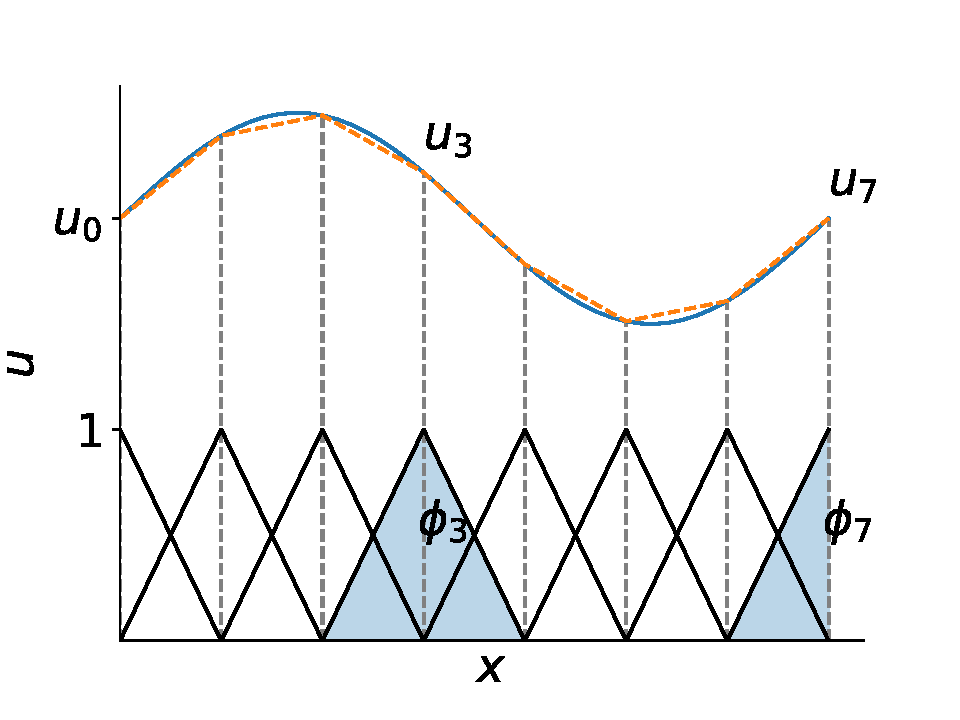
\includegraphics[width=\linewidth]{Figures/Chapter2/approximated_solution.pdf}
    \caption{Example of an approximated solution $u$ (exact in blue, approximated in orange) with basis functions $\phi_i$}
    \label{fig: example approximated solution}
\end{marginfigure}


The second step is to build a variational formulation (also called weak form) of the governing equation \ref{eq: example poisson}.
To do so, the recipe is to multiply the PDE by a function $v$ (called the test function) and integrate over an arbitrary element $\Omega_e$.
The following expression is obtained:
\begin{equation}
    \int_{\Omega_e} -\nabla^2 u v dx = \int_{\Omega_e} f v dx
    \label{eq: weak form 1}
\end{equation}

When using $N+1$ different test functions, Equation \ref{eq: weak form 1} then gives rise to a system of $N+1$ equations.
This form is called the weak form because it relaxes the requirement of Equation \ref{eq: example poisson} and instead requires to solve Equation \ref{eq: weak form 1} for all test functions.

Equation \ref{eq: weak form 1} needs now to be rewritten in order to only have first order derivatives.
To do so, Gauss-Green's lemma is employed:
\begin{equation}
    \int_{\Omega_e} -\nabla^2 u v dx = \int_{\Omega_e} \nabla u \cdot \nabla v dx - \int_{\partial \Omega_e} \frac{\partial u}{\partial n} v dx
    \label{eq: gauss-green}
\end{equation}

The variational form therefore reads:
\begin{equation}
    \int_{\Omega_e} \nabla u \cdot \nabla v dx = \int_{\Omega_e} f v dx + \int_{\partial \Omega_e} \frac{\partial u}{\partial n} v dx
    \label{eq: weak form 2}
\end{equation}
where the last term of the equation either vanishes due to Dirichlet boundary conditions or is imposed.

From Equation \ref{eq: weak form 2}, a system of $N+1$ equations can be solved that can be solved to determine the coefficients $c_i$ in Equation \ref{eq: FEM solution}
Once the $c_i$ coefficients are known, an approximated solution can be computed.

\subsection{Main features of FESTIM}
FESTIM provides an even higher level of abstraction than FEniCS by providing a user-friendly interface dedicated to H transport and H transfer problems.
Users only have to provide inputs such as material properties, traps properties, geometry, solving parameters, without having to dive into the finite element implementation.

% user friendly
Multi-dimensional transient simulations coupled with heat transfer can therefore be run fairly easily without finite element knowledge.
Nevertheless, since FESTIM is object-oriented, advanced users will always be able to turn FESTIM inside-out to adapt the code to their specific needs (specific boundary conditions, slight changes in the governing equations...).
Since FESTIM is written in python - which is a fairly easy-to-learn programming langage - no advanced level of coding is required.
For example, the simple code below is all that is required to simulate a bi-material case (see Figure \ref{fig: example FESTIM}).


\begin{lstlisting}[language=Python]

import FESTIM
import numpy as np

parameters = {
    "materials": [
        {  # material 1
            "D_0": 1,  # diffusion coefficient
            "E_D": 0.2,
            "borders": [0, 5],
            "id": 1
        },
        {  # material 2
            "D_0": 0.5,
            "E_D": 0.2,
            "borders": [5, 10],
            "id": 2
        },
    ],
    "boundary_conditions": [
        {
            "type": "dc",
            "value": 0,  # c_m = 0 on boundaries
            "surfaces": [1, 2],  # left and right
        }
    ],
    "source_term": {
        "value": 0.1  # volumetric source of H
    },
    "temperature": {
        "type": "expression",
        "value": 600 + 10*FESTIM.x
    },
    "traps": [
        {
            "k_0": 1,  # trapping rate
            "E_k": 0,
            "p_0": 1,  # detrapping rate
            "E_p": 0,
            "density": 10,
            "materials": [1]
        }
    ],
    "mesh_parameters": {
        "vertices": np.linspace(0, 10, num=500)
    },
    "exports": {},
    "solving_parameters": {
        "type": "solve_stationary",
        "newton_solver": {
            "absolute_tolerance": 1e-10,
            "relative_tolerance": 1e-10,
            "maximum_iterations": 15
        },
        "traps_element_type": "DG"
    }
}

output = FESTIM.run(parameters)

from fenics import plot
import matplotlib.pyplot as plt

plot(output["solutions"]["retention"])
plt.show()
\end{lstlisting}

\begin{marginfigure}
    \centering
    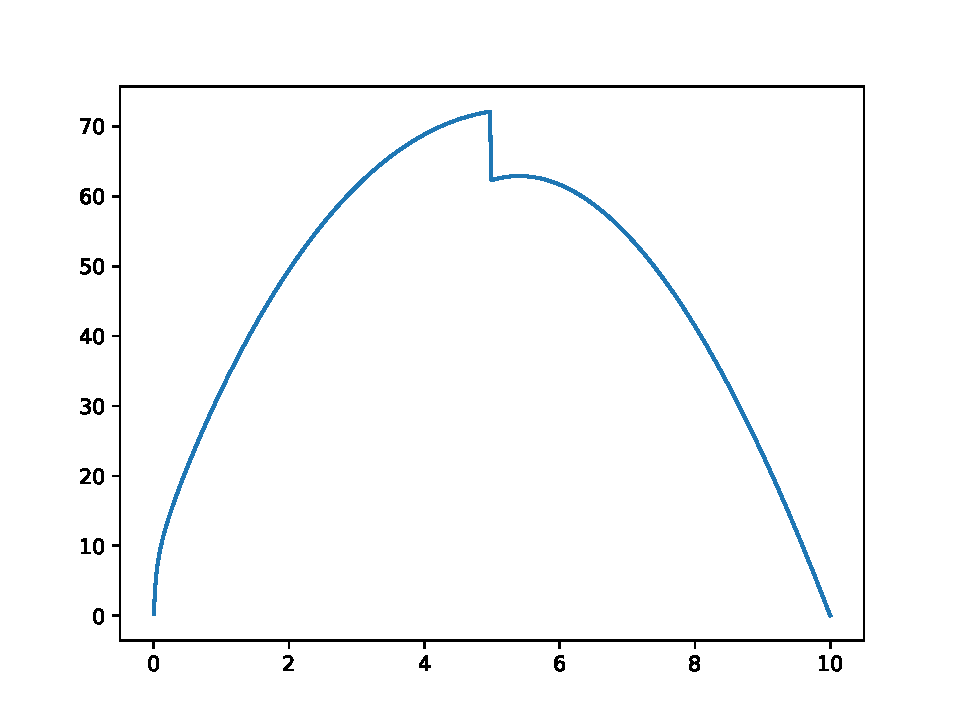
\includegraphics[width=\linewidth]{Figures/Chapter2/example.pdf}
    \caption{Example retention profile in a bi-material case produced by FESTIM}
    \label{fig: example FESTIM}
\end{marginfigure}

% physics
As mentioned above, FESTIM simulates the transport (diffusion and trapping) of H and additional physics can be incorporated, such as the Soret effect (also called heat of transport) and conservation of chemical potential at interfaces...
Various types of boundary conditions are available for both the H transport (imposed concentration, recombination flux, dissociation flux, implanted source approximation...) and the heat transfer problems (imposed temperature, imposed flux, convective flux...).
Traps densities in FESTIM can also be time-dependent allowing the users to simulate extrinsic traps (\textit{eg} irradiation induced traps, stress induced traps...).

% geometry
Thanks to the finite element method, geometries used in FESTIM can be complex (see Figure \ref{fig: example mesh}).
The meshing capability of FESTIM is limited to 1D meshes and it was decided to instead make FESTIM accept (with the XDMF format) complex meshes from third-party applications dedicated to meshing such as SALOME or GMSH.
These third-party applications can for instance be usefull to run CAD-based simulations.
Users can also decide to use the FEniCS built-in meshing tool.

\begin{marginfigure}
    \centering
    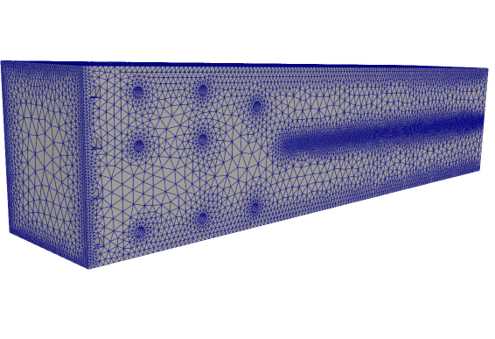
\includegraphics[width=\linewidth]{Figures/Chapter2/example_mesh.png}
    \caption{Example of a complex 3D breeding blanket mesh readable by FESTIM}
    \label{fig: example mesh}
\end{marginfigure}

% visualisation
Similarly, FESTIM (FEniCS) visualisation functions are limited.
FESTIM is not a graphical application but the files generated by FESTIM (XDMF, CSV, TXT) can easily be read and post-processed by specialised tools such as Paraview \sidecite{ahrens_paraview_2005}, matplotlib \sidecite{hunter_matplotlib_2007}, NumPy \sidecite{harris_array_2020}, etc.

% what FE
Regarding the default finite elements used in FESTIM are Continuous Galerkin elements but it can be switched to Discontinuous Galerkin when needed.
This is usefull when the trapped concentration is discontinuous and help avoiding under- or over-shoots in the concentration field.

% Adaptive step size
When dealing with transient problems, FESTIM provides an adaptive stepsize allowing the stepsize to increase (by a user-defined factor) when the convergence criterion is easily reached.
This greatly improve the performance of the code since less timesteps need to be computed.



\section{Verification \& Validation}
\subsection{Analytical verification}
Verification is the process of ensuring the governing equations are correctly solved in FESTIM.
This is an integral part of every simulation code for it guarantees the code is error free.
It is generally hard to simply substitute this process by code comparison (cross-checks between two different codes) because often the codes are implemented differently.
Moreover, if the code we are comparing with is not verified, then obtaining similar results does not give any guarantee on the code accuracy.

Several methods can be used to verify a code but the Method of Exact Solutions (MES) and the Method of Manufactured Solutions (MMS) are employed here.

Both methods consist in comparing a computed solution with an exact solution and measuring the error.
The exact solution in the MES is obtained by solving the governing equations analytically.
When using the MMS, on the other hand, the problem is reversed: an arbitrary exact solution (called \textit{manufactured solution}) is chosen and injected in the governing equations.
It is then possible to determine source terms and boundary conditions.
These are then fed into the code and the computed solution is compared to the manufactured (exact) solution.

This MMS method is often used to unravel the complexity of governing equations \sidecite{dudson_verification_2016, roache_code_2002}.
This is particularly usefull when dealing with complex geometries or to exercise non-trivial material propoerties.

\subsubsection{H transport (MES)} \label{analytical}

% Although validation against experiments could show that FESTIM is able reproduce the data with a given set of parameters, objective verification against analytical solutions is first required to ensure that the governing Equations \ref{eq:mobile} and \ref{eq:trapped} are solved correctly.

For this verification case, a 1D slab is considered with a thickness $l$.
The concentration of mobile particles was set to $c_0$ on one side of the slab and set to zero on the other side.
Only one trap is considered in this case and its density $n_1$ is homogeneously distributed.

The trapping parameter $\zeta$ is defined in \sidecite{longhurst_verification_2005} as follow:
\begin{equation}
    \zeta = \frac{\lambda^2 \: n_\mathrm{solute} \: \nu_0}{D_0 \: n_1}\exp\bigg(\frac{E_\mathrm{diff} - E_1}{k_B \: T}\bigg) + \frac{c_\mathrm{m}}{n_1}
\end{equation}

In our case, we choose the detrapping energy $E_1$, the concentration $c_0$ and the temperature $T$ so that $\zeta \gg \frac{c_\mathrm{m}}{n_1}$.
This is known as the \textit{effective diffusivity regime} where the diffusion is almost identical to the case where there are no traps.
The coefficient $D$ is then replaced by an effective diffusion coefficient:
\begin{equation}
    D_\mathrm{eff} = \frac{D}{1+\frac{1}{\zeta}}
\end{equation}
The particle flux at the background surface is expressed in $\SI{}{H.m^{-2}.s^{-1}}$ and finally defined in \sidecite{longhurst_verification_2005} by:
\begin{equation}
    \varphi_H(t) = \frac{c_0 D}{l}\bigg[1+2\sum_{m=1}^{\infty}(-1)^m \exp\bigg(-m^2\frac{\pi^2 \:D_\mathrm{eff} \: t}{l^2}\bigg)\bigg]
\label{eq:flux analytical}
\end{equation}
All the parameters are defined in Table \ref{tab:parameters analytical verification}.
These parameters have been chosen for the sake of verification and do not necessarily represent realistic conditions as verification is a mathematical exercise.
\begin{table}
    \centering
    \begin{tabular}{p{2.3cm} p{2cm} r}
        Parameter & Units & Value \\
        \hline
        \\
        $\rho$ & $\si{m^{-3}}$ &$\SI{3.16e22}{}$ \\
        $n_1$ & & $\SI{1.00e-1}{} \rho$ \\
        $c_0$ & & $\SI{1.00e-4}{} \rho$\\
        $n_\mathrm{solute}$ & & $2 \:\rho$\\
        \\
        $E_1$ & $\si{eV}$ & $\SI{8.6e-3}{}$ \\
        $E_\mathrm{diff}$ & & $0$ \\
        \\
        $\lambda$ & $\si{m}$ & $\SI{3.16e-8}{}$  \\
        $l$ & & $\SI{5e-5}{}$\\
        \\
        $T$ & $\si{K}$ & 1000 \\
        \\
        $t_f$ & $\si{s}$ & \SI{e-8}{} \\
        $\nu_0$ & $\si{s^{-1}}$ & $\SI{e13}{}$ \\
        $D_0$ & $\si{m^2.s^{-1}}$ & $1$ \\
        \\
    \end{tabular}
    \caption{Parameters used for the analytical verification}
    \label{tab:parameters analytical verification}
\end{table}
One can notice on Figure \ref{fig:FESTIM vs analytical} that the numerical results are in good agreement with the analytical solution.
The maximum error between analytical and numerical solutions is calculated to be \SI{6.56e20}{H.m^{-2}.s^{-1}} with 50000 piecewise linear elements (P1) which corresponds to \SI{1}{\%} of the maximum value.
According to finite elements theory, this value will decrease with the stepsize and with the element size.
\begin{figure}
    \centering
    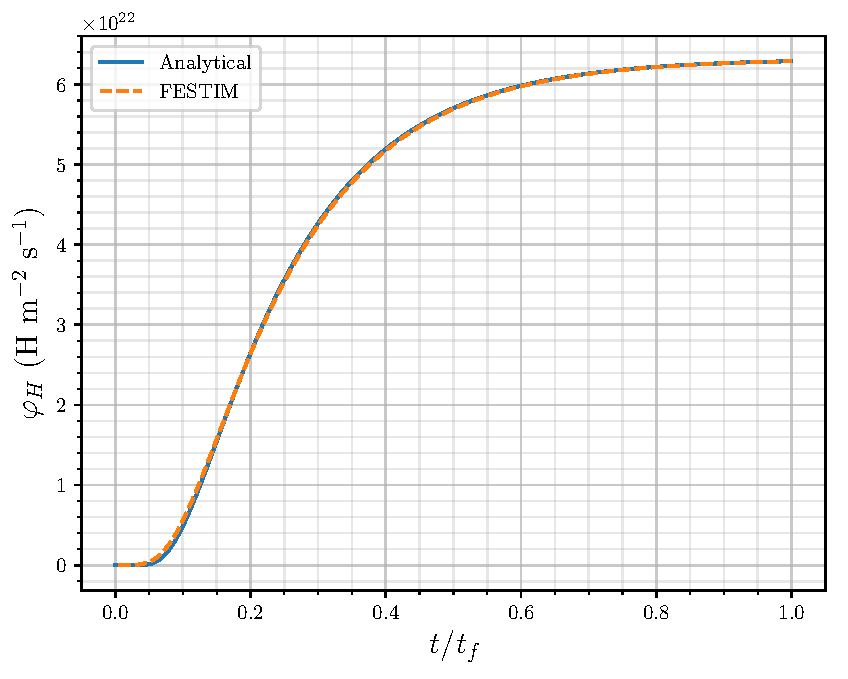
\includegraphics[width=\linewidth]{Figures/Chapter3/FESTIM_vs_analytical.pdf}
    \caption{Temporal evolution of the particle flux $\varphi_H$ ($t_f = \SI{e-8}{s}$)}
    \label{fig:FESTIM vs analytical}
\end{figure}

Since this test case is very similar to a pure diffusion case, it does not exercise all terms of the governing equations.
To do so, the governing equations would have to be solved for a generic case which proves to be complex.
This is why the MMS will be used instead.

\subsubsection{H transport (MMS)} \label{mms}

In order to exercise all terms of Equations \ref{eq:mobile} and \ref{eq:trapped}, the following manufactured solutions are chosen:
\begin{equation}
    \begin{cases}
    c_{m_D} = 1 + x^2 + \sin(t) \\
    c_{{t,1}_D} = 1 + x^2 + \cos(t)
    \end{cases}
    \label{eq: manufactured solutions}
\end{equation}

By combining Equations \ref{eq:mobile}, \ref{eq:trapped} and \ref{eq: manufactured solutions}, one can obtain the following source terms:
\begin{equation}
    \begin{cases}
    f = \cos(t) - \sin(t) - 2D \\
    g_1 = \nu_1 c_{{t,1}_D} - \nu_m c_{m_D} ( n_1 - c_{{t,1}_D}) - \sin(t)
    \end{cases}
    \label{eq:sources}
\end{equation}

where $g_1$ is an additional source term in Equation \ref{eq:trapped}.
The Dirichlet boundary conditions for $c_\mathrm{m}$ and $c_{t,1}$ are:

\begin{equation}
    \begin{cases}
    c_\mathrm{m} = 1 + x^2 + \sin(t) \quad \text{on } \partial \Omega \\
    c_{t,1} = 1 + x^2 + \cos(t) \quad \text{on } \partial \Omega 
    \end{cases}
\end{equation}
where $\partial\Omega$ is the boundary of the domain.
Finally, initial values for $c_\mathrm{m}$ and $c_{t,i}$ are:
\begin{equation}
    \begin{cases}
    c_\mathrm{m}(t=0) = 1 + x^2 \\
    c_{t,1}(t=0) = 2 + x^2
    \end{cases}
\end{equation}
Once all these parameters are fed into FESTIM, one can easily compare the computed solution with the exact solution in Equation \ref{eq: manufactured solutions}.
The L2-norm $E_{c_\mathrm{m}}$ can then be calculated as follow:
\begin{equation}
    E_{c_\mathrm{m}} = \sqrt{\int_\Omega(c_{m_D} - c_\mathrm{m})^2dx}
\end{equation}
The evolution of $E_{c_\mathrm{m}}$ as function of the element size $h$ is shown on Figure \ref{fig:error vs h}.
One can notice that $E_{c_\mathrm{m}}$ increases as $A\cdot h^k$.
This is known as the \textit{asymptotic regime} and the coefficient $k$ is called the convergence rate.
$k$ typically tends to N+1 as $h$ approaches $0$, $N$ being the order of the finite elements.
In this simulation, $k$ approaches $2$ as expected since elements of order $1$ have been used.

\begin{figure}
    \centering
    \includegraphics[width=1\linewidth]{"Figures/Chapter3/L2 error on Cm vs h"}
    \caption{Evolution of the L2 norm of the error as function of element size h}
    \label{fig:error vs h}
\end{figure}

The same method can be applied to a 2D case.
Let us choose the following steady state test problem on a domain $\Omega = [0, 1] \times [0, 1]$ with the manufactured solution $c_D(x, y) = \sin(\omega \pi x) \sin(\omega \pi y)$.

\begin{align}
    \nabla \cdot D \nabla c_\mathrm{m} &= -f_1 \\
    k c_\mathrm{m} (n - c_\mathrm{t}) - p c_\mathrm{t} &= -f_2 \\
    c_\mathrm{m} &= c_\mathrm{t} = c_D \text{  on  } \partial \Omega \\
    D &= 2 \\
    p &= 3 \\
    k &= 2 \\
\end{align}

The source terms $f_1$ and $f_2$ and the boundary conditions can be obtained in a similar fashion by replacing $c_\mathrm{m}$ and $c_\mathrm{t}$ in the governing equations.

It was shown that the computed solutions was similar to the exact solutions (see Figure \ref{fig: results MMS 2D H transport}).
Moreover, the convergence rates confirm the mesh dependency of the computed solutions accuracy (see Figure \ref{fig: convergence rates H}).
A super-convergence is observed for the P2 elements.

\begin{figure*}
    \centering
    \begin{subfigure}{0.3\linewidth}
        \centering
        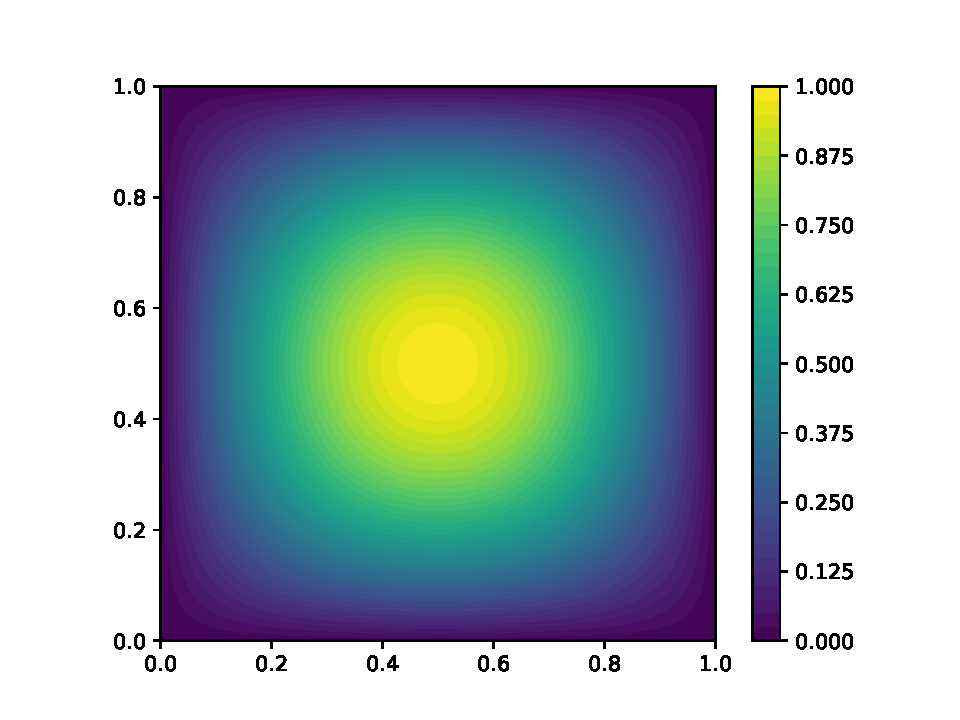
\includegraphics[width=\linewidth]{Figures/Chapter2/c_m.pdf}
        \caption{Computed $c_\mathrm{m}$ $N=64$}
    \end{subfigure}%
    \begin{subfigure}{0.3\linewidth}
        \centering
        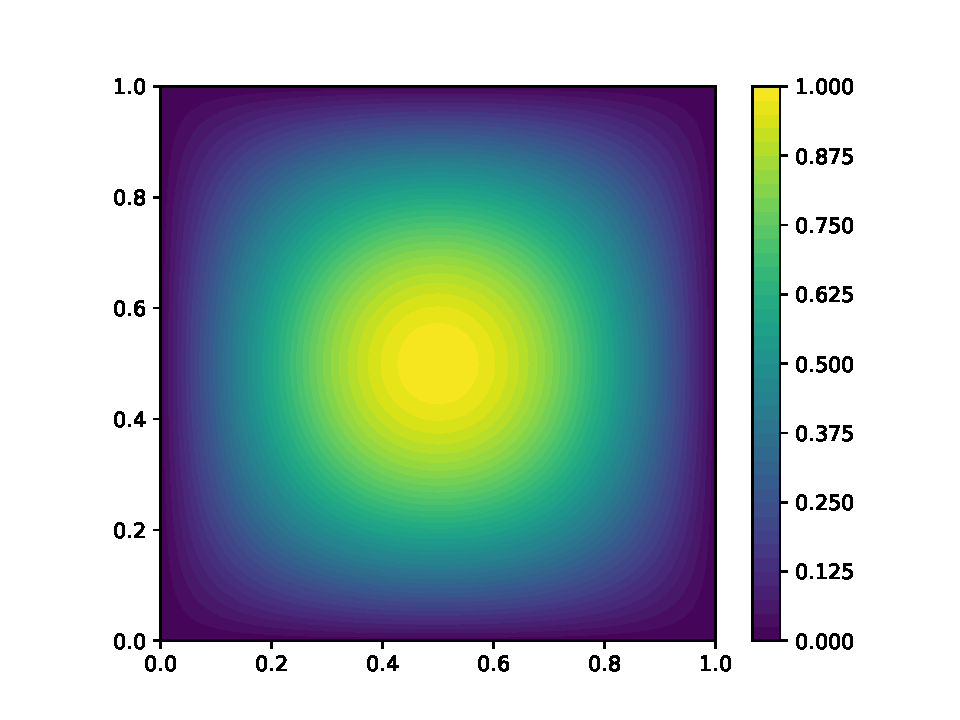
\includegraphics[width=\linewidth]{Figures/Chapter2/c_t.pdf}
        \caption{Computed $c_\mathrm{t}$ $N=64$}
    \end{subfigure}%
    \begin{subfigure}{0.3\linewidth}
        \centering
        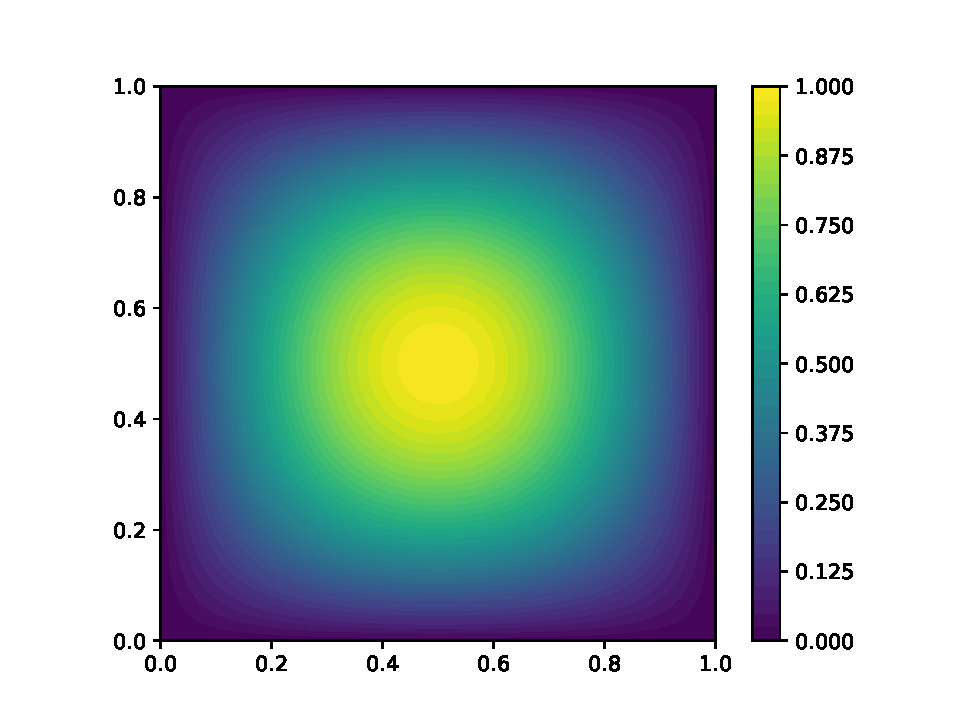
\includegraphics[width=\linewidth]{Figures/Chapter2/c_exact.pdf}
        \caption{Exact solution $c_D$}
    \end{subfigure}
    \caption{Comparison of the computed concentrations with the exact solution}
    \label{fig: results MMS 2D H transport}
\end{figure*}

\begin{figure}
    \centering
    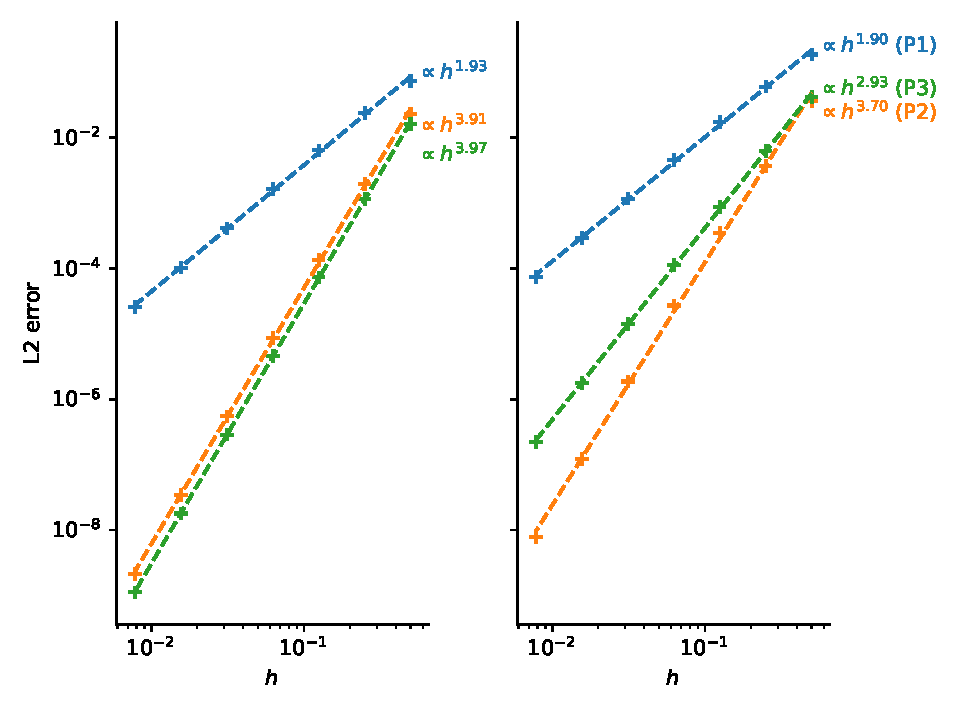
\includegraphics[width=\linewidth]{Figures/Chapter2/convergence_rate_H.pdf}
    \caption{Convergence rates}
    \label{fig: convergence rates H}
\end{figure}

\subsubsection{Conservation of chemical potential (MES)}
This verification case aims at checking the FESTIM code is correctly solving the governing Equations \ref{eq: flux conservation}, \ref{eq: c/s conservation}, \ref{eq: diffusion equation} and \ref{eq: diffusion equation changed}.

\begin{figure*} [h]
    \centering
    \begin{subfigure}{0.5\linewidth}
        \centering
        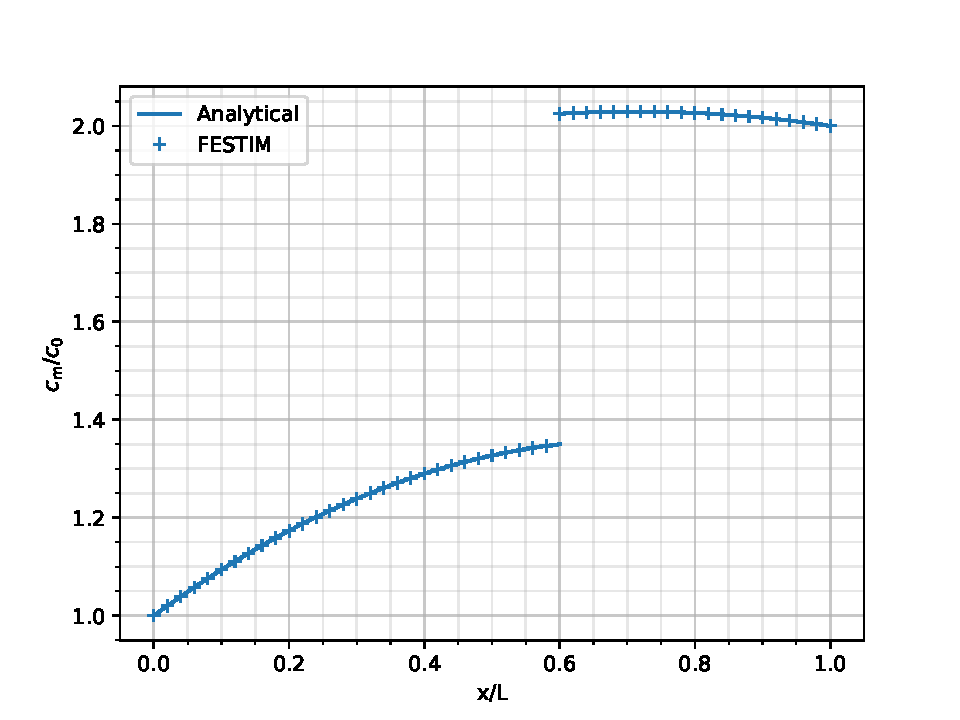
\includegraphics[width=\linewidth]{Figures/Chapter3/monoblocks/interface_condition/out_MES_case1.pdf}
        \caption{Case 1: $\alpha = 2$, $\beta = 1.5$, $\gamma=0.6$, $\tilde{c}_L = 2$, $\tilde{f}=1$}
    \end{subfigure}%
    % \hfill
    \begin{subfigure}{0.5\linewidth}
        \centering
        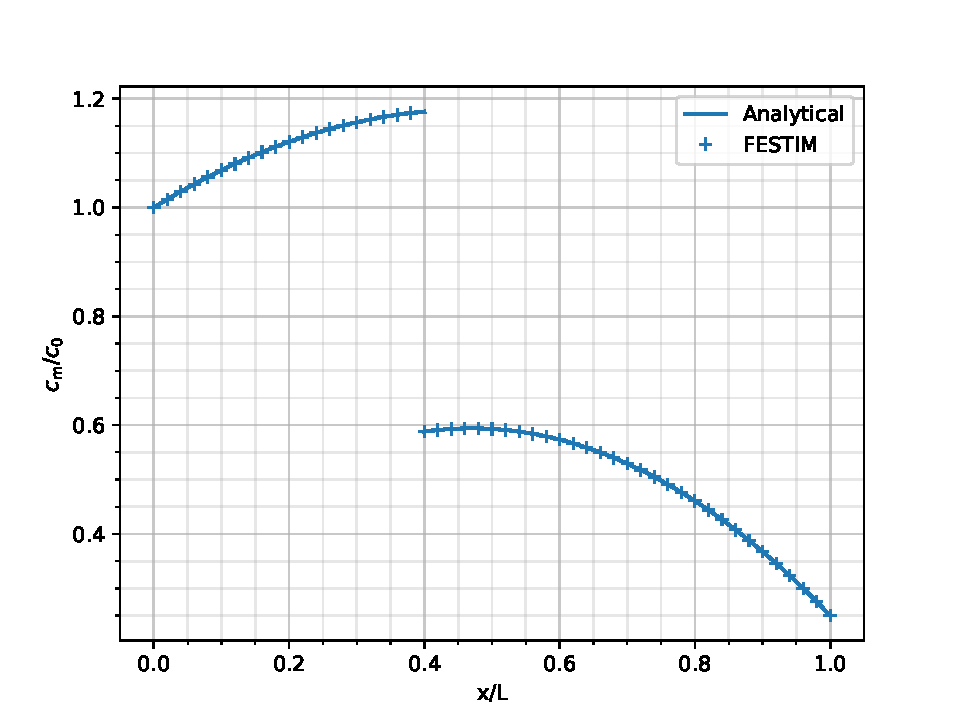
\includegraphics[width=\linewidth]{Figures/Chapter3/monoblocks/interface_condition/out_MES_case2.pdf}
        \caption{Case 2:  $\alpha = 1.5$, $\beta = 0.5$, $\gamma=0.4$, $\tilde{c}_L = 0.25$, $\tilde{f}=2$}
    \end{subfigure}
    \caption{Concentration profiles simulated by FESTIM against analytical solutions.}
    \label{fig:comparison MES}
\end{figure*}

The uni-dimensional test case considered in this Section was made of two subdomains $\Omega_1$ and $\Omega_2$ and is described as follow:
\begin{subequations}
\begin{align}
    \Omega &= [0, L] = \Omega_1 \cup \Omega_2 \\
    \Omega_1 &= [0, x_\mathrm{int}] \\
    \Omega_2 &= [x_\mathrm{int}, L] \\
    D &= \begin{cases}
        D_1,& \text{ in } \Omega_1\\
        D_2,& \text{ in } \Omega_2
    \end{cases} \\
    S &= \begin{cases}
        S_1,& \text{ in } \Omega_1\\
        S_2,& \text{ in } \Omega_2
    \end{cases}
\end{align}
\end{subequations}

The following dimensionless quantities are introduced:
\begin{subequations}
    \begin{align}
        \tilde{c}_\mathrm{m} &= c_\mathrm{m} / c_0\\
        \tilde{x} &= x / L \\
        \tilde{f} &= f \frac{L^2}{D_\mathrm{eq} c_0} \\
        \alpha &= D_2/D_1 \\
        \beta &= S_2/S_1 \\
        \gamma &= x_\mathrm{int}/L\\
    \end{align} 
\end{subequations}
where $D_\mathrm{eq} = (D_1 D_2)^{1/2}$.

By integrating Equation \ref{eq: diffusion equation} and assuming steady-state (\textit{i.e.} $\partial c/\partial t=0$), one can obtain the following dimensionless form:

\begin{equation}
        \tilde{c}_\mathrm{m}= 
\begin{cases}
    -\frac{1}{2}\alpha^{1/2}\tilde{f} \tilde{x}^2 + a_1 \tilde{x} + b_1,& \text{ in } \Omega_1\\
    -\frac{1}{2}\alpha^{-1/2}\tilde{f} \tilde{x}^2 + a_2 \tilde{x} + b_2,& \text{ in } \Omega_2
\end{cases}
\label{eq:MES c}
\end{equation}

where $a_1$, $b_1$, $a_2$, $b_2$ are the unknowns of the problem to be determined.
The boundary conditions and the equilibrium law at the interface are defined as:
\begin{subequations} \label{eq: bcs MES}
\begin{align} 
        \tilde{c}_\mathrm{m}(\tilde{x}=0) & = 1 \\
        \tilde{c}_\mathrm{m}(\tilde{x}=1) & =  \tilde{c}_L \\
        \tilde{c}_\mathrm{m}^-(\tilde{x}=\gamma) & =  \beta \; \tilde{c}_\mathrm{m}^+(\tilde{x}=\gamma)\\
        \nabla \tilde{c}_\mathrm{m}^-(\tilde{x}=\gamma) & =  \alpha \nabla \tilde{c}_\mathrm{m}^+(\tilde{x}=\gamma)
\end{align}
\end{subequations}


Equation \ref{eq:MES c} can be solved with these constraints and coefficients describing $\tilde{c_\mathrm{m}}$ therefore read:

\begin{align}
    \begin{split}
        a_1 &= a_0 \; \alpha^{1/2}  \\
        b_1 &= 1 \\
        a_2 &= a_0 \; \alpha^{-1/2}\\
        b_2 &= \tilde{c}_L + \frac{1}{2} \alpha^{-1/2} \tilde{f} - a_2 \\
        a_0 &= \frac{2 \alpha^{1/2}( \tilde{c}_L - \beta) + \tilde{f} \gamma^{2} ( 1 - \alpha \beta)}{2 \left( 1  - \gamma + \alpha \beta \gamma \right)} \\
    \end{split}
    \label{eq: MES c coefficients}
\end{align}

It is worth noting that when $\beta=1$ (\textit{i.e.} $S_1 = S_2 = S$) the solution becomes independent of $S$ and {$c_\mathrm{m}^{-}(x_\mathrm{int}) = c_\mathrm{m}^{+}(x_\mathrm{int})$}.
Moreover, when $\alpha = 1$ (\textit{i.e.} $D_1 = D_2 = D$), then $a_1 = a_2 = a_0$ which is the solution for steady-state diffusion in a mono-material.

The solution computed by FESTIM was found to be in very good agreement with the analytical solution for several test cases (see Figure \ref{fig:comparison MES}).

 
However, this method does not exercise all the terms in the governing Equation \ref{eq: diffusion equation changed}.
For instance, this analytical solution is only uni-dimensional, steady state is assumed and material properties are constant within the materials.
Having an exact solution from an analytical resolution for a general problem (multidimensional, transient, heterogeneous material properties, etc...) is often complex.
In order to exercise all these terms, the Method of Manufactured Solutions (MMS) will therefore be employed for it offers a good alternative to unravel these complexities.

\subsubsection{Conservation of chemical potential (MMS)}

This verification case aims at checking the FESTIM code is correctly solving the governing Equations \ref{eq: flux conservation}, \ref{eq: c/s conservation}, \ref{eq: diffusion equation} and \ref{eq: diffusion equation changed}.

The domain $\Omega$ for this test problem is a unit square composed of two subdomains $\Omega_1$ and $\Omega_2$ (see Equation \ref{eq: MMS domain}).
\begin{subequations} \label{eq: MMS domain}
\begin{align}
    \Omega &= [0, 1] \times [0, 1] \\
    \Omega_1 &= [0, x_\mathrm{int}] \times [0, 1] \\
    \Omega_2 &= [x_\mathrm{int}, 1] \times [0, 1] \\
\end{align}
\end{subequations}
In order to unravel the complexity of an analytical resolution of the direct problem, a manufactured solution $c_\mathrm{m}$ was constructed (see Equation \ref{eq: manufactured solution}) and the problem was solved backwards.

\begin{equation}
        c_M= 
\begin{cases}
    c_{M1},& \text{ on } \Omega_1\\
    \frac{S_2}{S_1} \cdot c_{M1},& \text{ on } \Omega_2
\end{cases}
\label{eq: manufactured solution}
\end{equation}
where $c_{M1} = 2 + \cos(2\pi x) \cdot \cos(2\pi y) + t$

It is worth noting that, when choosing a manufactured solution, one must ensure it satisfies all the governing equations (especially Equations \ref{eq: flux conservation} and \ref{eq: c/s conservation}).
In our case, $c_M$ ensures the flux conservation at the interface and the continuity of the quantity $c_\mathrm{m}/S$.

Properties are assumed time and space dependent in order to test every portion of the code (see Equation \ref{eq: MMS properties}).
\begin{subequations}
    \begin{align}
        D_1(x, y, t) & =  D_{1_0} \exp(-E_{D_1}/(k_B \cdot T(x,y, t) )) \\
        D_2(x, y, t) & =  D_{2_0} \exp(-E_{D_2}/(k_B \cdot T(x,y, t) )) \\
        S_1(x, y, t) & =  S_{1_0} \exp(-E_{S_1}/(k_B \cdot T(x,y, t) )) \\
        S_2(x, y, t) & =  S_{2_0} \exp(-E_{S_2}/(k_B \cdot T(x,y, t) )) \\
        T(x, y, t) & = 500 + 30 \cos(2\pi x) \cos(2 \pi y) \cos(2 \pi t)
\end{align} \label{eq: MMS properties}
\end{subequations}
with ${k_B = \SI{8.617e-5}{eV.K^{-1}}}$ the Boltzmann constant, $D_{1_0} = 1$, $E_{D_1} = 0.1$, $D_{2_0} = 2$, $E_{D_2} = 0.2$, $S_{1_0} = 1$, $E_{S_1} = 0.1$, $S_{2_0} = 2$ and $E_{S_2} = 0.2$.
The temperature $T$ varies around \SI{500}{K} so that, given the activation energies, properties do not approach zero.

By injecting the manufactured solution $c_M$ into the governing Equation \ref{eq: diffusion equation}, the source term can be expressed as:
\begin{align}
    f(x, y, t) &= \frac{\partial c_M}{\partial t} - \vec{\nabla} \cdot\left(D(x, y)
    \vec{\nabla}c_M\right) \nonumber \\
    &= \begin{cases}
        \frac{\partial c_{M_1}}{\partial t} - \vec{\nabla} \cdot\left(D_1(x, y)
    \vec{\nabla}c_{M_1}\right),& \text{ on } \Omega_1\\
    \frac{\partial c_{M_2}}{\partial t} - \vec{\nabla} \cdot\left(D_2(x, y)
    \vec{\nabla}c_{M_2}\right),& \text{ on } \Omega_2\\
    \end{cases}
\end{align}

The source term $f$ was then fed into FESTIM alongside with the initial and boundary conditions described below:
\begin{subequations}
    \begin{align}
        c_\mathrm{m}(x, y, t) &= c_M(x, y, t), \text{ on } \partial \Omega \\
        c_\mathrm{m}(x, y, t=0) &= c_M(x, y, t=0), \text{ on } \Omega
    \end{align}
\end{subequations}

The computed solution $c_\mathrm{comp}$ can then be compared with the manufactured solution $c_M$ in order to quantitatively measure the numerical error.
After running the MMS process, the computed solution and the manufactured solution were in very good agreement at several arbitrarily chosen times of simulation (see Figure \ref{fig: results MMS}).
% The stepsize was $\Delta t=0.01$.
The absolute difference between the manufactured solution and the computed one was found to be zero on the boundary and maximum at the interface between the two materials.
This is explained by the Dirichlet boundary conditions enforcing the computed solution on the boundary.
This difference decreases by increasing the mesh refinement and decreasing the stepsize.
Nonetheless, the error was found to remain orders of magnitude lower than the actual solution.

\begin{figure*}
    \centering
    \begin{subfigure}{0.33\linewidth}
        \centering
        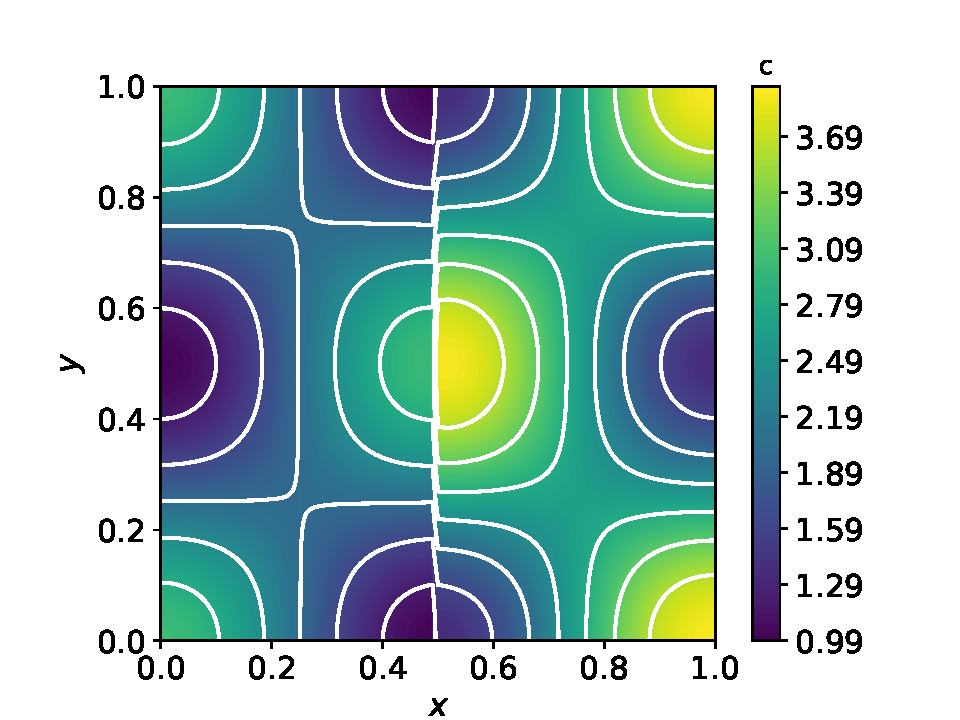
\includegraphics[width=\linewidth]{Figures/Chapter3/monoblocks/interface_condition/u_computed_t0.01.pdf}
        \caption{Computed solution $c_\mathrm{comp}(t=0.01)$}
    \end{subfigure}%
    \begin{subfigure}{0.33\linewidth}
        \centering
        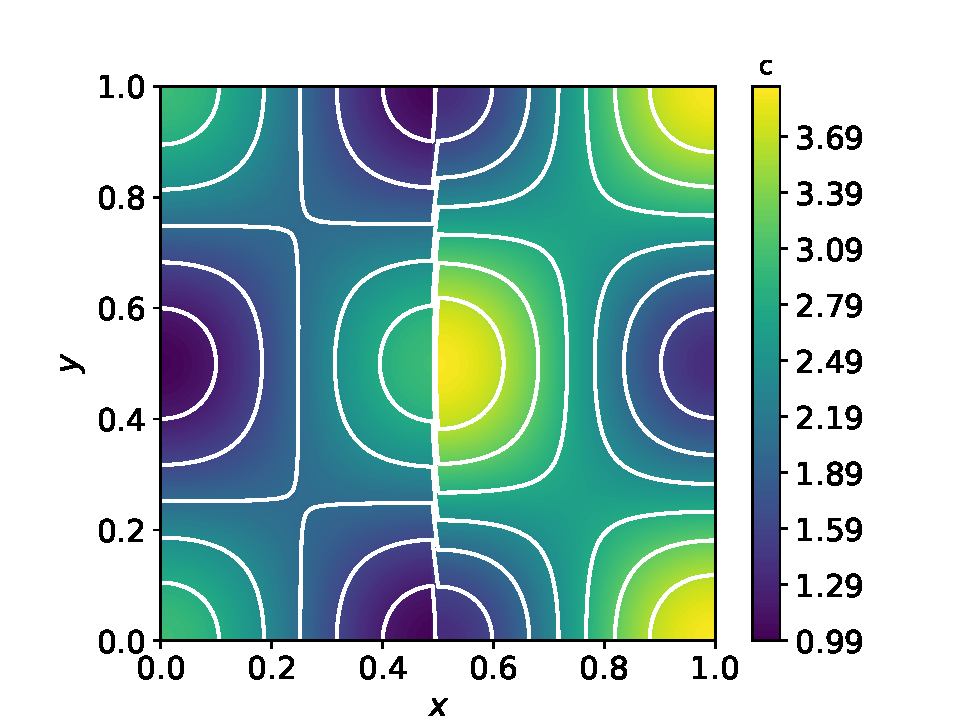
\includegraphics[width=\linewidth]{Figures/Chapter3/monoblocks/interface_condition/u_exact_t0.01.pdf}
        \caption{Exact solution $c_M(t=0.01)$}
    \end{subfigure}%
    \begin{subfigure}{0.33\linewidth}
        \centering
        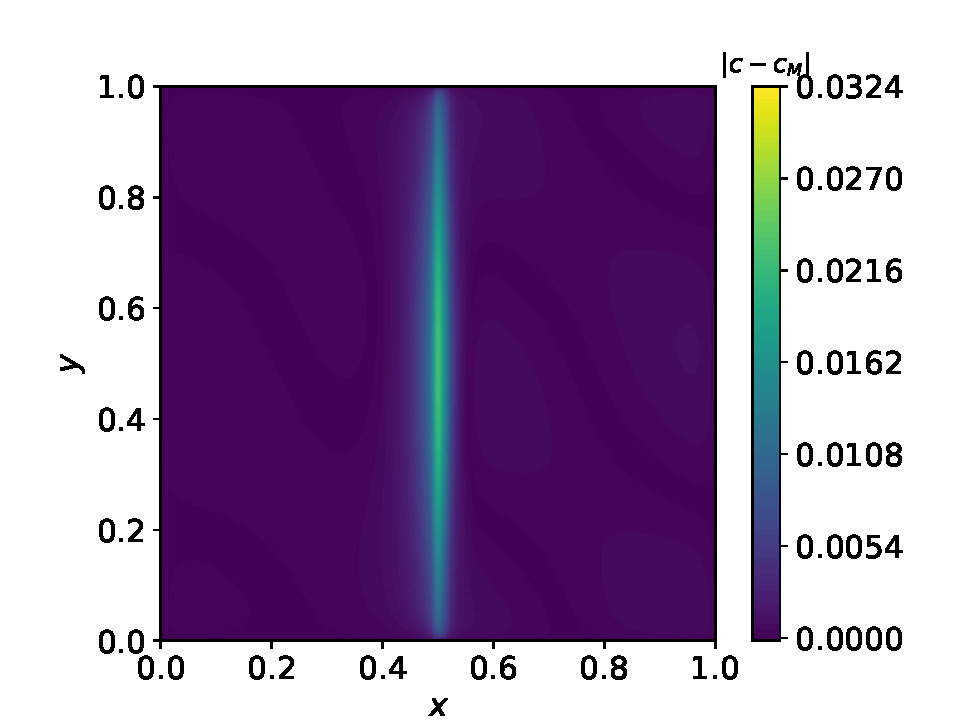
\includegraphics[width=\linewidth]{Figures/Chapter3/monoblocks/interface_condition/diff_t0.01.pdf}
        \caption{Absolute difference}
    \end{subfigure}
    \begin{subfigure}{0.33\linewidth}
        \centering
        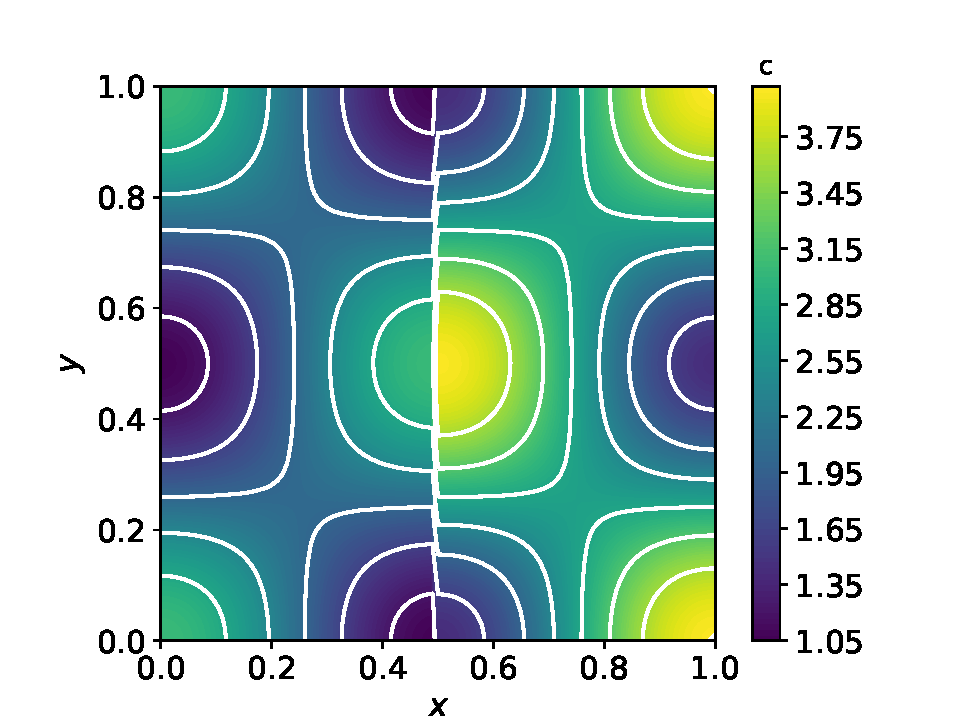
\includegraphics[width=\linewidth]{Figures/Chapter3/monoblocks/interface_condition/u_computed_t0.06.pdf}
        \caption{Computed solution $c_\mathrm{comp}(t=0.06)$}
    \end{subfigure}%
    \begin{subfigure}{0.33\linewidth}
        \centering
        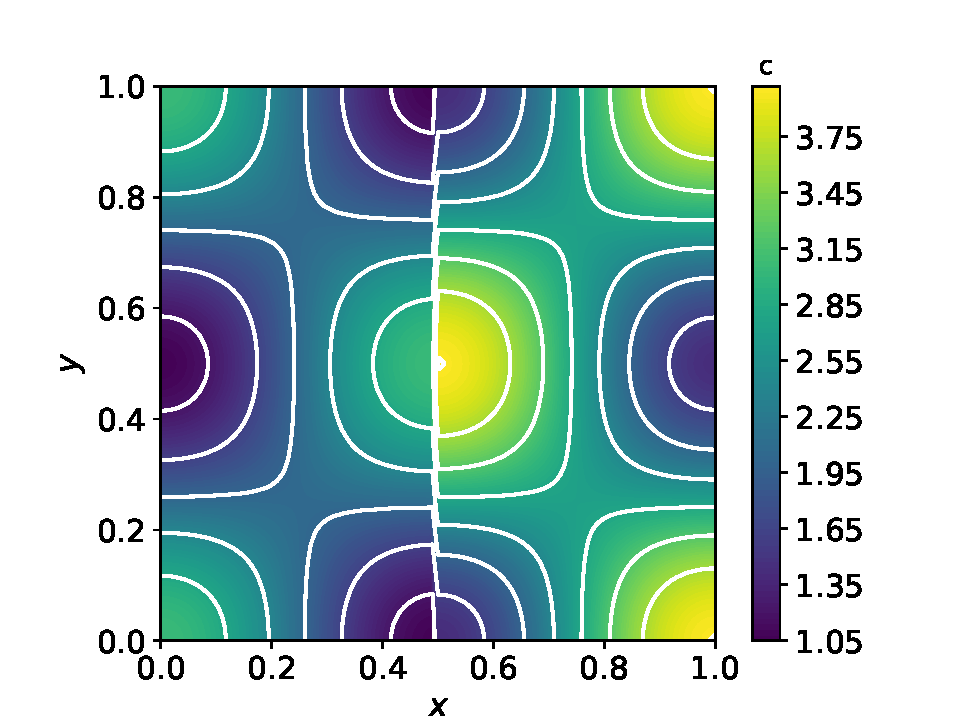
\includegraphics[width=\linewidth]{Figures/Chapter3/monoblocks/interface_condition/u_exact_t0.06.pdf}
        \caption{Exact solution $c_M(t=0.06)$}
    \end{subfigure}%
    \begin{subfigure}{0.33\linewidth}
        \centering
        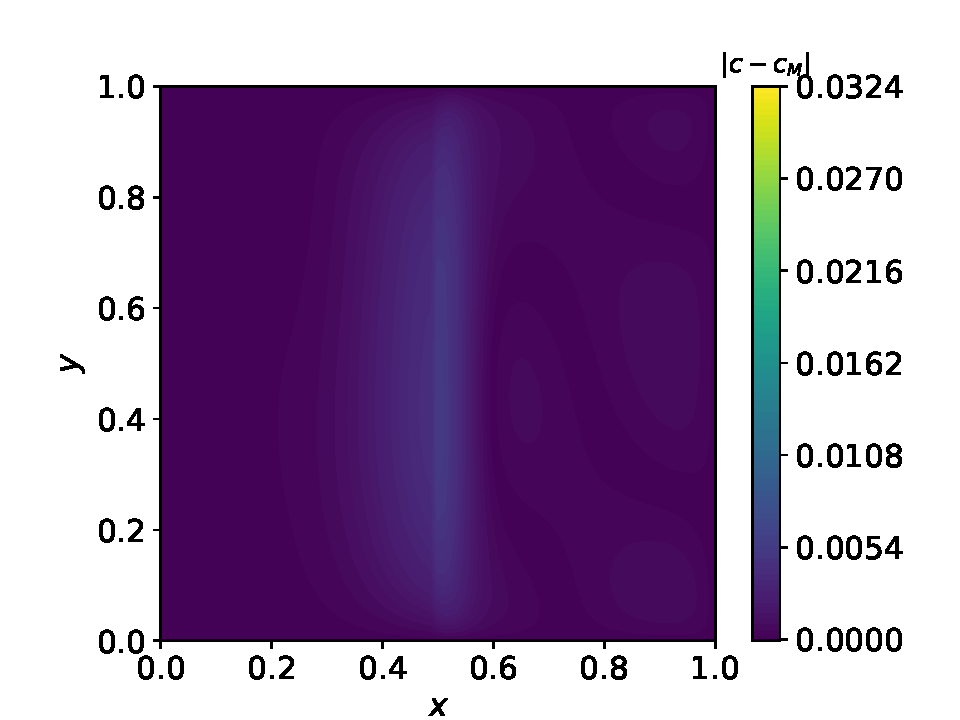
\includegraphics[width=\linewidth]{Figures/Chapter3/monoblocks/interface_condition/diff_t0.06.pdf}
        \caption{Absolute difference}
    \end{subfigure}
    \caption{Comparison of concentration fields simulated by FESTIM with manufactured solutions}
    \label{fig: results MMS}
\end{figure*}


\subsubsection{Heat transfer (MMS)}

% why not use a complex geometry? like an elbow

The heat transfer module in FESTIM can also be verified using the method of manufactured solutions.

Let us choose the following test problem on a elbow domain $\Omega = [0, 1] \times [0, 0.5] \cup [0, 0.5] \times [0.5, 1]$ with the manufactured solution $T_D(x, y) = \sin(\omega \pi x) \sin(\omega \pi y)$.

\begin{align}
    \nabla \cdot \lambda \nabla T &= -f \\
    T &= T_D \text{  on  } y \in [0, 1] \\
    -\lambda \nabla T \cdot \mathbf{n} &= -\lambda \nabla T_D \cdot \mathbf{n} \text{  on  other surfaces} \\
    \lambda(x, y) &= 2 + T_D^2 \\
\end{align}

The source term $f$ is therefore:
\begin{align}
    f &= 2 \pi^{2} \omega^{2} f_0 \sin{\left (\pi \omega x \right )} \sin{\left (\pi \omega y \right )} \\
    f_0 &= \left(3 f_1 f_2 - f_1 - f_2 + 2\right) \\
    f_1 &= \sin^{2}{\left (\pi \omega x \right )} \\
    f_2 &= \sin^{2}{\left (\pi \omega y \right )} \\
\end{align}

The computed FESTIM solution is extremely similar to the exact solution (see Figure \ref{fig: results MMS heat transfer}).
It is also possible to compute the L2-error for several number of cell divisions in the x and y directions $N$ to ensure the error decreases as a power law of $N$.
Moreover, the L2-error (the exponent of the power law) should vary as $h^{d+1}$ where $h=1/N$ and $d$ is the polynomial degree of the elements.
This was verified for P1 and P3 elements and a super-convergence rate was observed for the P2 elements (see Figure \ref{fig: convergence rates heat transfer}).

\begin{figure*}
    \centering
    \begin{subfigure}{0.5\linewidth}
        \centering
        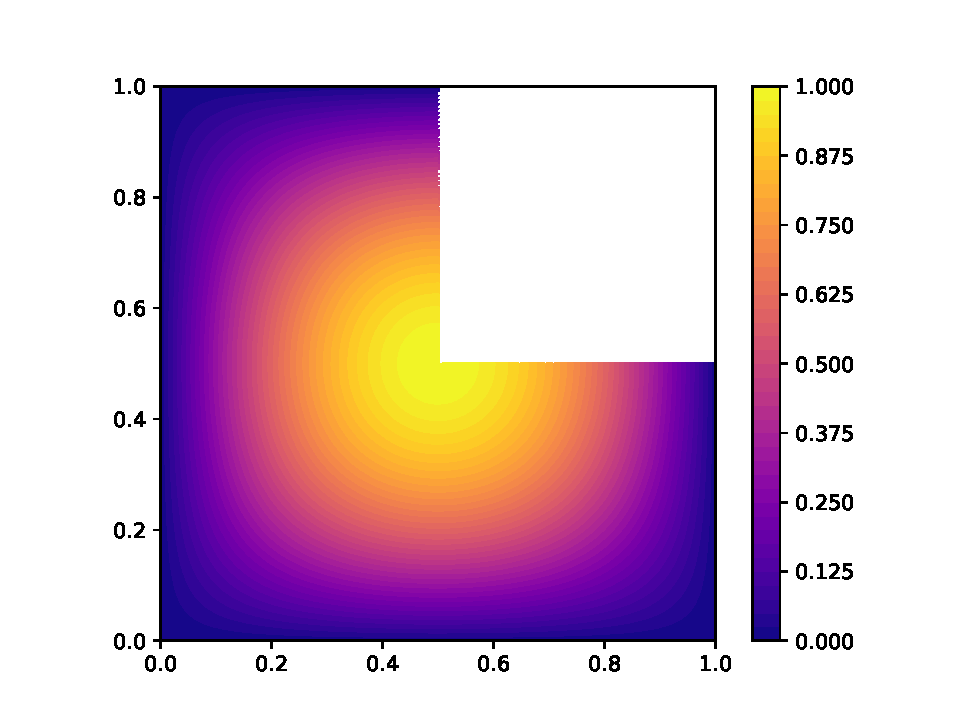
\includegraphics[width=\linewidth]{Figures/Chapter2/T.pdf}
        \caption{Computed temperature $N=64$}
    \end{subfigure}%
    \begin{subfigure}{0.5\linewidth}
        \centering
        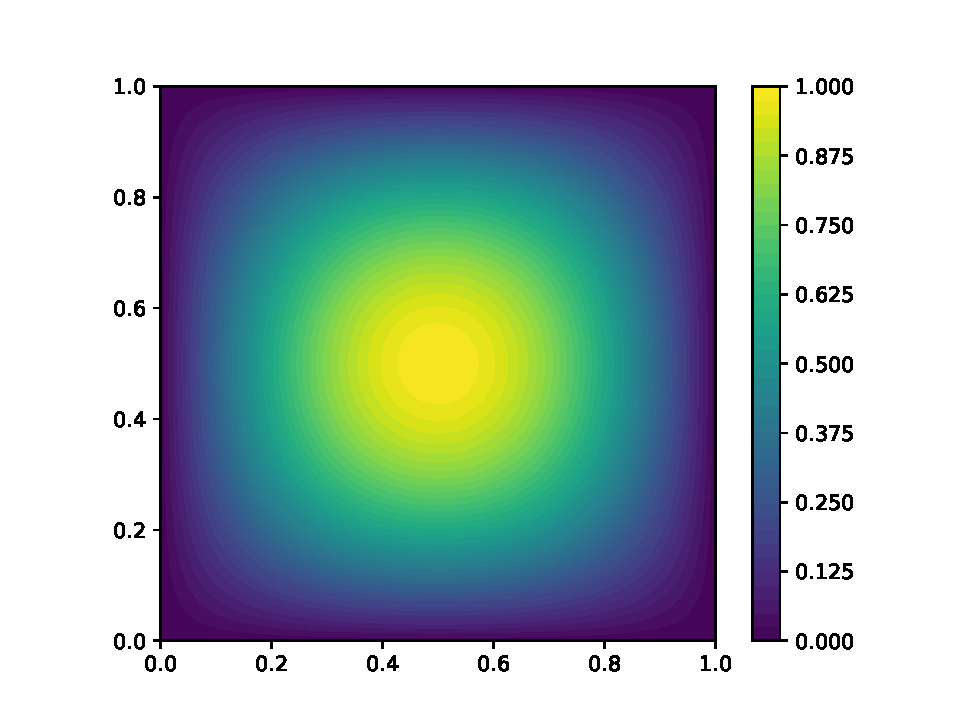
\includegraphics[width=\linewidth]{Figures/Chapter2/T_exact.pdf}
        \caption{Exact temperature}
    \end{subfigure}

    \caption{Verification of the heat transfer module in FESTIM}
    \label{fig: results MMS heat transfer}
\end{figure*}

\begin{figure}
    \centering
    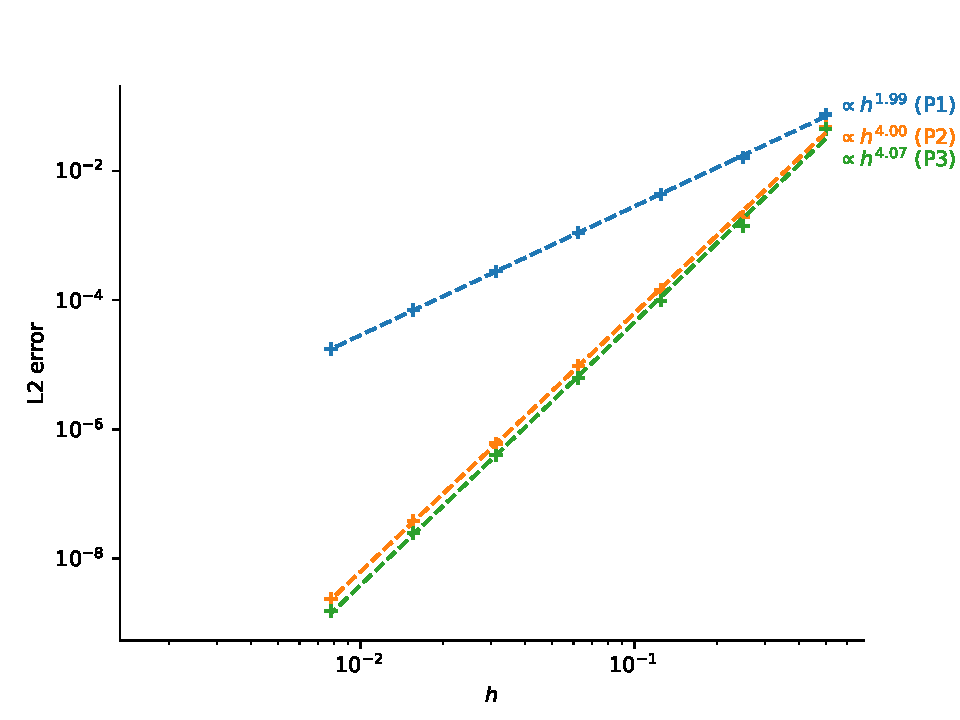
\includegraphics[width=\linewidth]{Figures/Chapter2/convergence_rate_heat_transfer.pdf}
    \caption{Convergence rates}
    \label{fig: convergence rates heat transfer}
\end{figure}



\subsection{Experimental validation}

Now that the code has been verified and solves the governing equations correctly, experimental validation is still required to check that these equations actually represent real life processes.
A very good example of real life experiments that can be reproduced are Thermo-Desorption Spectroscopy (TDS) experiments also called Thermally Programmed Desorption (TPD) experiments.
The principle of such experiments is to load small samples with H isotopes (H, D, or T) - either with a gas infusion or via plasma implantation - and heat it up to different temperatures to desorb the trapped H.
By measuring the outgassing flux of particles throughout the time of the experiment, desorption spectra are obtained.
These spectra often exhibit several peaks and each peak correspond to a kind of trap.

This technique is therefore employed to characterise materials and determine what kind of defects can be found in them. 
It is also a very good application case for experimental validation of the H transport model.

This section explains the technique that was employed to easily reproduce these TDS experiments.
Several application cases will also be shown on W, Al, EUROFER, and Be.

\subsubsection{Methodology} \label{methodology}
Fitting experimental data by manually tweaking parameters as in \sidecite{yu_deuterium_2019, hodille_macroscopic_2015} can be really time-consuming, sometimes days in some cases.
Moreover, some possible solutions in the parameter space might be missed by the user.
The goal of this study is to automate the parametric optimisation process by embedding FESTIM in a minimisation algorithm.

As in manual fitting, the parametric optimisation problem is solved by minimising a function representing the residual between simulated results and some reference data.
This function $f$ is called \textit{cost function}.
Considering fitting one or several TDS spectra (in order to identify for instance trapping parameters or diffusion coefficients), $f$ can simply be the mean absolute error described in Equation \ref{eq:cost function} representing the residual between the simulated spectrum and the experimental reference: 

\begin{equation}
    f(\textbf{x})=\frac{\sum_{i=0}^{N}  \alpha_i(T_i)\left| d_{i}-d_{\mathrm{sim}}\right|}{\sum_{i=0}^{N}  \alpha_i(T_i)}
    \label{eq:cost function}
\end{equation}

where \textbf{x} is the set of parameters used for the simulation, $d_\mathrm{sim}$ are the values of the simulated spectrum, $N$ is the number of experimental points $(T_i, d_i)$.
In Equation \ref{eq:cost function}, $f(\textbf{x})$ can be weighted by coefficients $\alpha_i$ in order to have a better fit on specific regions of the spectrum.
%Note that this cost function could as well be a root mean square error or any type of residual.

The parametric optimisation problem can now be solved by finding the minimum of the cost function $f$.
The global optimisation routine is illustrated on Figure \ref{fig:diagramm}.
\begin{figure}
    \centering
    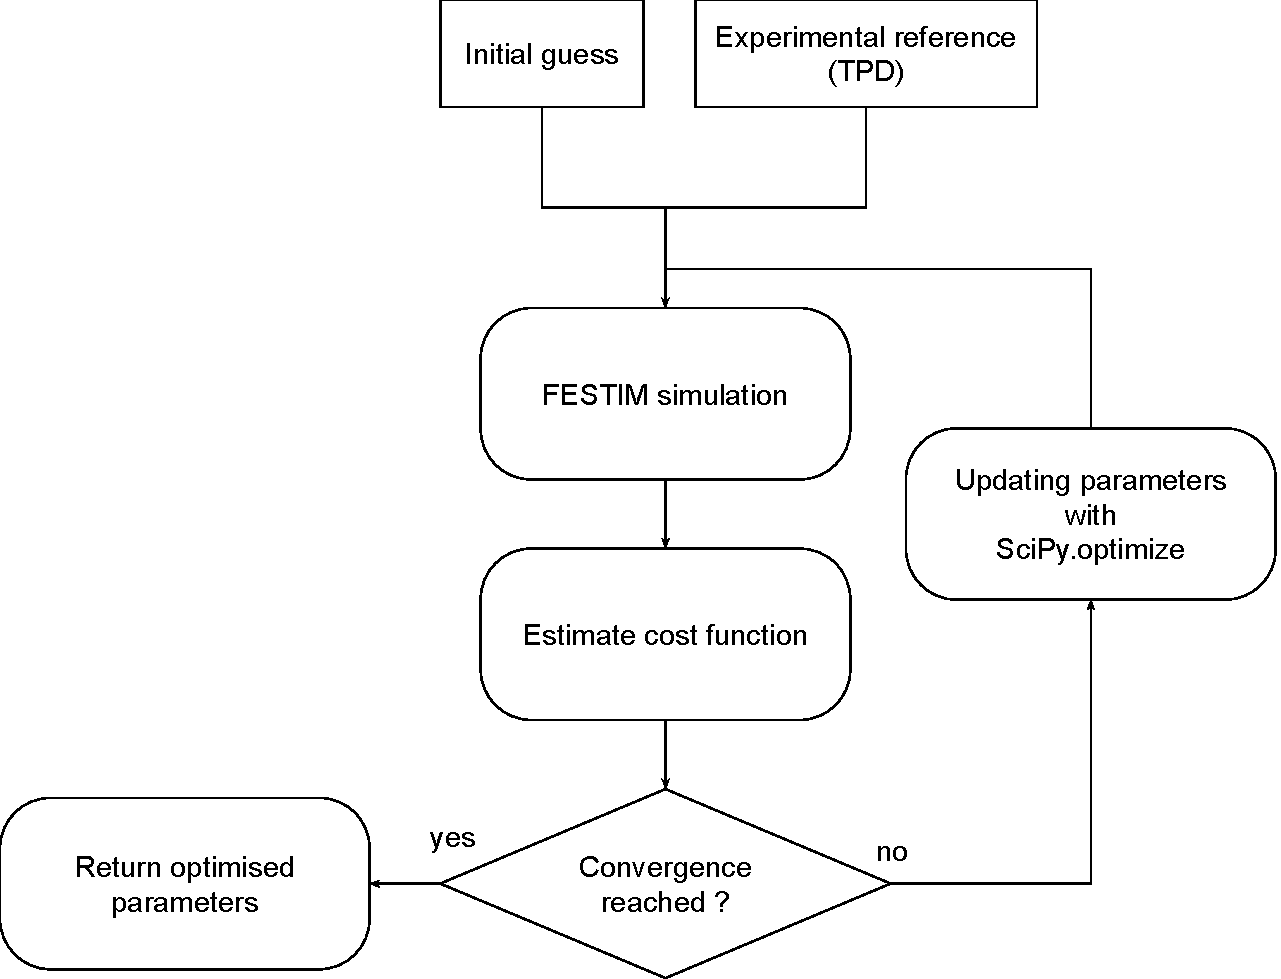
\includegraphics[width=\linewidth]{Figures/Chapter3/Parametric_optimisation/algorithm diagram.pdf}
    \caption{Diagram of the embedding of FESTIM within a parametric optimisation routine based on SciPy \cite{virtanen_scipy_2020}}
    \label{fig:diagramm}
\end{figure}

A comparative study of the several optimisation algorithms which can be employed is made in Section \ref{optimisation algorithms}.
These algorithms require the user to give an initial set of parameters called \textit{initial guess} and evaluate the cost function with several parameters sets until the convergence criterion is reached.
As in \sidecite{drexler_model-based_2019}, the Python package SciPy \sidecite{virtanen_scipy_2020} will be employed.

% \subsubsection{Optimisation algorithms} \label{optimisation algorithms}
Four minimisation algorithms have been benchmarked against a test case.
In the following example an experimental TDS spectrum from Ogorodnikova \textit{et al.} \sidecite{ogorodnikova_deuterium_2003} will be fitted and materials properties such as trap density and detrapping energy will be identified.
For this example case, two intrinsic traps and one extrinsic trap are set.
The only free parameters are $E_1$ and $n_1$, respectively the detrapping energy and density of trap 1.
The other parameters are constrained and described in \sidecite{delaporte-mathurin_finite_2019}.
The cost function $f$ has been plotted on Figure \ref{fig:cost function} as function of $E_1$ and $n_1$.

\begin{figure*} [ht]
    \centering
        \begin{subfigure}[t]{0.5\linewidth}
            \centering
            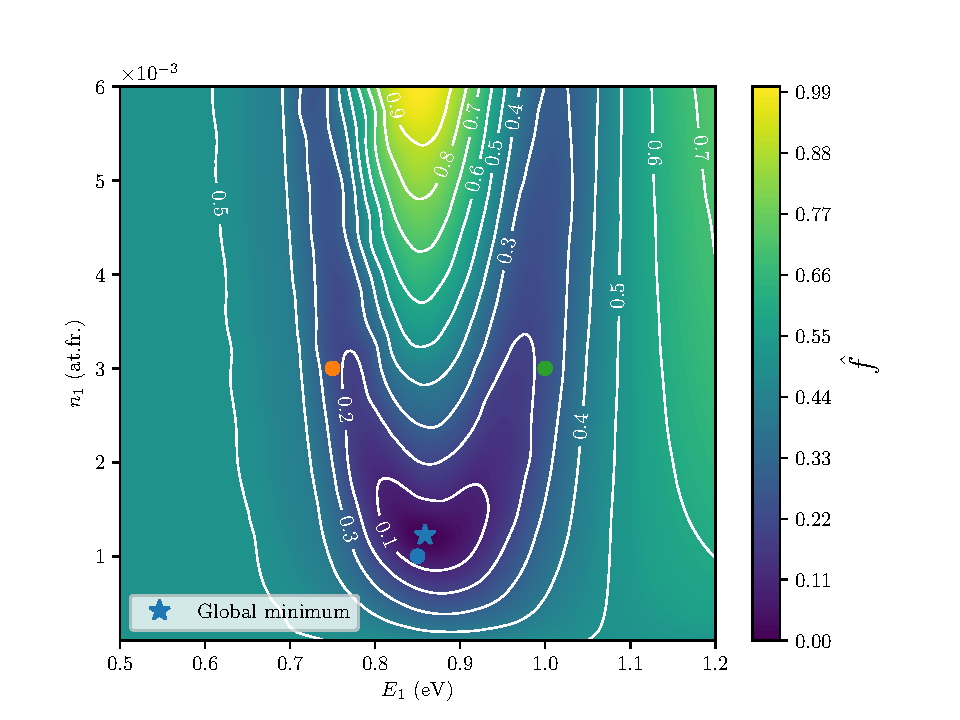
\includegraphics[width=\linewidth]{Figures/Chapter3/Parametric_optimisation/cost_function_2D.pdf}
            \caption{Normalised cost function}
            \label{fig:2D}
        \end{subfigure}%
        \begin{subfigure}[t]{0.5\linewidth}
            \centering
            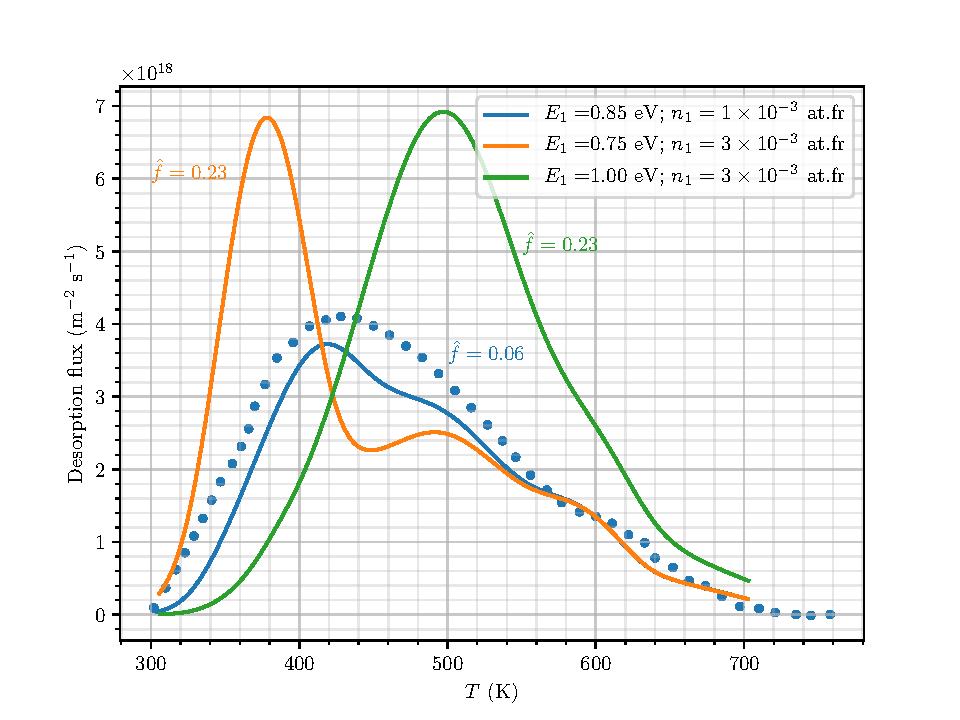
\includegraphics[width=\linewidth]{Figures/Chapter3/Parametric_optimisation/points_on_cost_function.pdf}
            \caption{Corresponding simulated TDS spectra}
            \label{fig:corresponding spectra}
        \end{subfigure}%
    \caption{Normalised cost function $\hat{f} = (f - \min{f})/(\max{f}-\min{f})$ as function of $E_1$ (\si{eV}) and $n_1$ (\si{at.fr.}) with global minimum located at $(\SI{0.86}{eV}, \SI{1.2e-3}{at.fr.})$.}
    \label{fig:cost function}
\end{figure*}

In this case, when only 2 free parameters are set the cost function has only one minimum (it is not necessarily the case for higher dimension optimisation problems).
However, if one fixes the trap density $n_1$ above $\approx \SI{2e-3}{at.fr.}$, the cost function has two local minima which can lead the optimisation routine to converged to a non-global minimum.
Moreover, $f$ is smooth and quadratic around its minimum located at $(E_1, n_1) = (\SI{0.86}{eV}, \SI{1.2e-3}{at.fr.})$.
For detrapping energies below \SI{0.6}{eV} and/or densities below \SI{0.5e-3}{at.fr}, the cost function is constant.
This is because for these values, the contribution of this trapping site to the TDS spectrum is zero either because the density is close to zero, or because the energy is too low for these traps to be filled at the implantation temperature of \SI{300}{K}.
Variations in these regions do not modify the simulated spectrum and thus do not modify the cost function value.

\begin{figure} [ht]
    \centering
    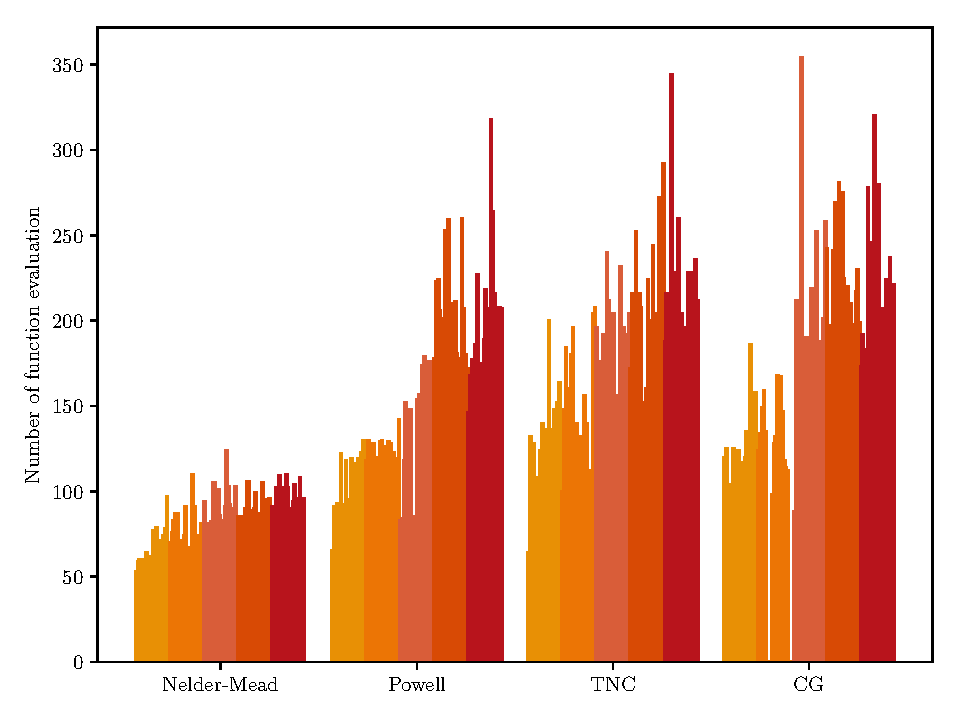
\includegraphics[width=\linewidth]{Figures/Chapter3/Parametric_optimisation/algorithms_perfs.pdf}
    \caption{Number of cost function evaluations required to converge towards the global minimum with 100 different initial guesses sorted by distance to the global minimum for several minimisation algorithms. Each cost function evaluation takes \SI{20}{s} to compute. White stripes correspond to initial guesses for which the algorithm did not converge to the global minimum.}
    \label{fig:algos perfs}
\end{figure}


Four different optimisation algorithms are being compared: 
Nelder-Mead (also called the simplex method), Powell, Truncated Newton method (TNC) and Conjugate Gradient (CG).
Thorough descriptions of these algorithms would be beyond the scope of this study but can be found in \sidecite{nocedal_numerical_2006}.
The performances of these algorithms have been compared with 100 different initial guesses randomly distributed on the $(E_1,n_1)$ plane and are shown on Figure \ref{fig:algos perfs}.
It appears that the CG algorithm is less robust since for some cases it didn't converge towards the global minimum (see white bands on Figure \ref{fig:algos perfs}).
Nelder-Mead algorithm appears to be the most efficient with initial guesses both close and far from the global minimum since the number of cost function evaluations ranges from 50 to 100 whereas other algorithms require more than 100.
This can be explained by the fact that Nelder-Mead is a derivative-free algorithm whereas TNC (Truncated Newton method) and CG algorithms need on the other hand to compute first order derivatives thus increasing the number of function evaluations.
This will be even more true when increasing the number of free parameters since the derivative will become more costly to compute.

It is worth noting that the Nelder-Mead algorithm is an unconstrained method.
If constraints or bounds are needed, TNC might be a more suitable choice.

Though in the following, the Nelder-Mead algorithm will be employed.


% \subsubsection{Results} \label{results}

% \subsection{Applications}

The fitting procedure has been employed to reproduce thermo-desorption experiments performed on Tungsten, EUROFER, Aluminium and Beryllium.


\subsubsection{Tungsten}

The TPD spectrum measured by Ogorodnikova \textit{et al} \sidecite{ogorodnikova_deuterium_2003} has been reproduced by setting all traps parameters as free parameters.
The fitting procedure has been run for several numbers of traps as shown on Figure \ref{fig:number of traps comparison}.
It is clear that setting only one trap is not sufficient to reproduce the experimental data.
The two traps case shows better results but also has a discrepancy near \SI{600}{K}.
This discrepancy is removed when setting a third extrinsic trap to the simulation.

For this last case, the five free parameters are the detrapping energies $E_{p, 1}$, $E_{p, 2}$, $E_{p, 3}$ and densities $n_1$, $n_2$ (the third trapping site being created during the implantation, for which the creation parameters are not part of the free parameters and taken from \cite{ogorodnikova_deuterium_2003} or \sidecite{hodille_macroscopic_2015}).
This optimisation case is therefore a 5D optimisation problem.
Every other parameter is taken from \cite{hodille_macroscopic_2015}.
The resulting fit is shown on Figure \ref{fig:5D TPD} alongside with the contribution of each trap to the total spectrum.
% (1 trap [ 0.88368005  1.44347635] 2 traps [ 0.83582125  1.23768655  0.98708714  6.85457283])
\begin{figure*} [ht]
    \centering
        \begin{subfigure}[t]{0.5\linewidth}
            \centering
            \captionsetup{width=.9\linewidth}
            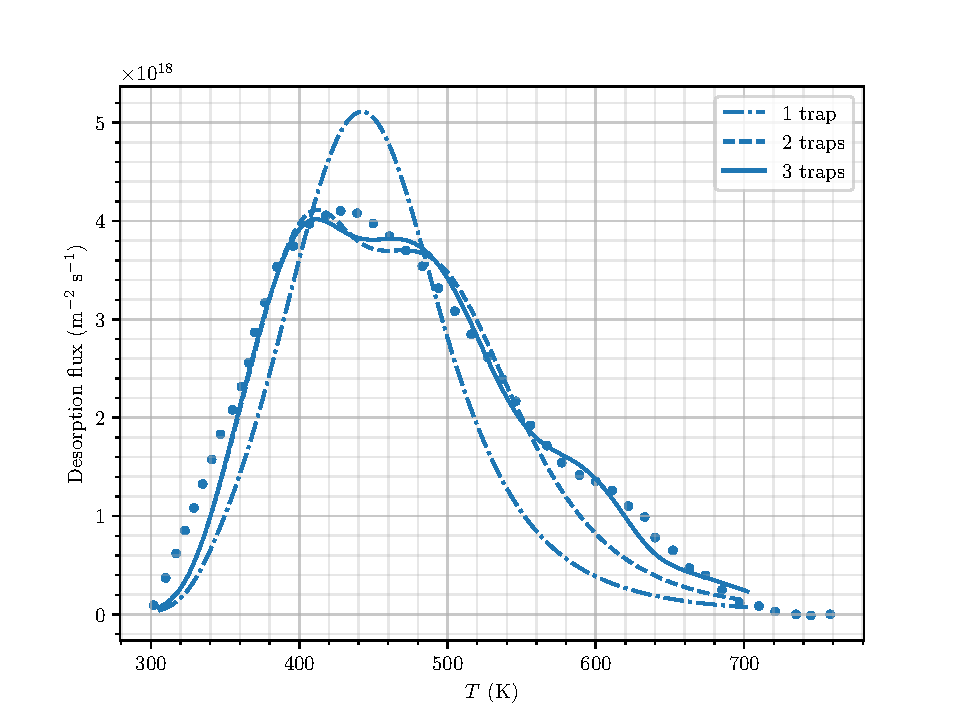
\includegraphics[width=\linewidth]{Figures/Chapter3/Parametric_optimisation/number_of_traps.pdf}
            \caption{Comparison of the resulting fit with several numbers of traps in the simulation.}
            \label{fig:number of traps comparison}
        \end{subfigure}%
        \begin{subfigure}[t]{0.5\linewidth}
            \centering
            \captionsetup{width=.9\linewidth}
            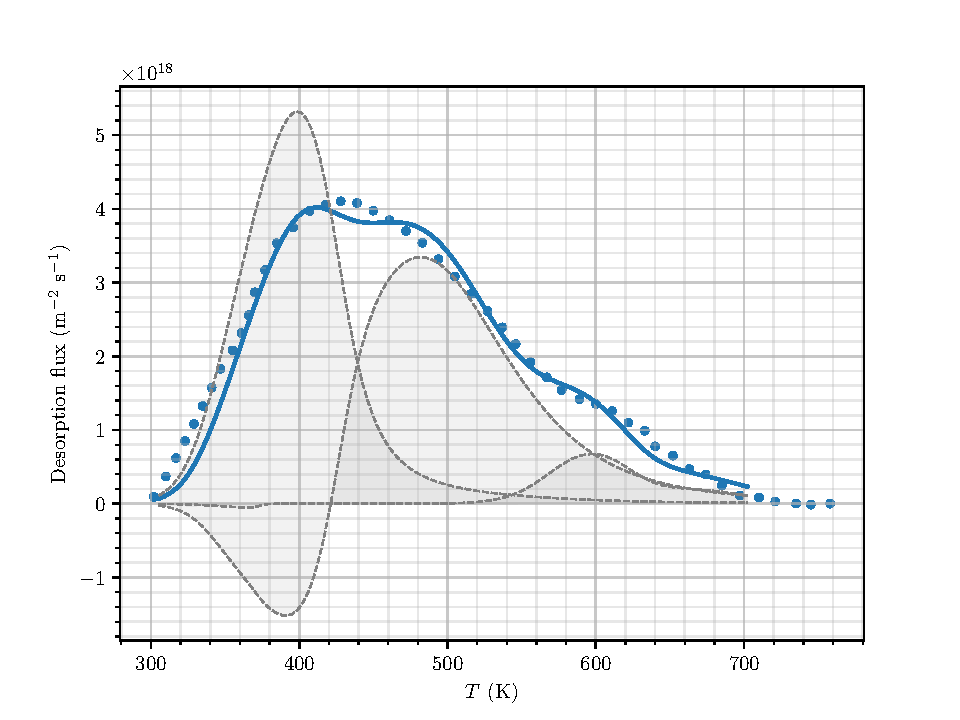
\includegraphics[width=\linewidth]{Figures/Chapter3/Parametric_optimisation/Ogorodnikova_5D.pdf}
            \caption{Identified by the fitting procedure with $E_1 = \SI{0.83}{eV}$, $E_2 = \SI{0.97}{eV}$, $E_3 = \SI{1.51}{eV}$, $n_1 = \SI{1.18e-3}{at.fr.}$ and \newline $n_2 = \SI{7.22e-4}{at.fr.}$.  Dashed lines correspond to the temporal evolution of each trapping population's inventory.}
            \label{fig:5D TPD}
        \end{subfigure}%
    \caption{Fitting TPD spectrum performed on Tungsten by Ogorodnikova \textit{et  al} \cite{ogorodnikova_deuterium_2003}. Dots correspond to experimental data.}
    \label{fig:TPD ogorodnikova}
\end{figure*}
The identified parameters are similar to the ones found by Hodille \textit{et al.} in \cite{hodille_macroscopic_2015}.
The total fitting procedure took a few hundred of cost function evaluations.
One single cost function evaluation "costing" less than \SI{20}{s} to compute (for that specific case), the total procedure lasted less than \SI{3}{h}.

\subsubsection{EUROFER}

Hollingsworth \textit{et al} performed thermo-desorption on pre-damaged EUROFER at several damage levels \sidecite{hollingsworth_comparative_2019}.
Three spectra with similar exposure conditions have been fitted with one trapping site (since only one peak appears on the spectra) as shown on Figure \ref{fig:TPD EUROFER}.

\begin{figure} [ht]
    \centering
    \includegraphics[width=\linewidth]{Figures/Chapter3/Parametric_optimisation/EUROFER_hollingsworth.pdf}
    \caption{TPD spectra of damaged EUROFER \cite{hollingsworth_comparative_2019}. Fitted with one trapping site (solid line) $E=\SI{1.06}{eV}$ and densities of \SI{8.9e-3}{at.fr}, \SI{2.8e-2}{at.fr} and \SI{5.0e-2}{at.fr} for \SI{0}{dpa}, \SI{0.01}{dpa} and \SI{0.1}{dpa}, respectively. Dashed lines correspond to optimisations with an unweighted cost function. Dots correspond to experimental data.}
    \label{fig:TPD EUROFER}
\end{figure}

To put the emphasis on peaks, a weighting factor of 10 has been applied for $T \in [\SI{445}{K}, \SI{492}{K}]$.
Not applying this factor near the peak region results in a closer fit in other regions but a higher peak value.
The identified trap energy is $E_p$ \SI{1.06}{eV} for all spectra whereas the trap density $n$ is \SI{8.9e-3}{at.fr} for the undamaged sample, \SI{2.8e-2}{at.fr} for \SI{0.01}{dpa} and \newline \SI{5.0e-2}{at.fr} for \SI{0.1}{dpa}.
For all simulations the attempt frequency $p_0$ is \SI{1e13}{s^{-1}} and the diffusion coefficient is taken from \sidecite{esteban_hydrogen_2007}.

The total fitting procedure took less than two hours for fitting the three spectra.
A more thorough study of these experiments could involve constraining the algorithm with profilometry data obtained by Hollingsworth \textit{et al} \cite{hollingsworth_comparative_2019}.
Indeed, having a non-homogeneous trapping site distribution could help having a better fit of both the profilometry data and the TPD spectra. 

\subsubsection{Aluminium}

The experiment performed on Aluminium by Quiros \textit{et al} \sidecite{quiros_blistering_2019, quiros_blister_2017} has also been reproduced with FESTIM.

Only one trap has been set in the simulation and its energy $E_p$ and density $n$ are set as free parameters.
Every other parameters are fixed and taken from \cite{quiros_blister_2017, quiros_blistering_2019}.
The resulting simulated TPD spectrum is shown on Figure \ref{fig:TPD alu}.
\begin{figure} [ht]
    \centering
    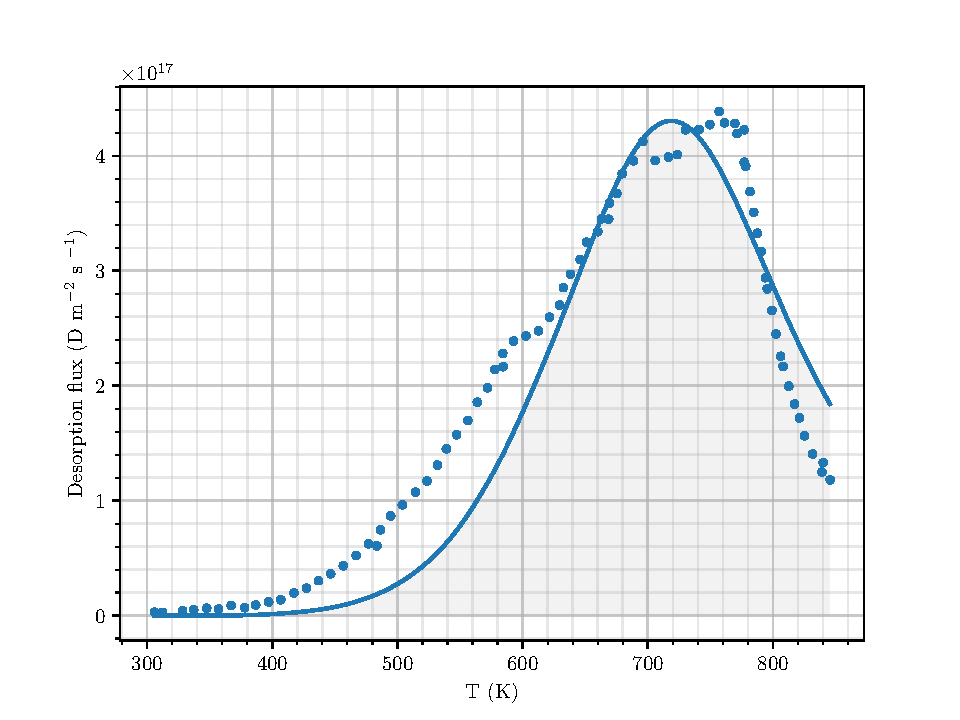
\includegraphics[width=\linewidth]{Figures/Chapter3/Parametric_optimisation/alu_quiros.pdf}
    \caption{TPD spectrum of aluminium exposed to \SI{3e23}{H.m^{-2}} at \SI{618}{K} \cite{quiros_blister_2017, quiros_blistering_2019}. Fitted with one trapping site $n = \SI{1.8e-2}{at.fr.}$ and $E =\SI{1.1}{eV}$. Dots correspond to experimental data. Dashed lines correspond to the temporal evolution of each trapping population's inventory.}
    \label{fig:TPD alu}
\end{figure}


The identified parameters are $n = \SI{1.8e-2}{at.fr.}$ and $E =\SI{1.1}{eV}$.
The trapping sites density is significantly higher than the one described in \cite{quiros_blister_2017}.
However, the TPD spectrum obtained with this procedure better fits the experimental data since the one obtained by Quiros \textit{et al} requires a 10-fold increase.
The fitting procedure took less than a hundred cost function evaluations, which corresponds in total to a few dozens of minutes.

\subsubsection{Beryllium}
Be co-deposition experiments performed by Baldwin \textit{et al} \sidecite{baldwin_experimental_2014} were reproduced with FESTIM using this optimisation technique.
In this experiment, a \SI{1}{\micro m} thick Be-D layer is grown on Tungsten at \SI{330}{K}. 
Following the strategy proposed by Baldwin \textit{et al}, only the thermo-desorption phase has been simulated with two trapping sites with homogeneously distributed densities and with initial occupancies $f_i$.
There are therefore three free parameters per trap (energy, density and initial occupancy) which makes this optimisation problem 6D.
It is assumed that the surface flux is the net balance between incoming flux from the chamber (very low since the pressure is $\SI{1}{\micro Pa}$) and the molecular recombination flux.
All the other parameters are described in \cite{baldwin_experimental_2014}.

The resulting optimised TPD spectrum is shown on Figure \ref{fig:tpd baldwin}.
The optimised parameters are $E_{p, 1} = \SI{0.75}{eV}$, $n_1 = \SI{1.09e-1}{at.fr.}$, $f_1=0.73$, $E_{p, 2} = \SI{0.93}{eV}$, \newline ${n_2 = \SI{3.40e-2}{at.fr.}}$, $f_2=0.28$.
These values are in agreement with the ones found by Baldwin \textit{et al} \cite{baldwin_experimental_2014} and took only a few of minutes to compute since the implantation phase was not simulated.

\begin{figure}
    \centering
    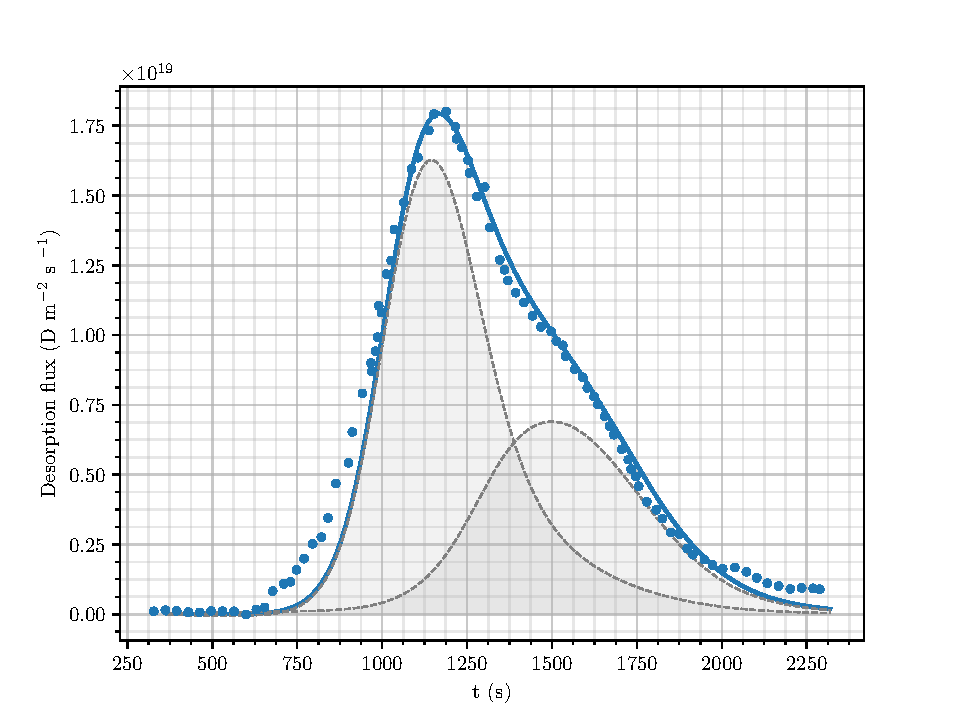
\includegraphics[width=\linewidth]{Figures/Chapter3/Parametric_optimisation/baldwin_be.pdf}
    \caption{TPD spectrum of co-deposited Be-D \cite{baldwin_experimental_2014} simulated with two trapping sites. Dots correspond to experimental data.}
    \label{fig:tpd baldwin}
\end{figure}

\subsubsection{Discussion}

Even though an automated technique is proposed, the user still has some choices to make in order to ensure the credibility of the fitted spectrum.
As shown on Figure \ref{fig:TPD EUROFER}, weighting the cost function near regions of interest will result in a better fit in these regions.
Users should also be aware of the number of traps the data is being fitted with.
As shown on Figure \ref{fig:number of traps comparison} too few traps in the simulation will not result in a satisfactory fit (even though the optimisation routine will converge to an optimised solution).
Moreover, as shown on Figure \ref{fig:hurley_comparison}, one single TPD spectrum can be reproduced with several traps of different energies and densities.
This means that the cost function with several traps as free parameters can have several local minima of very similar values.
Adding traps to an optimisation problem can also help having a better fit of the experimental data in some cases.
But artificially adding more and more traps is not necessarily realistic and could lead to misinterpretation of the results.

\begin{figure}[ht]
    \centering
    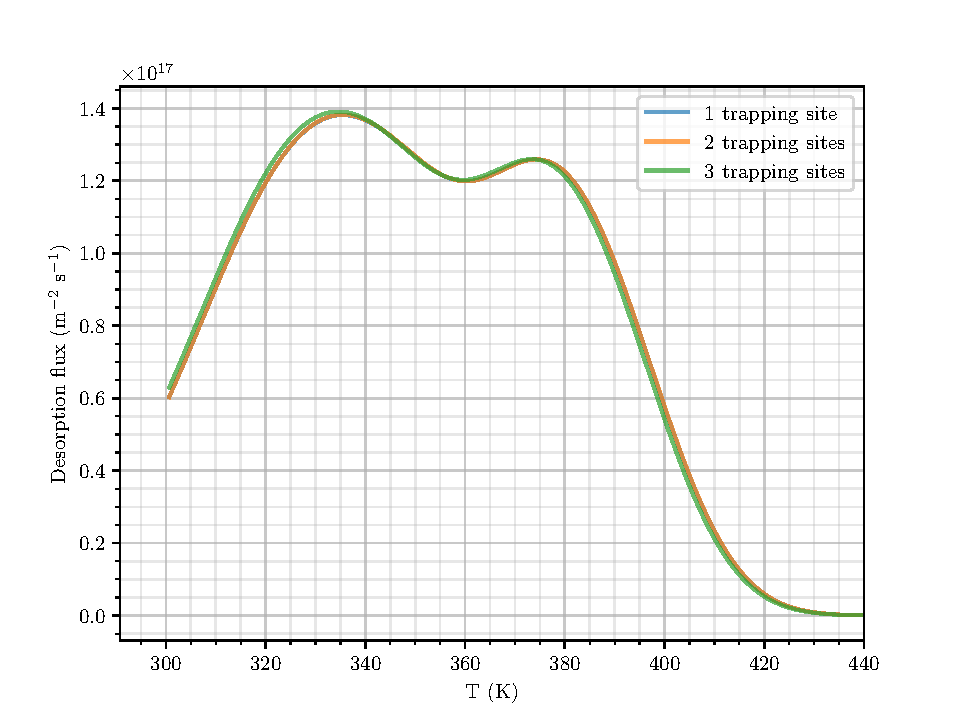
\includegraphics[width=\linewidth]{Figures/Chapter3/Parametric_optimisation/hurley_comparison.pdf}
    \caption{TPD spectrum reproduced with several sets of parameters showing the existence of several solutions to a single optimisation problem.}
    \label{fig:hurley_comparison}
\end{figure}

In the first case with only one trapping site, as described by Hurley \textit{et al} in \sidecite{hurley_numerical_2015}, the binding energy is \SI{0.55}{eV} and the trap density is \SI{2.08e24}{m^{-3}}.
The appearance of two peaks is due to the desorption on different sides of the sample as explained in \cite{hurley_numerical_2015}.
In the second case, the curve as been reproduced with two trapping sites which energies and densities are respectively \SI{0.51}{eV} and \SI{0.57}{eV} and \SI{2.02e24}{m^{-3}} and \SI{2.12e24}{m^{-3}}.
In the third case, it has been reproduced with three trapping sites which energies and densities are respectively \SI{0.55}{eV}, \SI{0.38}{eV} and \SI{0.51}{eV} and \SI{2.12e24}{m^{-3}}, \SI{2.26e24}{m^{-3}} and \newline \SI{2.13e24}{m^{-3}}.

This example illustrates how a single spectrum can be simulated with several sets of parameters by varying the number of traps in the simulation.
One way to avoid this from happening is to have a set of experiments with varying parameters such as the implantation temperature, the heating ramp, the fluence, dwelling time before TPD, etc.


\section{Summary}
\setchapterimage[3cm]{seaside}
\chapter{H transport in PFCs} \label{Chapter3}

\section{Introduction}

\section{Validation \& Verification}
\subsection{Experimental validation}
In order to further validate the model, the laboratory experiments from Ogorodnikova \textit{et al} \cite{ogorodnikova_deuterium_2003} are simulated.
We choose these particular experiments as it has already been simulated several times in \sidecite{ogorodnikova_deuterium_2003,hodille_macroscopic_2015,bonnin_rate_2015,benannoune_numerical_2019}.
Therefore, this simulation can be used as a benchmark case for FESTIM.\\
In this experiment, after deuterium (D) implantation in hot-rolled tungsten (W), Temperature Programmed Desorption (TPD) is performed.
TPD consists in heating the sample with a well controlled temperature ramp and measure with a mass spectrometer the evolution of the amount of desorbed particles with respect to temperature.
This results in a TPD spectrum.
In order to reproduce this spectrum, three phases are simulated.

The first one is the implantation phase where the source term in Equation \ref{eq:mobile} is $S_{ext} = (1-r) \cdot \varphi \cdot f(x)$, $r$ being the reflection coefficient (\textit{i.e.} the proportion of particles which are reflected from the surface to the plasma), $\varphi$ the incident ion flux in $\si{m^{-2}.s^{-1}}$ and $f(x)$ a Gaussian distribution with $R_p$ its mean value and $\sigma$ its width.
The parameters of $f(x)$ are determined with the software SRIM \sidecite{ziegler_srim_2010}.
This phase lasts $t_\mathrm{imp}$ and the temperature is $T = T_\mathrm{imp}$.\\
The second phase is the resting period where the source is turned off (\textit{i.e.} $S_{ext} = 0$) for a time $t_\mathrm{rest}$ at $T = T_\mathrm{rest}$.\\
Finally, the last period is the TPD where temperature is increased linearly with a given heating ramp $\beta$.\\
In order to fit the experimental results, three traps are needed: two intrinsic traps and one extrinsic trap to account for the creation of ion-induced defects during the implantation.
Extrinsic traps can be created by either supersaturation of HIs in the implantation range $f(x)$ creating monovacancies \sidecite{sun_critical_2014, fernandez_hydrogen_2015, ohsawa_thermodynamics_2015, kato_super-saturated_2015,hodille_hydrogen_2018}, that can lead to vacancy clusters and bubbles \sidecite{ogorodnikova_deuterium_2003, condon_hydrogen_1993} or local stress field \sidecite{poon_flux_2002, alimov_depth_2005}.
According to \sidecite{hodille_hydrogen_2018}, mono-vacancies can be created in the implantation zone when W is exposed to D ion flux if the flux is higher than a threshold limit for a given temperature.
At the temperature of the considered experiment (300 K), the threshold flux is ~$10^{18}$ $\: \si{m^{-2}s^{-1}}$ which is lower than the flux in the experiment (see Table \ref{tab:parameters validation}).


The evolution of the extrinsic trap density is given by Equation \ref{eq:extrinsic trap}.
 
\begin{equation}
    \begin{split}
        \frac{dn_3}{dt}  = (1-r)\: \varphi\:  \bigg[ & \left(1-\frac{n_3}{n_{3a_\mathrm{max}}}\right) \:\eta_a  \:f(x) \\  + &\left(1-\frac{n_3}{n_{3b_\mathrm{max}}}\right) \:\eta_b  \:\theta_{xp}(x) \bigg]
    \end{split}
    \label{eq:extrinsic trap}
\end{equation}
 
where $\theta_{xp}(x) = \frac{1}{x_p}\quad \forall x < x_p$, $\eta_a$ and $\eta_b$ are the rates of traps creation and ${n_{3a_\mathrm{max}}}$ and ${n_{3b_\mathrm{max}}}$ are their maximum values.
This formulation follows the one proposed in \sidecite{hodille_macroscopic_2015,bonnin_rate_2015} based on the expression of Ogorodnikova \textit{et al.} \sidecite{ogorodnikova_deuterium_2003}.

All the above parameters are presented in Table \ref{tab:parameters validation}. These parameters are in good agreement with those used in \sidecite{hodille_macroscopic_2015,bonnin_rate_2015,benannoune_numerical_2019}.
\begin{table} [ht]
    \centering
    \begin{tabular}{p{2.3cm} p{2cm} r}
        %\hline
        Parameter & Units & Value \\
        \hline
        \\
        $\rho_W$ & $\si{m^{-3}}$ &$6.3 \times 10^{28}$ \\
        $n_\mathrm{solute}$ & & $6 \:\rho_W$\\
        $n_1$ & & $1 \times 10 ^{-3} \rho_W$ \\
        $n_2$ &  & $4 \times 10 ^{-4} \rho_W$ \\
        $n_{3a_\mathrm{max}}$ & & $1 \times 10 ^{-1} \rho_W$ \\
        $n_{3b_\mathrm{max}}$ & & $1 \times 10 ^{-2} \rho_W$ \\
        \\
        $E_\mathrm{diff}$ & $\si{eV}$ & $0.39$ \\
        $E_1$ &  & $0.87$ \\
        $E_2$ &  & $1.00$ \\
        $E_3$ &  & $1.50$ \\
        \\
        $\eta_a$ & - & $6 \times 10 ^{-4}$ \\
        $\eta_b$ & - & $2 \times 10 ^{-4}$ \\
        \\
        $\lambda$ & $\si{m}$ & $110 \times 10 ^{-12}$  \\
        $x_p$ & & $1 \times 10 ^{-6}$ \\
        $R_p$ & & $4.5 \times 10^{-9}$ \\
        $\sigma$ & & $4.5 \times 10^{-9}$ \\
        \\
        $T_\mathrm{imp}$ & $\si{K}$ & 300 \\
        $T_\mathrm{rest}$ & & 300 \\
        \\
        $t_\mathrm{imp}$ & $\si{s}$ & 400 \\
        $t_\mathrm{rest}$ & & 50 \\
        \\
        $\nu_0$ & $\si{s^{-1}}$ & $10 ^{13}$ \\
        $\beta$ & $\si{K.s^{-1}}$ & 8 \\
        $D_0$ & $\si{m^2.s^{-1}}$ & $4.1 \times 10 ^{-7}$ \\
        $\varphi$ & $\si{m^{-2}.s^{-1}}$ & $2.5 \times 10 ^{19}$ \\
        $r$ & - & 0 \\
        \\
    \end{tabular}
    \caption{Parameters used for experimental validation}
    \label{tab:parameters validation}
\end{table}

The simulated TPD spectrum is represented on Figure \ref{fig:TPD spectrum}.
\begin{figure} [ht]
    \centering

    \begin{overpic}[width=1\linewidth]{"Figures/Chapter3/Comparaison exp-FESTIM"}
    \put(35,55){$\Bigg\uparrow$}
    \put(44.5,45){$\Bigg\uparrow$}
    \put(63.5,20){$\Bigg\uparrow$}
    \end{overpic}
    \caption{TPD spectrum simulated by FESTIM compared to experimental data of Ogorodnikova \textit{et al.} \cite{ogorodnikova_deuterium_2003}.}
    \label{fig:TPD spectrum}
\end{figure}

One can see that the spectra produced by FESTIM and by Ogorodnikova \textit{et al.} \sidecite{ogorodnikova_deuterium_2003} are in good agreement.
One peak can be distinguished at 450 K with two pronounced shoulders at 500 K and 620 K.
As denoted by the arrow in Figure \ref{fig:TPD spectrum}, the peak at 450 K corresponds to the detrapping from the low-energy high-concentration trap and the shoulders at 500 K and 620 K correspond to detrapping from 1.00 eV and 1.50 eV trap, respectively.
\subsection{Analytical verification}
\subsubsection{Analytical verification against a known solution} \label{analytical}

Although validation against experiments could show that FESTIM is able reproduce the data with a given set of parameters, objective verification against analytical solutions is first required to ensure that the governing Equations \ref{eq:mobile} and \ref{eq:trapped} are solved correctly.

For this verification case, a 1D slab is considered with a thickness $l$.
The concentration of mobile particles was set to $c_0$ on one side of the slab and set to zero on the other side.
Only one trap is considered in this case and its density $n_1$ is homogeneously distributed.

The trapping parameter $\zeta$ is defined in \sidecite{longhurst_verification_2005} as follow:
\begin{equation}
    \zeta = \frac{\lambda^2 \: n_\mathrm{solute} \: \nu_0}{D_0 \: n_1}\exp\bigg(\frac{E_\mathrm{diff} - E_1}{k_B \: T}\bigg) + \frac{c_m}{n_1}
\end{equation}

In our case, we choose the detrapping energy $E_1$, the concentration $c_0$ and the temperature $T$ so that $\zeta \gg \frac{c_m}{n_1}$.
This is known as the \textit{effective diffusivity regime} where the diffusion is almost identical to the case where there are no traps.
The coefficient $D$ is then replaced by an effective diffusion coefficient:
\begin{equation}
    D_\mathrm{eff} = \frac{D}{1+\frac{1}{\zeta}}
\end{equation}
The particle flux at the background surface is expressed in $\SI{}{H.m^{-2}.s^{-1}}$ and finally defined in \sidecite{longhurst_verification_2005} by:
\begin{equation}
    \varphi_H(t) = \frac{c_0 D}{l}\bigg[1+2\sum_{m=1}^{\infty}(-1)^m \exp\bigg(-m^2\frac{\pi^2 \:D_\mathrm{eff} \: t}{l^2}\bigg)\bigg]
\label{eq:flux analytical}
\end{equation}
All the parameters are defined in Table \ref{tab:parameters analytical verification}.
These parameters have been chosen for the sake of verification and do not necessarily represent realistic conditions as verification is a mathematical exercise.
\begin{table}
    \centering
    \begin{tabular}{p{2.3cm} p{2cm} r}
        Parameter & Units & Value \\
        \hline
        \\
        $\rho$ & $\si{m^{-3}}$ &$\SI{3.16e22}{}$ \\
        $n_1$ & & $\SI{1.00e-1}{} \rho$ \\
        $c_0$ & & $\SI{1.00e-4}{} \rho$\\
        $n_\mathrm{solute}$ & & $2 \:\rho$\\
        \\
        $E_1$ & $\si{eV}$ & $\SI{8.6e-3}{}$ \\
        $E_\mathrm{diff}$ & & $0$ \\
        \\
        $\lambda$ & $\si{m}$ & $\SI{3.16e-8}{}$  \\
        $l$ & & $\SI{5e-5}{}$\\
        \\
        $T$ & $\si{K}$ & 1000 \\
        \\
        $t_f$ & $\si{s}$ & \SI{e-8}{} \\
        $\nu_0$ & $\si{s^{-1}}$ & $\SI{e13}{}$ \\
        $D_0$ & $\si{m^2.s^{-1}}$ & $1$ \\
        \\
    \end{tabular}
    \caption{Parameters used for the analytical verification}
    \label{tab:parameters analytical verification}
\end{table}
One can notice on Figure \ref{fig:FESTIM vs analytical} that the numerical results are in good agreement with the analytical solution.
The maximum error between analytical and numerical solutions is calculated to be \SI{6.56e20}{H.m^{-2}.s^{-1}} with 50000 piecewise linear elements (P1) which corresponds to \SI{1}{\%} of the maximum value.
According to finite elements theory, this value will decrease with the stepsize and with the element size.
\begin{figure}
    \centering
    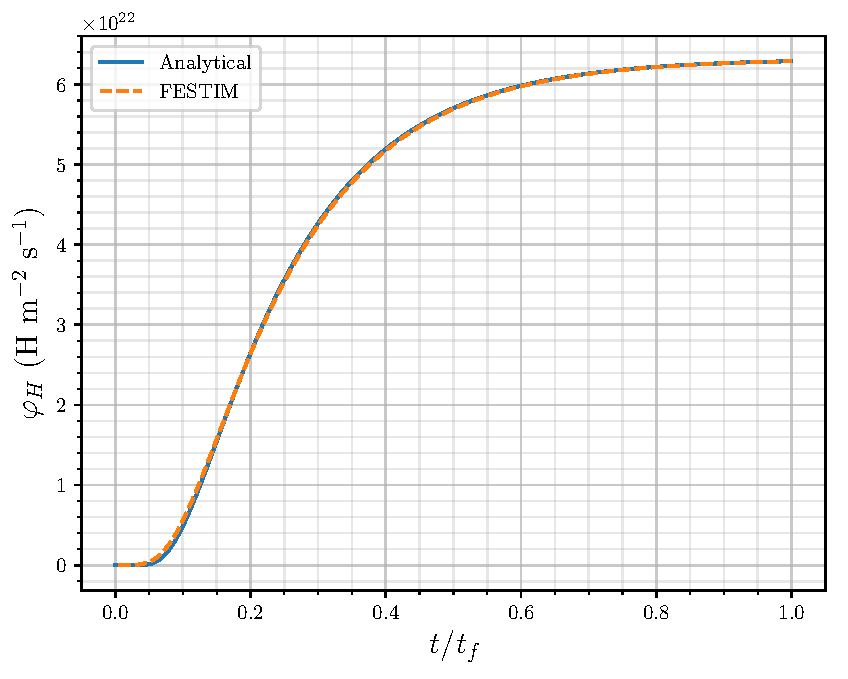
\includegraphics[width=\linewidth]{Figures/Chapter3/FESTIM_vs_analytical.pdf}
    \caption{Temporal evolution of the particle flux $\varphi_H$ ($t_f = \SI{e-8}{s}$)}
    \label{fig:FESTIM vs analytical}
\end{figure}
\subsubsection{Analytical verification using MMS} \label{mms}

To unravel the complexity of governing equations, the Method of Manufactured Solutions (MMS) is often used \sidecite{dudson_verification_2016, roache_code_2002}.
Manufactured solutions are exact solutions that have been modified with additional source terms.
The sets of source terms and boundary conditions obtained are then fed into FESTIM and the error is measured.


At this extent the following manufactured solutions are chosen:
\begin{equation}
    \begin{cases}
    c_{m_D} = 1 + x^2 + \sin(t) \\
    c_{{t,1}_D} = 1 + x^2 + \cos(t)
    \end{cases}
    \label{eq: manufactured solutions}
\end{equation}

By combining Equations \ref{eq:mobile}, \ref{eq:trapped} and \ref{eq: manufactured solutions}, one can obtain the following source terms:
\begin{equation}
    \begin{cases}
    f = \cos(t) - \sin(t) - 2D \\
    g_1 = \nu_1 c_{{t,1}_D} - \nu_m c_{m_D} ( n_1 - c_{{t,1}_D}) - \sin(t)
    \end{cases}
    \label{eq:sources}
\end{equation}

where $g_1$ is an additional source term in Equation \ref{eq:trapped}.
The Dirichlet boundary conditions for $c_m$ and $c_{t,1}$ are:

\begin{equation}
    \begin{cases}
    c_m = 1 + x^2 + \sin(t) \quad \text{on } \partial \Omega \\
    c_{t,1} = 1 + x^2 + \cos(t) \quad \text{on } \partial \Omega 
    \end{cases}
\end{equation}
where $\partial\Omega$ is the boundary of the domain.
Finally, initial values for $c_m$ and $c_{t,i}$ are:
\begin{equation}
    \begin{cases}
    c_m(t=0) = 1 + x^2 \\
    c_{t,1}(t=0) = 2 + x^2
    \end{cases}
\end{equation}
Once all these parameters are fed into FESTIM, one can easily compare the computed solution with the exact solution in Equation \ref{eq: manufactured solutions}.
The L2-norm $E_{c_m}$ can then be calculated as follow:
\begin{equation}
    E_{c_m} = \sqrt{\int_\Omega(c_{m_D} - c_m)^2dx}
\end{equation}
The evolution of $E_{c_m}$ as function of the element size $h$ is shown on Figure \ref{fig:error vs h}.
One can notice that $E_{c_m}$ increases as $A\cdot h^k$.
This is known as the \textit{asymptotic regime} and the coefficient $k$ is called the convergence rate.
$k$ typically tends to N+1 as $h$ approaches $0$, $N$ being the order of the finite elements.
In this simulation, $k$ approaches $2$ as expected since elements of order $1$ have been used.

\begin{figure}
    \centering
    \includegraphics[width=1\linewidth]{"Figures/Chapter3/L2 error on Cm vs h"}
    \caption{Evolution of the L2 norm of the error as function of element size h}
    \label{fig:error vs h}
\end{figure}

The results of the verification cases studied in Sections \ref{analytical} and \ref{mms} show that FESTIM reliably solves the governing Equations \ref{eq:mobile} and \ref{eq:trapped}.
It has also been shown that the convergence rate is in accordance with the theory of finite elements meaning that the code is free of errors that could lead to unreliable results in the future.
Validation can then be performed to ensure that the MRE model described in Section \ref{description_H_transport_model} can be used to reproduce experimental results.
\section{TDS reproduction}
\subsection{Introduction}
\chapter*{Introduction}
\addcontentsline{toc}{chapter}{Introduction} % Add the preface to the table of contents as a chapter

``\textit{I would put my money on the sun! What a source of power! I hope we don't have to wait until oil and coal run out before we tackle that.}'' Thomas Edison once said.
The use of fossil fuels (coal, gas, oil) has allowed the modern human civilisation to reach its current standard of living.
However, their intensive use led to astronomical carbon dioxide (CO$_2$) emissions.
Since Edison died in 1931, 1500 billion tonnes of CO$_2$ have been emitted on Earth from burning fossil fuels and about 33 billion tonnes of CO$_2$ are still being released every year \cite{friedlingstein_global_2021}.
The consequence of these emissions is global warming and these CO$_2$ emissions must stop in order to limit it to an ``acceptable'' level - regardless of the remaining oil and coal reserves.
Reducing the CO$_2$ emissions implies reducing the world's energy consumption while developing low-carbon sources of energy.
It is very unlikely that these new sources will be able to completely replace fossil fuels.
They would however act as a shock absorber in the energy crisis mankind is facing.

When looking at the Sun, Edison saw how massive and inexhaustible its energy was.
The process powering the stars is called \textit{nuclear fusion}.
It does not release any greenhouse gases, it is energetically dense and its fuel is abundant on Earth.
Could it be one of these new sources of energy?

Answering this question by a simple `yes' or `no' would be oversimplifying.
Throughout the years, spectacular progress has been made.
Until 2000, the performance of nuclear fusion devices doubled every 1.8 year - faster than Moore's law stating that the computational power of processor doubles every 2 years \cite{webster_fusion_2003}.

However, many other challenges lie ahead: materials development, supply-chain, systems integration, maintenance...
One of these challenges is tritium, a radioactive isotope of hydrogen essential for fusion.
With deuterium - another isotope of hydrogen - it will be the fuel of a fusion reactor.

The first main issue is the scarcity of tritium on Earth.
Tritium decays into helium with a half-life of approximately 12 years, which means it is very rare in nature.
The current reserves of tritium on Earth are a few kilograms and fusion reactors will require a lot more (around \SI{100}{kg} a year for one reactor).
For this reason, tritium will have to be produced inside the fusion reactor.

The second issue is due to the tritium radiotoxicity.
Its ingestion - typically when present in water - is a health hazard.
The quantity of tritium contained in the reactor must therefore be limited to minimise the effects of a potential accident or release to the environment.

Hydrogen retention in materials will have an impact on both these points.
Due to its small size (one of the smallest elements), tritium can penetrate the materials lattices and eventually be trapped in the reactor structure.
This would make the tritium fuel cycle even more challenging: how to inject tritium in the reactor if a large portion of the fuel is trapped in the materials?
Moreover, as time goes by, the components of a reactor would build up an inventory of tritium, which would increase their radioactivity, making the decommissioning of a power plant more challenging.
Contaminated components would indeed have to be handled as radioactive waste.
Other issues like material embrittlement are also impacted by hydrogen retention.

\emph{Are we able to predict tritium retention in fusion reactors?}\newline
\emph{Will the tritium inventory remain within the safety limits over their lifespan?}\newline
\emph{What is the influence of helium impurities (present in a fusion reactor) on this retention?}\newline
These are the main questions this research aims to tackle.

% Method
Because answering these questions experimentally would prove to be very complex, a new modelling tool has been developed from scratch.
FESTIM, which stands for Finite Element Simulation of Tritium In Materials, is able to simulate hydrogen transport in complex geometries encountered in tokamaks components.
This PhD work focusses on the \textit{divertor}, a component of fusion reactors made of tungsten exposed to very intense particle (hydrogen and helium) and heat fluxes. 
The divertor is made of multiple unit bricks called \textit{monoblocks}.
The first Chapter of this manuscript will provide a general introduction to the research and a literature review of the main phenomena at stake.
A method has been developed to make use of monoblock-level FESTIM simulations data and scale it up to divertor-level to have an estimate of the hydrogen inventory in the entire divertor.
Finally, a separate model has been developed to study the behaviour of helium in tungsten.
This model has then been coupled to hydrogen simulations to investigate the potential effect of helium on the previously calculated hydrogen inventory.


\subsection{Methodology} \label{methodology}
\subsection{Model description}
As described in previous papers \sidecite{ogorodnikova_deuterium_2003, hodille_macroscopic_2015, delaporte-mathurin_finite_2019}, the thermokinetics models such as Macroscopic Rate Equation split hydrogen isotopes into two populations: the mobile particles and the trapped ones.
The temporal evolution of mobile particles $c_\mathrm{m}$ and trapped particles $c_{\mathrm{t}, i}$ is described in Equations \ref{eq:mobile} and \ref{eq:trapped} respectively.

\begin{equation}
    \frac{\partial c_\mathrm{m}}{\partial t}=\vec{\nabla} \cdot\left(D(T) \vec{\nabla}c_\mathrm{m}\right)+\Gamma-\sum \frac{\partial c_{\mathrm{t}, i}}{\partial t}
    \label{eq:mobile}
\end{equation}

\begin{equation}
    \frac{\partial c_{\mathrm{t}, i}}{\partial t}=k(T) \cdot c_\mathrm{m} \cdot\left(n_{i}-c_{\mathrm{t}, i}\right)-p(T) \cdot c_{\mathrm{t}, i}
    \label{eq:trapped}
\end{equation}

In Equation \ref{eq:mobile}, ${D(T)=D_0 \exp\big(\frac{-E_\mathrm{D}}{k_B \cdot T}\big)}$ is the diffusion coefficient in \si{m^2.s^{-1}}, $T$ being the temperature in $\si{K}$ and ${k_B = 8.617 \times 10^{-5} \si{eV.K^{-1}}}$ the Boltzmann constant, $\Gamma$ is the volumetric source term of particles in \si{m^{-3}.s^{-1}}, $k(T)=k_0\exp{\big(\frac{-E_{k, i}}{k_B \cdot T}\big)}$ and $p(T)=p_0\exp{\big(\frac{-E_{p, i}}{k_B \cdot T}\big)}$ are the trapping and detrapping rates expressed in \si{m^3.s^{-1}} and \si{s^{-1}} respectively and $n_i$ is the trap density in \si{m^{-3}}.

A more complete description of this model is given in \sidecite{delaporte-mathurin_finite_2019}.
These equations are then solved in FESTIM using the Finite Element Method implemented in FEniCS \sidecite{alnaes_fenics_2015}.
FESTIM is written in Python and provides a user-friendly interface for performing multiphysics, multidimensional and multi-material simulations.

\subsection{Parametric optimisation}
Fitting experimental data by manually tweaking parameters as in \sidecite{yu_deuterium_2019, hodille_macroscopic_2015} can be really time-consuming, sometimes days in some cases.
Moreover, some possible solutions in the parameter space might be missed by the user.
The goal of this study is to automate the parametric optimisation process by embedding FESTIM in a minimisation algorithm.

As in manual fitting, the parametric optimisation problem is solved by minimising a function representing the residual between simulated results and some reference data.
This function $f$ is called \textit{cost function}.
Considering fitting one or several TPD spectra (in order to identify for instance trapping parameters or diffusion coefficients), $f$ can simply be the mean absolute error described in Equation \ref{eq:cost function} representing the residual between the simulated spectrum and the experimental reference: 

\begin{equation}
    f(\textbf{x})=\frac{\sum_{i=0}^{N}  \alpha_i(T_i)\left| d_{i}-d_{\mathrm{sim}}\right|}{\sum_{i=0}^{N}  \alpha_i(T_i)}
    \label{eq:cost function}
\end{equation}

where \textbf{x} is the set of parameters used for the simulation, $d_\mathrm{sim}$ are the values of the simulated spectrum, $N$ is the number of experimental points $(T_i, d_i)$.
In Equation \ref{eq:cost function}, $f(\textbf{x})$ can be weighted by coefficients $\alpha_i$ in order to have a better fit on specific regions of the spectrum.
%Note that this cost function could as well be a root mean square error or any type of residual.

The parametric optimisation problem can now be solved by finding the minimum of the cost function $f$.
The global optimisation routine is illustrated on Figure \ref{fig:diagramm}.
\begin{figure}
    \centering
    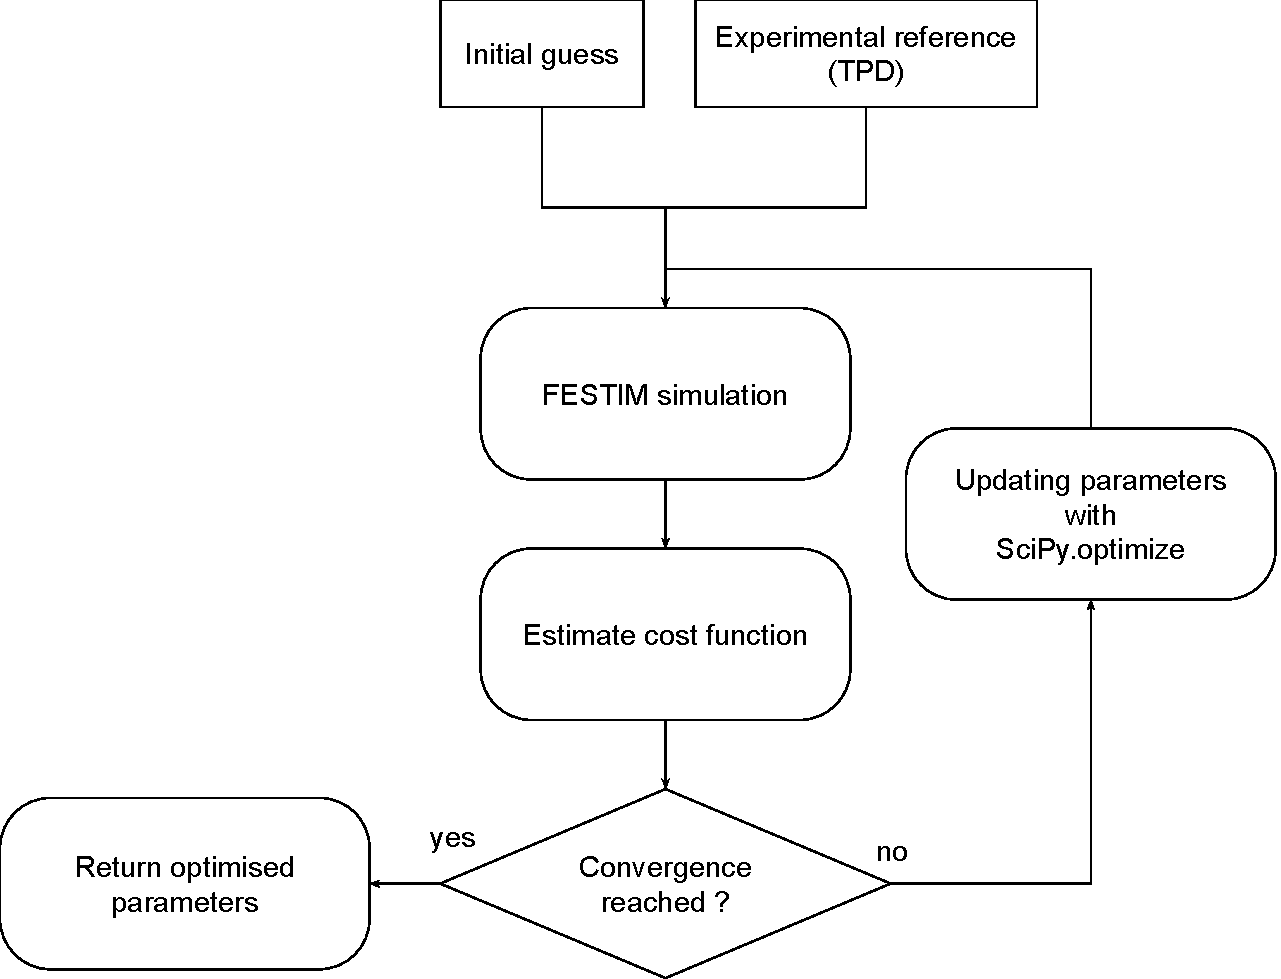
\includegraphics[width=\linewidth]{Figures/Chapter3/Parametric_optimisation/algorithm diagram.pdf}
    \caption{Diagram of the embedding of FESTIM within a parametric optimisation routine based on SciPy \cite{virtanen_scipy_2020}}
    \label{fig:diagramm}
\end{figure}

A comparative study of the several optimisation algorithms which can be employed is made in Section \ref{optimisation algorithms}.
These algorithms require the user to give an initial set of parameters called \textit{initial guess} and evaluate the cost function with several parameters sets until the convergence criterion is reached.
As in \sidecite{drexler_model-based_2019}, the Python package SciPy \sidecite{virtanen_scipy_2020} will be employed.

\subsection{Optimisation algorithms} \label{optimisation algorithms}
In this Section, four minimisation algorithms are benchmarked against a test case.
In the following example an experimental TPD spectrum from Ogorodnikova \textit{et al.} \sidecite{ogorodnikova_deuterium_2003} will be fitted and materials properties such as trap density and detrapping energy will be identified.
For this example case, two intrinsic traps and one extrinsic trap are set.
The only free parameters are $E_1$ and $n_1$, respectively the detrapping energy and density of trap 1.
The other parameters are constrained and described in \sidecite{delaporte-mathurin_finite_2019}.
The cost function $f$ has been plotted on Figure \ref{fig:cost function} as function of $E_1$ and $n_1$.

\begin{figure*} [ht]
    \centering
        \begin{subfigure}[t]{0.5\linewidth}
            \centering
            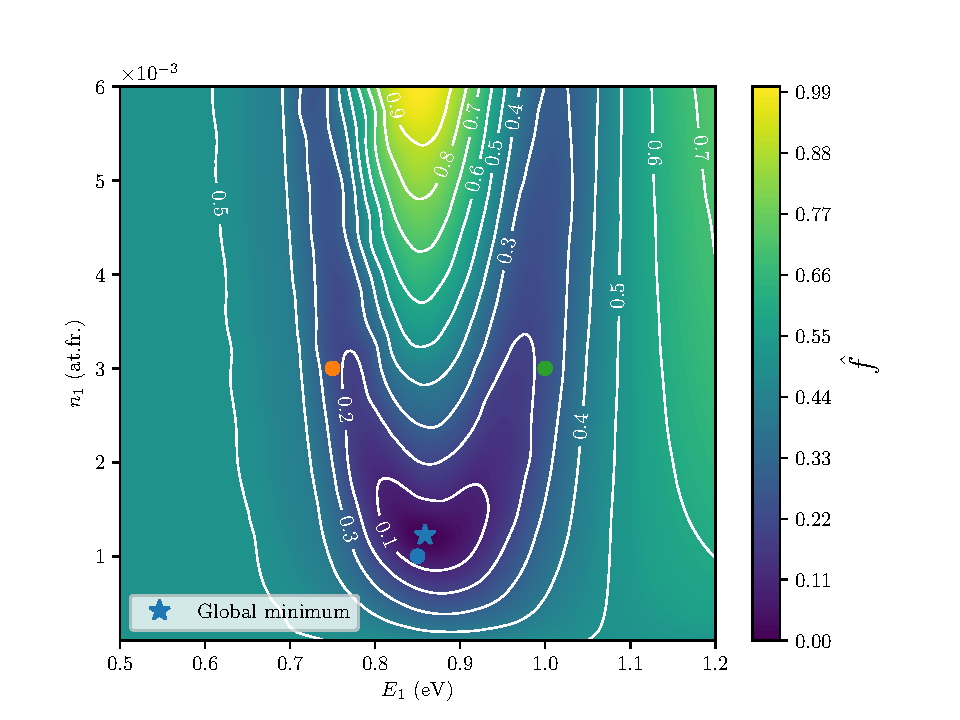
\includegraphics[width=\linewidth]{Figures/Chapter3/Parametric_optimisation/cost_function_2D.pdf}
            \caption{Normalised cost function}
            \label{fig:2D}
        \end{subfigure}%
        \begin{subfigure}[t]{0.5\linewidth}
            \centering
            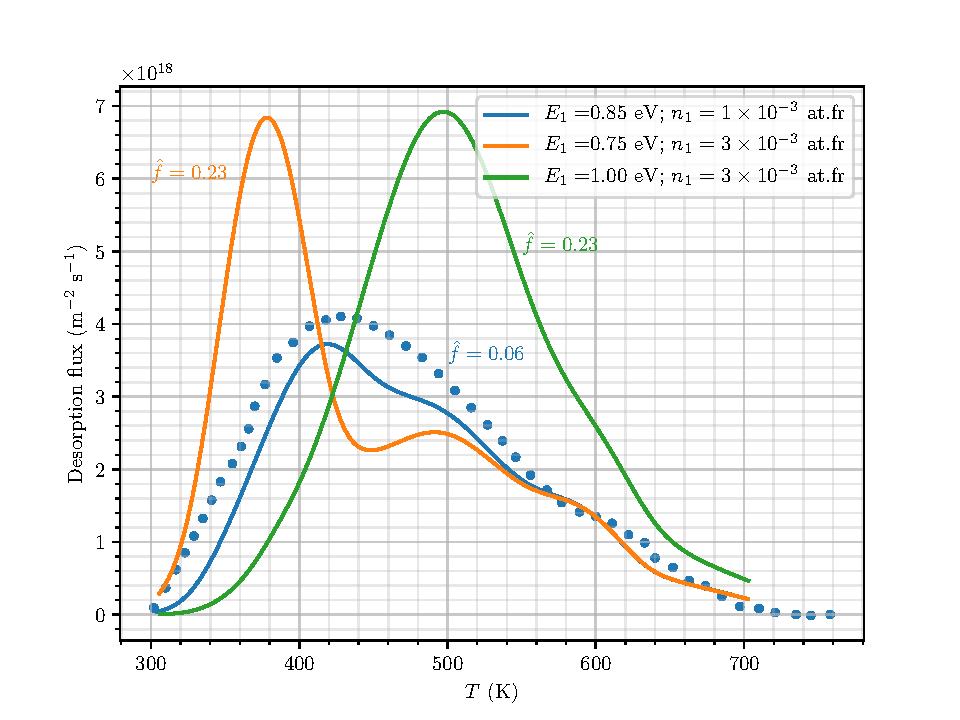
\includegraphics[width=\linewidth]{Figures/Chapter3/Parametric_optimisation/points_on_cost_function.pdf}
            \caption{Corresponding simulated TPD spectra}
            \label{fig:corresponding spectra}
        \end{subfigure}%
    \caption{Normalised cost function $\hat{f} = (f - \min{f})/(\max{f}-\min{f})$ as function of $E_1$ (\si{eV}) and $n_1$ (\si{at.fr.}) with global minimum located at $(\SI{0.86}{eV}, \SI{1.2e-3}{at.fr.})$.}
    \label{fig:cost function}
\end{figure*}

In this case, when only 2 free parameters are set the cost function has only one minimum (it is not necessarily the case for higher dimension optimisation problems).
However, if one fixes the trap density $n_1$ above $\approx \SI{2e-3}{at.fr.}$, the cost function has two local minima which can lead the optimisation routine to converged to a non-global minimum.
Moreover, $f$ is smooth and quadratic around its minimum located at $(E_1, n_1) = (\SI{0.86}{eV}, \SI{1.2e-3}{at.fr.})$.
For detrapping energies below \SI{0.6}{eV} and/or densities below \SI{0.5e-3}{at.fr}, the cost function is constant.
This is because for these values, the contribution of this trapping site to the TPD spectrum is zero either because the density is close to zero, or because the energy is too low for these traps to be filled at the implantation temperature of \SI{300}{K}.
Variations in these regions do not modify the simulated spectrum and thus do not modify the cost function value.

\begin{figure} [ht]
    \centering
    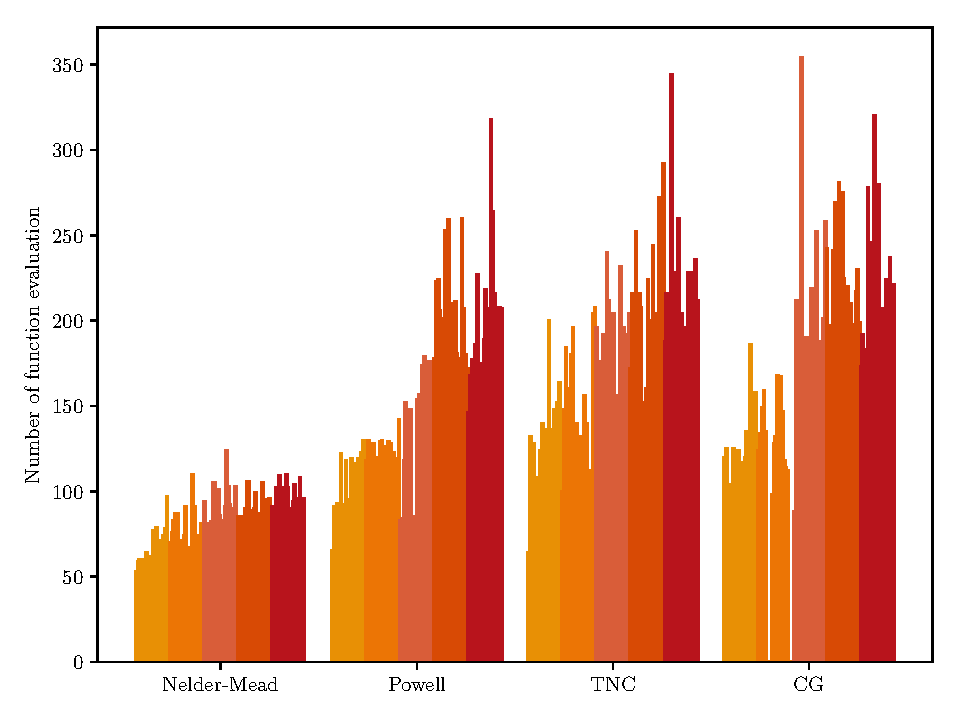
\includegraphics[width=\linewidth]{Figures/Chapter3/Parametric_optimisation/algorithms_perfs.pdf}
    \caption{Number of cost function evaluations required to converge towards the global minimum with 100 different initial guesses sorted by distance to the global minimum for several minimisation algorithms. Each cost function evaluation takes \SI{20}{s} to compute. White stripes correspond to initial guesses for which the algorithm did not converge to the global minimum.}
    \label{fig:algos perfs}
\end{figure}


Four different optimisation algorithms are being compared: 
Nelder-Mead (also called the simplex method), Powell, Truncated Newton method (TNC) and Conjugate Gradient (CG).
Thorough descriptions of these algorithms would be beyond the scope of this study but can be found in \sidecite{nocedal_numerical_2006}.
The performances of these algorithms have been compared with 100 different initial guesses randomly distributed on the $(E_1,n_1)$ plane and are shown on Figure \ref{fig:algos perfs}.
It appears that the CG algorithm is less robust since for some cases it didn't converge towards the global minimum (see white bands on Figure \ref{fig:algos perfs}).
Nelder-Mead algorithm appears to be the most efficient with initial guesses both close and far from the global minimum since the number of cost function evaluations ranges from 50 to 100 whereas other algorithms require more than 100.
This can be explained by the fact that Nelder-Mead is a derivative-free algorithm whereas TNC (Truncated Newton method) and CG algorithms need on the other hand to compute first order derivatives thus increasing the number of function evaluations.
This will be even more true when increasing the number of free parameters since the derivative will become more costly to compute.

It is worth noting that the Nelder-Mead algorithm is an unconstrained method.
If constraints or bounds are needed, TNC might be a more suitable choice.

Though in the following, the Nelder-Mead algorithm will be employed.


\subsection{Results} \label{results}

% \subsection{Applications}

The fitting procedure has been employed to reproduce thermo-desorption experiments performed on Tungsten, EUROFER, Aluminium and Beryllium.


\subsubsection{Tungsten}

The TPD spectrum measured by Ogorodnikova \textit{et al} presented in Section \ref{optimisation algorithms} has been reproduced by setting all traps parameters as free parameters.
The fitting procedure has been run for several numbers of traps as shown on Figure \ref{fig:number of traps comparison}.
It is clear that setting only one trap is not sufficient to reproduce the experimental data.
The two traps case shows better results but also has a discrepancy near \SI{600}{K}.
This discrepancy is removed when setting a third extrinsic trap to the simulation.

For this last case, the five free parameters are the detrapping energies $E_{p, 1}$, $E_{p, 2}$, $E_{p, 3}$ and densities $n_1$, $n_2$ (the third trapping site being created during the implantation, for which the creation parameters are not part of the free parameters and taken from \sidecite{ogorodnikova_deuterium_2003} or \sidecite{hodille_macroscopic_2015}).
This optimisation case is therefore a 5D optimisation problem.
Every other parameters are taken from \sidecite{hodille_macroscopic_2015}.
The resulting fit is shown on Figure \ref{fig:5D TPD} alongside with the contribution of each trap to the total spectrum.
% (1 trap [ 0.88368005  1.44347635] 2 traps [ 0.83582125  1.23768655  0.98708714  6.85457283])
\begin{figure*} [ht]
    \centering
        \begin{subfigure}[t]{0.5\linewidth}
            \centering
            \captionsetup{width=.9\linewidth}
            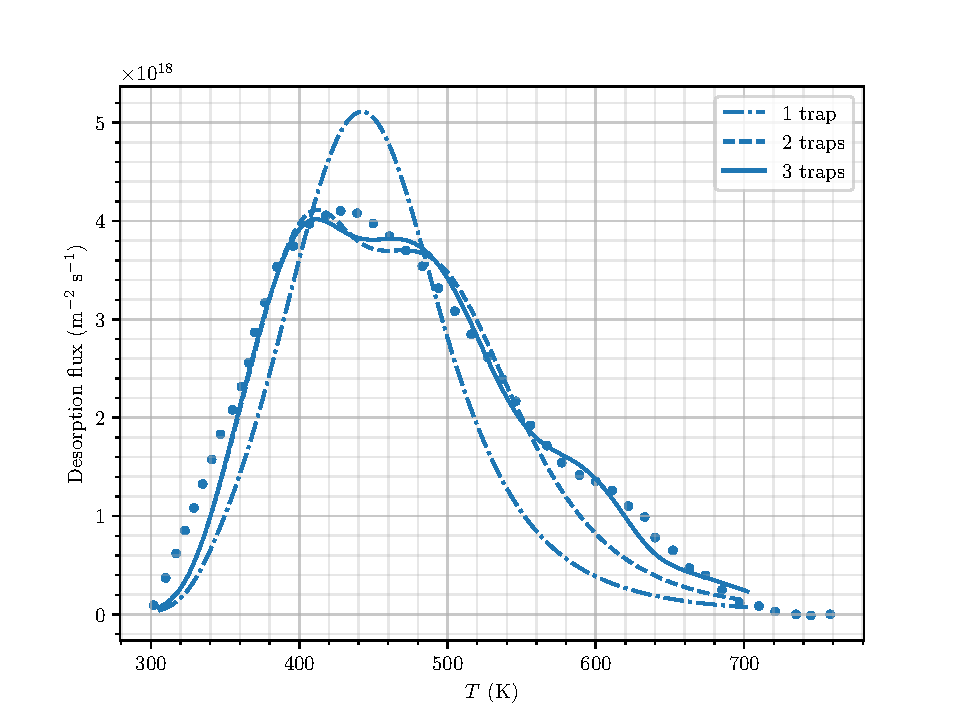
\includegraphics[width=\linewidth]{Figures/Chapter3/Parametric_optimisation/number_of_traps.pdf}
            \caption{Comparison of the resulting fit with several numbers of traps in the simulation.}
            \label{fig:number of traps comparison}
        \end{subfigure}%
        \begin{subfigure}[t]{0.5\linewidth}
            \centering
            \captionsetup{width=.9\linewidth}
            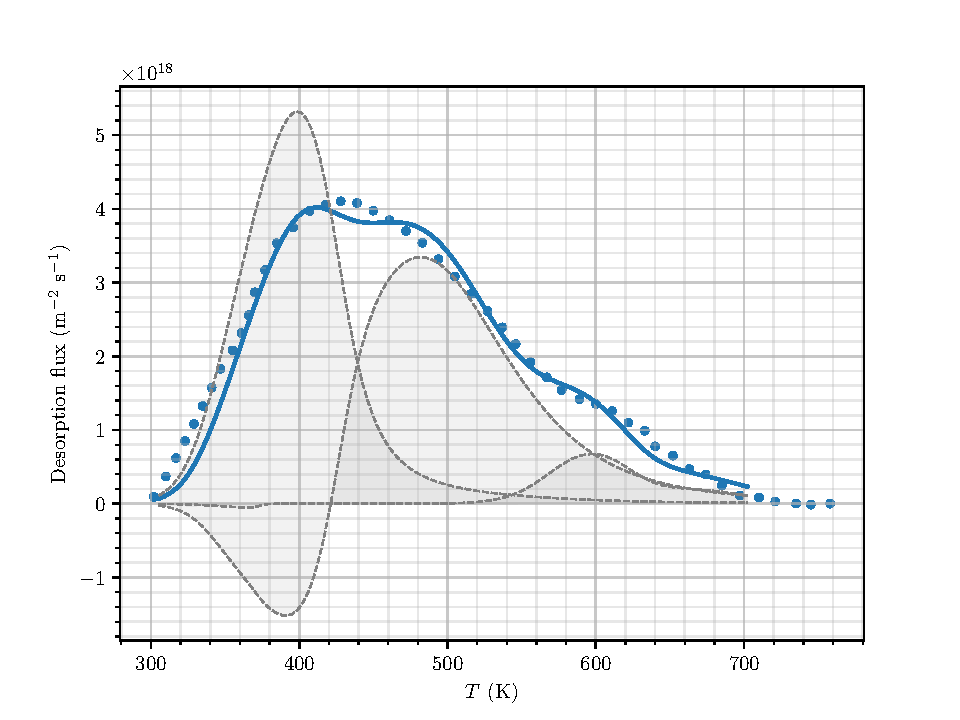
\includegraphics[width=\linewidth]{Figures/Chapter3/Parametric_optimisation/Ogorodnikova_5D.pdf}
            \caption{Identified by the fitting procedure with $E_1 = \SI{0.83}{eV}$, $E_2 = \SI{0.97}{eV}$, $E_3 = \SI{1.51}{eV}$, $n_1 = \SI{1.18e-3}{at.fr.}$ and \newline $n_2 = \SI{7.22e-4}{at.fr.}$.  Dashed lines correspond to the temporal evolution of each trapping population's inventory.}
            \label{fig:5D TPD}
        \end{subfigure}%
    \caption{Fitting TPD spectrum performed on Tungsten by Ogorodnikova \textit{et  al} \cite{ogorodnikova_deuterium_2003}. Dots correspond to experimental data.}
    \label{fig:TPD ogorodnikova}
\end{figure*}
The identified parameters are similar to the ones found by Hodille \textit{et al.} in \sidecite{hodille_macroscopic_2015}.
The total fitting procedure took a few hundred of cost function evaluations.
One single cost function evaluation "costing" less than \SI{20}{s} to compute (for that specific case), the total procedure lasted less than \SI{3}{h}.

\subsubsection{EUROFER}

Hollingsworth \textit{et al} performed thermo-desorption on pre-damaged EUROFER at several damage levels \sidecite{hollingsworth_comparative_2019}.
Three spectra with similar exposure conditions have been fitted with one trapping site (since only one peak appears on the spectra) as shown on Figure \ref{fig:TPD EUROFER}.

\begin{figure} [ht]
    \centering
    \includegraphics[width=\linewidth]{Figures/Chapter3/Parametric_optimisation/EUROFER_hollingsworth.pdf}
    \caption{TPD spectra of damaged EUROFER \cite{hollingsworth_comparative_2019}. Fitted with one trapping site (solid line) $E=\SI{1.06}{eV}$ and densities of \SI{8.9e-3}{at.fr}, \SI{2.8e-2}{at.fr} and \SI{5.0e-2}{at.fr} for \SI{0}{dpa}, \SI{0.01}{dpa} and \SI{0.1}{dpa}, respectively. Dashed lines correspond to optimisations with an unweighted cost function. Dots correspond to experimental data.}
    \label{fig:TPD EUROFER}
\end{figure}

To put the emphasis on peaks, a weighting factor of 10 has been applied for $T \in [\SI{445}{K}, \SI{492}{K}]$.
Not applying this factor near the peak region results in a closer fit in other regions but a higher peak value.
The identified trap energy is $E_p$ \SI{1.06}{eV} for all spectra whereas the trap density $n$ is \SI{8.9e-3}{at.fr} for the undamaged sample, \SI{2.8e-2}{at.fr} for \SI{0.01}{dpa} and \newline \SI{5.0e-2}{at.fr} for \SI{0.1}{dpa}.
For all simulations the attempt frequency $p_0$ is \SI{1e13}{s^{-1}} and the diffusion coefficient is taken from \sidecite{esteban_hydrogen_2007}.

The total fitting procedure took less than two hours for fitting the three spectra.
A more thorough study of these experiments could involve constraining the algorithm with profilometry data obtained by Hollingsworth \textit{et al} \sidecite{hollingsworth_comparative_2019}.
Indeed, having a non-homogeneous trapping site distribution could help having a better fit of both the profilometry data and the TPD spectra. 

\subsubsection{Aluminium}

The experiment performed on Aluminium by Quiros \textit{et al} \sidecite{quiros_blistering_2019, quiros_blister_2017} has also been reproduced with FESTIM.

Only one trap has been set in the simulation and its energy $E_p$ and density $n$ are set as free parameters.
Every other parameters are fixed and taken from \sidecite{quiros_blister_2017, quiros_blistering_2019}.
The resulting simulated TPD spectrum is shown on Figure \ref{fig:TPD alu}.
\begin{figure} [ht]
    \centering
    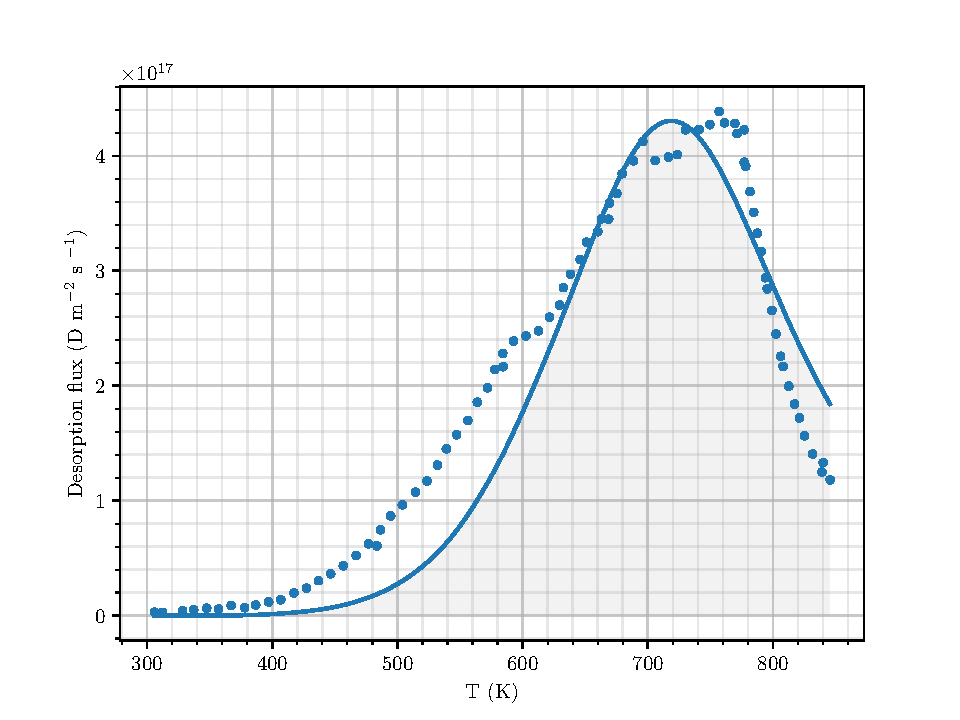
\includegraphics[width=\linewidth]{Figures/Chapter3/Parametric_optimisation/alu_quiros.pdf}
    \caption{TPD spectrum of aluminium exposed to \SI{3e23}{H.m^{-2}} at \SI{618}{K} \cite{quiros_blister_2017, quiros_blistering_2019}. Fitted with one trapping site $n = \SI{1.8e-2}{at.fr.}$ and $E =\SI{1.1}{eV}$. Dots correspond to experimental data. Dashed lines correspond to the temporal evolution of each trapping population's inventory.}
    \label{fig:TPD alu}
\end{figure}


The identified parameters are $n = \SI{1.8e-2}{at.fr.}$ and $E =\SI{1.1}{eV}$.
The trapping sites density is significantly higher than the one described in \sidecite{quiros_blister_2017}.
However, the TPD spectrum obtained with this procedure better fits the experimental data since the one obtained by Quiros \textit{et al} requires a 10-fold increase.
The fitting procedure took less than a hundred cost function evaluations, which corresponds in total to a few dozens of minutes.

\subsubsection{Beryllium}
Be co-deposition experiments performed by Baldwin \textit{et al} \sidecite{baldwin_experimental_2014} were reproduced with FESTIM using this optimisation technique.
In this experiment, a \SI{1}{\micro m} thick Be-D layer is grown on Tungsten at \SI{330}{K}. 
Following the strategy proposed by Baldwin \textit{et al}, only the thermo-desorption phase has been simulated with two trapping sites with homogeneously distributed densities and with initial occupancies $f_i$.
There are therefore three free parameters per trap (energy, density and initial occupancy) which makes this optimisation problem 6D.
It is assumed that the surface flux is the net balance between incoming flux from the chamber (very low since the pressure is $\SI{1}{\micro Pa}$) and the molecular recombination flux.
All the other parameters are described in \sidecite{baldwin_experimental_2014}.

The resulting optimised TPD spectrum is shown on Figure \ref{fig:tpd baldwin}.
The optimised parameters are $E_{p, 1} = \SI{0.75}{eV}$, $n_1 = \SI{1.09e-1}{at.fr.}$, $f_1=0.73$, $E_{p, 2} = \SI{0.93}{eV}$, \newline ${n_2 = \SI{3.40e-2}{at.fr.}}$, $f_2=0.28$.
These values are in agreement with the ones found by Baldwin \textit{et al} \sidecite{baldwin_experimental_2014} and took only a few of minutes to compute since the implantation phase was not simulated.

\begin{figure}
    \centering
    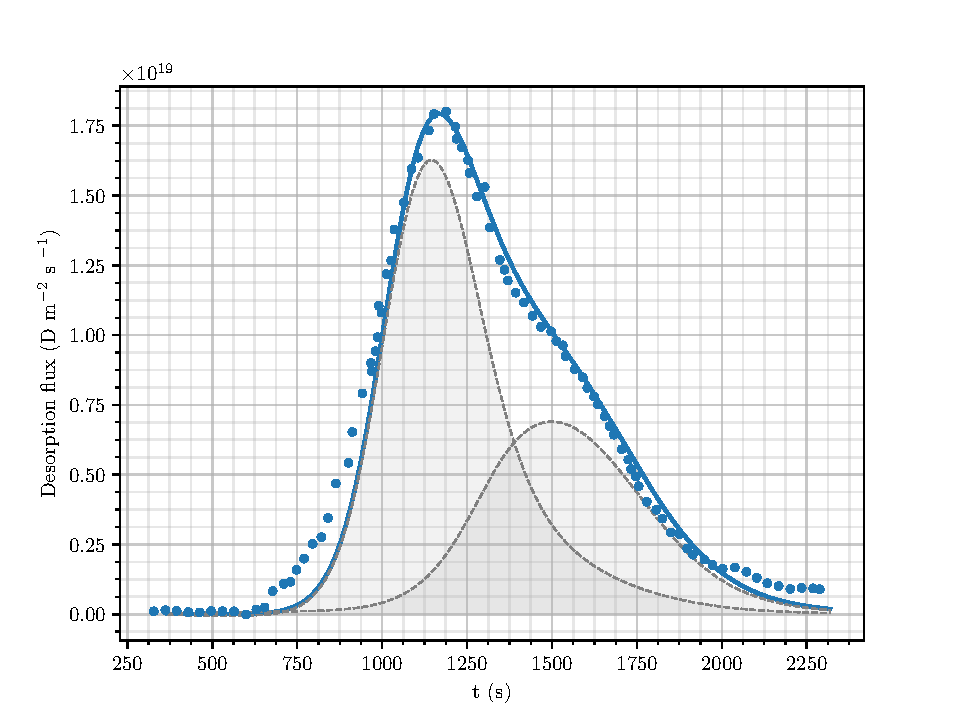
\includegraphics[width=\linewidth]{Figures/Chapter3/Parametric_optimisation/baldwin_be.pdf}
    \caption{TPD spectrum of co-deposited Be-D \cite{baldwin_experimental_2014} simulated with two trapping sites. Dots correspond to experimental data.}
    \label{fig:tpd baldwin}
\end{figure}

\subsection{Discussion}

Even though an automated technique is proposed, the user still has some choices to make in order to ensure the credibility of the fitted spectrum.
As shown on Figure \ref{fig:TPD EUROFER}, weighting the cost function near regions of interest will result in a better fit in these regions.
Users should also be aware of the number of traps the data is being fitted with.
As shown on Figure \ref{fig:number of traps comparison} too few traps in the simulation will not result in a satisfactory fit (even though the optimisation routine will converge to an optimised solution).
Moreover, as shown on Figure \ref{fig:hurley_comparison}, one single TPD spectrum can be reproduced with several traps of different energies and densities.
This means that the cost function with several traps as free parameters can have several local minima of very similar values.
Adding traps to an optimisation problem can also help having a better fit of the experimental data in some cases.
But artificially adding more and more traps is not necessarily realistic and could lead to misinterpretation of the results.

\begin{figure}[ht]
    \centering
    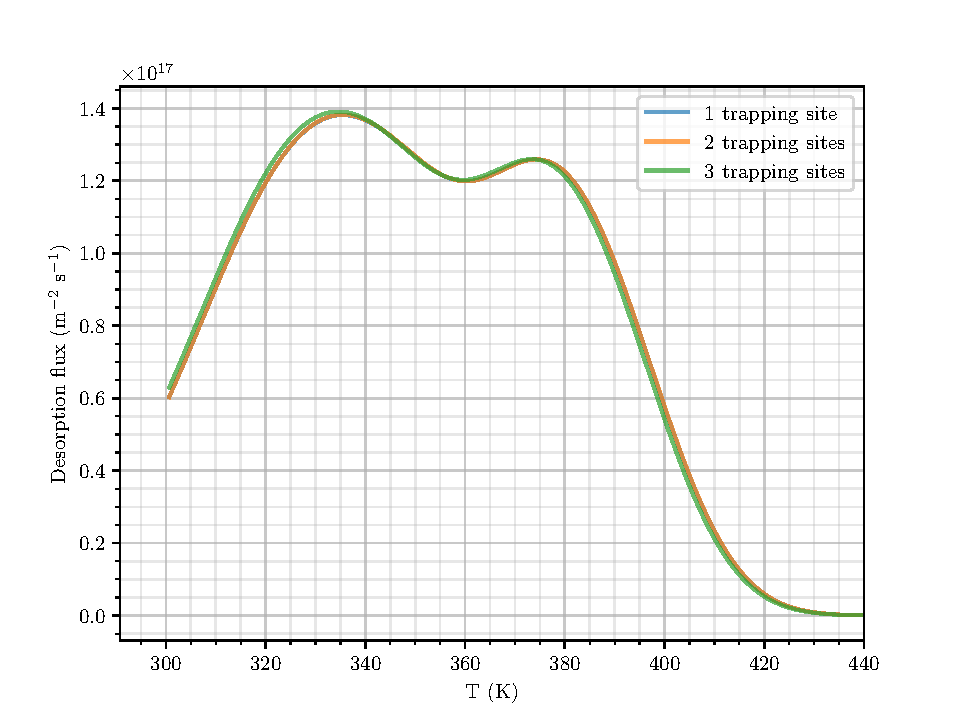
\includegraphics[width=\linewidth]{Figures/Chapter3/Parametric_optimisation/hurley_comparison.pdf}
    \caption{TPD spectrum reproduced with several sets of parameters showing the existence of several solutions to a single optimisation problem.}
    \label{fig:hurley_comparison}
\end{figure}

In the first case with only one trapping site, as described by Hurley \textit{et al} in \sidecite{hurley_numerical_2015}, the binding energy is \SI{0.55}{eV} and the trap density is \SI{2.08e24}{m^{-3}}.
The appearance of two peaks is due to the desorption on different sides of the sample as explained in \sidecite{hurley_numerical_2015}.
In the second case, the curve as been reproduced with two trapping sites which energies and densities are respectively \SI{0.51}{eV} and \SI{0.57}{eV} and \SI{2.02e24}{m^{-3}} and \SI{2.12e24}{m^{-3}}.
In the third case, it has been reproduced with three trapping sites which energies and densities are respectively \SI{0.55}{eV}, \SI{0.38}{eV} and \SI{0.51}{eV} and \SI{2.12e24}{m^{-3}}, \SI{2.26e24}{m^{-3}} and \newline \SI{2.13e24}{m^{-3}}.

This example illustrates how a single spectrum can be simulated with several sets of parameters by varying the number of traps in the simulation.
One way to avoid this from happening is to have a set of experiments with varying parameters such as the implantation temperature, the heating ramp, the fluence, dwelling time before TPD, etc.


\subsection{Summary}
A novel technique for hydrogen transport properties has been demonstrated based on TPD experiments.
By embedding FESTIM in a parametric optimisation routine, one can rapidly (from a few dozens of minutes to a few hours for complex cases) reproduce experimental data and therefore identify parameters such as trapping sites binding energies and densities.

The performances of several optimisation algorithms have been studied and the Nelder-Mead algorithm seems to be the most efficient.
This hydrogen transport properties identification technique has been applied to Tungsten, Aluminium, EUROFER and Beryllium with successful outcome.
Moreover, this technique provides a tool for experimenters to rapidly analyse their data and extract information with ease.
Limitations of this technique such as the choice of the number of trapping sites or the existence of several local minima have been shown.
Including other experiments that would provide profilometry data (such as NRA or SIMS) in order to constrain the optimisation algorithm is a way of improving the accuracy of the results.

This tool could be employed in the future to reproduce permeation experiments or identify surface properties such as recombination coefficients or solubilities.


\section{Divertor}
\subsection{Monoblocks}
\subsubsection{Influence of interface conditions}
\subsubsection{Influence of cycling}
\subsubsection{Parametric study}

% \subsection{Simulation description}
The first step of the work was to simulate the hydrogenic transport and trapping in a tungsten monoblock as a function of the loading conditions.

Moreover, a parametric study will be carried out in order to simulate the whole range of the implantation conditions encountered in the ITER divertor.

% \subsubsection{Geometry}
The geometry used in this work is that of a non-shaped ITER monoblock (see Figure \ref{fig:monoblock geometry}).
The monoblocks use tungsten armour and a \SI{1.5}{mm}-thick CuCrZr pipe as heat sink.
The pipe is jointed to the tungsten.
A \SI{1}{mm}-thick Cu interlayer is used in order to handle stress resulting from differential thermal expansion \cite{richou_realization_2017}.
The surface $\Gamma_\mathrm{top}$ is facing the plasma and $\Gamma_\mathrm{coolant}$ is cooled by water.

\begin{figure} [ht!]
    \centering
    \begin{overpic}[width=0.5\linewidth]{Figures/Chapter3/monoblocks/parametric_study/monoblock_sketch.pdf}
        \put(42, 5){\SI{28}{mm}}
        \put(97, 50){\SI{28}{mm}}
        \put(10, 32){\SI{13.5}{mm}}
        \put(42, 62){ \diameter \SI{12}{mm}}
        \put(42, 71){ \diameter \SI{15}{mm}}
        \put(42, 78){ \diameter \SI{17}{mm}}
        \put(20, 80){\large$\Gamma_\mathrm{top}$}
        \put(40, 41){\large$\Gamma_\mathrm{coolant}$}
    \end{overpic}
    \caption{Monoblock geometry showing W armour \cruleme[grey]{0.3cm}{0.3cm}, Cu interlayer \cruleme[orange]{0.3cm}{0.3cm}, CuCrZr alloy cooling pipe  \cruleme[yellow]{0.3cm}{0.3cm}}
    \label{fig:monoblock geometry}
\end{figure}

% \subsubsection{Material properties}
The material properties used in these simulations are described in Tables \ref{tab:materials properties} and their temperature dependence is shown in Figure \ref{fig:properties}.
The trap parameters are described in Table \ref{tab:traps monoblock}.
Influence of mechanical fields such as thermal expansion on trap creation \cite{benannoune_multidimensional_2020} was not taken into account in this work.
Hodille \textit{et al} described an extrinsic trap in tungsten created by ion implantation \cite{hodille_macroscopic_2015}.
This trap is assumed to have only a small influence on the macroscopic behaviour of the monoblock and is therefore not taken into account in this work for the sake of simplicity.

\begin{table*}[ht]
    \centering
    \begin{tabular}{p{1.7cm}  R{3cm}  R{3cm}  R{1.8cm}  R{2.1cm} }
         & \multicolumn{2}{c}{Thermal properties} & \multicolumn{2}{c}{Hydrogen transport}\\
        \hline
        Material & $\rho \cdot C_p \newline(\si{J.K^{-1}.m^{-3}})$ & $\lambda \newline(\si{W.m^{-1}.K^{-1}})$ & $D_0 \newline(\si{m^2.s^{-1}})$ & $E_\mathrm{diff} \newline(\si{eV})$\\
        \hline
        \\
        W & %
        $5.1\times 10^{-6} \cdot T^3 \newline - 8.3\times 10^{-2}\cdot T^2 \newline + 6.0 \times 10^{2}\cdot T \newline +2.4\times 10^6$ &%
        $-7.8\times 10^{-9}\cdot T^3 \newline %
        +5.0\times 10^{-5}\cdot T^2 \newline%
        -1.1\times 10^{-1} \cdot T \newline%
        +1.8\times 10^{2}$ &%
        $1.9\times 10^{-7}$ & 0.20 \\
        \\
        Cu &%
        $1.7\times 10^{-4}\cdot T^3\newline %
        +6.1\times 10^{-2}\cdot T^2\newline %
        +4.7\times 10^2\cdot T\newline %
        +3.5\times 10^6$ &%

        $-3.9\times 10^{-8}\cdot T^3\newline %
        +3.8\times 10^{-5}\cdot T^2\newline %
        -7.9\times 10^{-2}\cdot T\newline %
        +4.0\times 10^2 $&%

        $6.6\times 10^{-7}$ &%
        0.39\\
        \\
        CuCrZr & %
        $-1.8\times 10^{-4}\cdot T^3 \newline %
        +1.5\times 10^{-1}\cdot T^2\newline %
        +6.2\times 10^2\cdot T\newline %
        +3.5\times 10^6$ &%

        $5.3\times 10^{-7}\cdot T^3\newline %
        -6.5\times 10^{-4}\cdot T^2\newline %
        +2.6\times 10^{-1}\cdot T\newline %
        +3.1\times 10^2$ & %

        $3.9\times 10^{-7}$ & %
        0.42\\
        \\
    \end{tabular}
    \caption{Materials properties used in the simulations. Thermal properties are fitted from ANSYS. \cite{reiter_compilation_1996, serra_hydrogen_1998, fernandez_hydrogen_2015}}
    \label{tab:materials properties}
\end{table*}

\begin{figure} [h!]
    \centering
    \begin{subfigure}{0.5\linewidth}
        \centering
        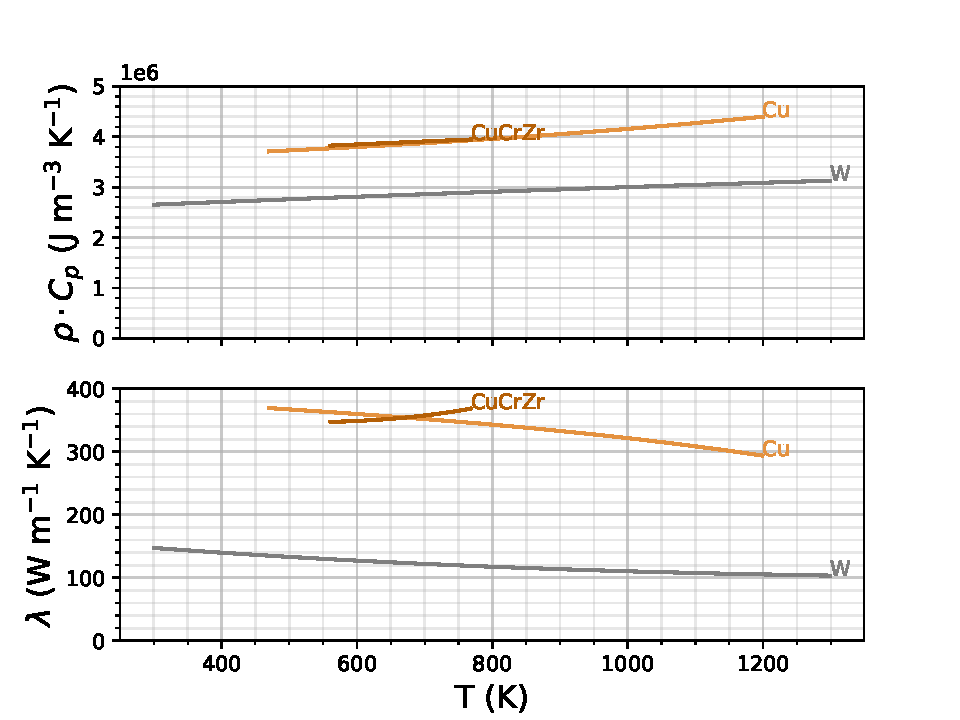
\includegraphics[width=\linewidth]{Figures/Chapter3/monoblocks/parametric_study/thermal_prop.pdf}
        \label{fig:thermal prop}
    \end{subfigure}%
    \begin{subfigure}{0.5\linewidth}
        \centering
        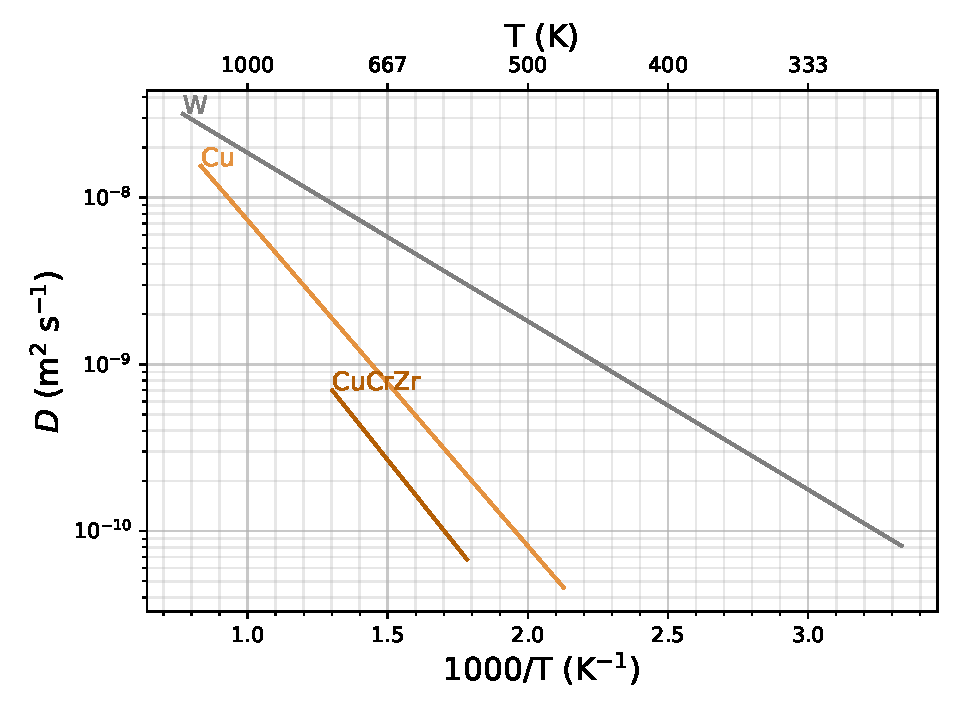
\includegraphics[width=\linewidth]{Figures/Chapter3/monoblocks/parametric_study/D_coeff.pdf}
        \label{fig:D coeff}
    \end{subfigure}
    \caption{Material properties used in the simulations \cite{reiter_compilation_1996, serra_hydrogen_1998, fernandez_hydrogen_2015}}
    \label{fig:properties}
\end{figure}

\begin{table*} [ht]
    \centering
    \begin{tabular}{L{1.5cm} L{1.5cm} R{1.6cm} R{1.1cm} R{1.6cm} R{1.1cm} R{2cm}}
         & Material & $k_0 (\si{m^3.s^{-1}})$ &  $E_k (\si{eV})$ & $p_0 (\si{s^{-1}})$ & $E_p (\si{eV})$ & $n_i (\si{at.fr.})$ \\
        \hline
        \\
       Trap 1 & W & $3.1 \times 10^{-16}$ & 0.20 & $8.4 \times 10^{12}$& 1.00 & $1.1 \times 10^{-3}$ \\
        \\
        Trap 2 & Cu & $6.0 \times 10^{-17}$ & \textcolor{black}{0.39} & $8.0 \times 10^{13}$ & 0.50 &$5.0 \times 10^{-5}$\\
        \\
        Trap 3 & CuCrZr & $1.2 \times 10^{-16}$ & \textcolor{black}{0.42} & $8.0 \times 10^{13}$ & 0.85 &$5.0 \times 10^{-5}$\\
        \\
    \end{tabular}
    \caption{Traps properties used in the simulations \cite{hodille_macroscopic_2015, dolan_assessment_1994}}
    \label{tab:traps monoblock}
\end{table*}

% \subsubsection{Boundary conditions}

Mobile particles concentration $c_\mathrm{m}$ is imposed on $\Gamma_\mathrm{top}$ which allows to simulate particle implantation without having to include a volumetric source term applied on the first few nanometres.
This approximation allows to have a broader mesh and therefore saves computation time without affecting the macroscopic behaviour.
Molecular recombination is assumed on $\Gamma_\mathrm{coolant}$.
Even though it could be assumed on the gaps between monoblocks, it can be shown that its influence on the macroscopic behaviour remains low.
Desorption from the other surfaces is therefore assumed to be zero for simplification purposes.
\textcolor{black}{Uniform} heat loads $\varphi_H$ are applied on the surface $\Gamma_\mathrm{top}$ with a Neumman boundary condition or temperature is constrained on $\Gamma_\mathrm{top}$ with a Dirichlet boundary condition and a convective exchange condition is set on surface $\Gamma_\mathrm{coolant}$.
All the other surfaces are assumed thermally insulated.
The set of boundary conditions can finally be described as follow:

\begin{eqnarray}
    -\lambda \vec{\nabla} T \cdot \vec{n} &=\varphi_{H} \quad \text{or} \quad T = T_\mathrm{surface}\quad &\text { on } \Gamma_\mathrm{top}\\
    \qquad \quad c_\mathrm{m} &=  c_\mathrm{surface}\quad &\text { on } \Gamma_\mathrm{top}\\
    -\lambda \vec{\nabla} T\cdot \vec{n} &= -h \cdot \left(T_\mathrm{coolant} - T\right)\quad &\text { on } \Gamma_\mathrm{coolant}\\
    -D \vec{\nabla} c_\mathrm{m} \cdot \vec{n} &= K_\mathrm{CuCrZr} \cdot c_\mathrm{m}^{2} \quad &\text { on } \Gamma_\mathrm{coolant}
\end{eqnarray}
with $h=\SI{70000}{W.m^{-2}.K^{-1}}$ being the heat exchange coefficient calculated from the Sieder-Tate correlation for the forced convection regime, $T_\mathrm{coolant}= \SI{323}{K}$ and $\vec{n}$ the normal vector and $K_\mathrm{CuCrZr} = 2.9 \times 10^{-14}\cdot \exp{(-1.92/(k_B\cdot T))}$ the recombination coefficient of the copper alloy (in vacuum) expressed in \si{m^4.s^{-1}} \cite{anderl_deuterium_1999}.

% The thermal response of ITER-like monoblocks to the heat load $\varphi_H$ has first been studied.
% Then the hydrogen inventory was determined as a function of surface temperature and surface concentration and as a function of the implanted particle flux and the incident ion energy.
% Finally, an application on ITER exposure conditions was made.

\subsection{Thermal behaviour}
Steady-state heat transfer simulations were performed with FESTIM with varying heat loads $\varphi_H$.
With $\varphi_H = \SI{1}{MW.m^{-2}}$, the surface temperature of the monoblock was found to be around \SI{400}{K} (see Figure \ref{fig:T field 1 MW}) whereas with $\varphi_H = \SI{10}{MW.m^{-2}}$ the surface was around \SI{1400}{K} (see Figure \ref{fig:T field 10 MW}).

\begin{figure*} [h!]
    \centering
    \begin{subfigure}{0.4\linewidth}
        \centering
        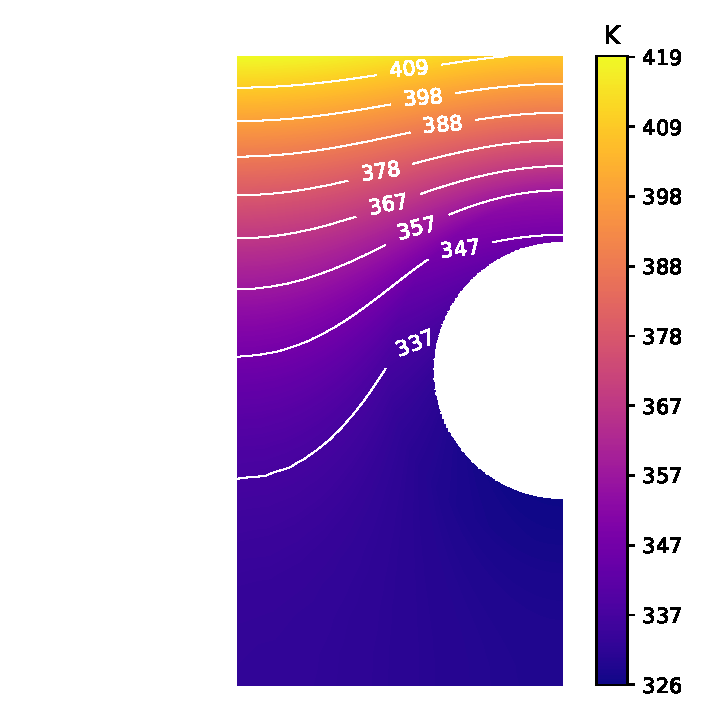
\includegraphics[width=\linewidth]{Figures/Chapter3/monoblocks/parametric_study/T_1e6.pdf}
        \caption{Temperature field with $\varphi_H = \SI{1}{MW.m^{-2}}$}
        \label{fig:T field 1 MW}
    \end{subfigure}%
    \begin{subfigure}{0.4\linewidth}
        \centering
        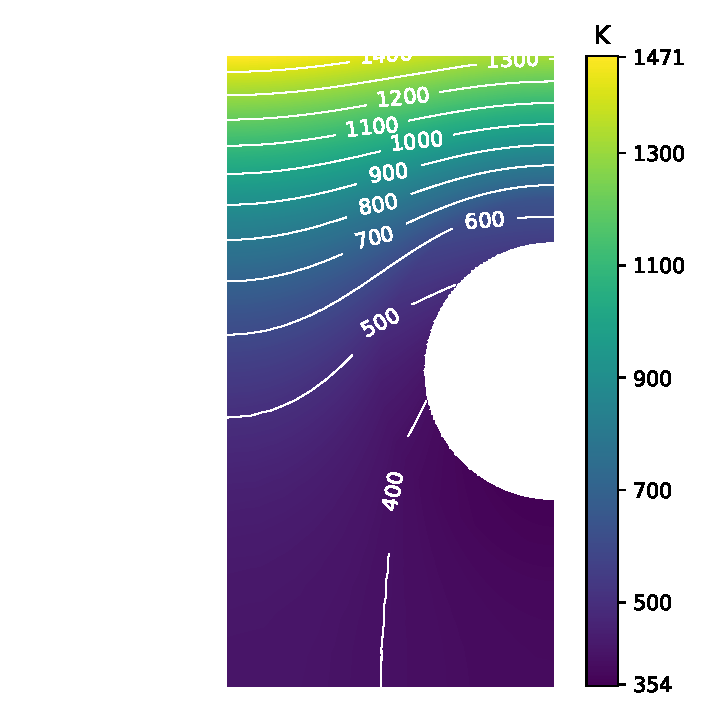
\includegraphics[width=\linewidth]{Figures/Chapter3/monoblocks/parametric_study/T_1e7.pdf}
        \caption{Temperature field with $\varphi_H = \SI{10}{MW.m^{-2}}$}
        \label{fig:T field 10 MW}
    \end{subfigure}
    \begin{subfigure}{0.7\linewidth}
        \centering
        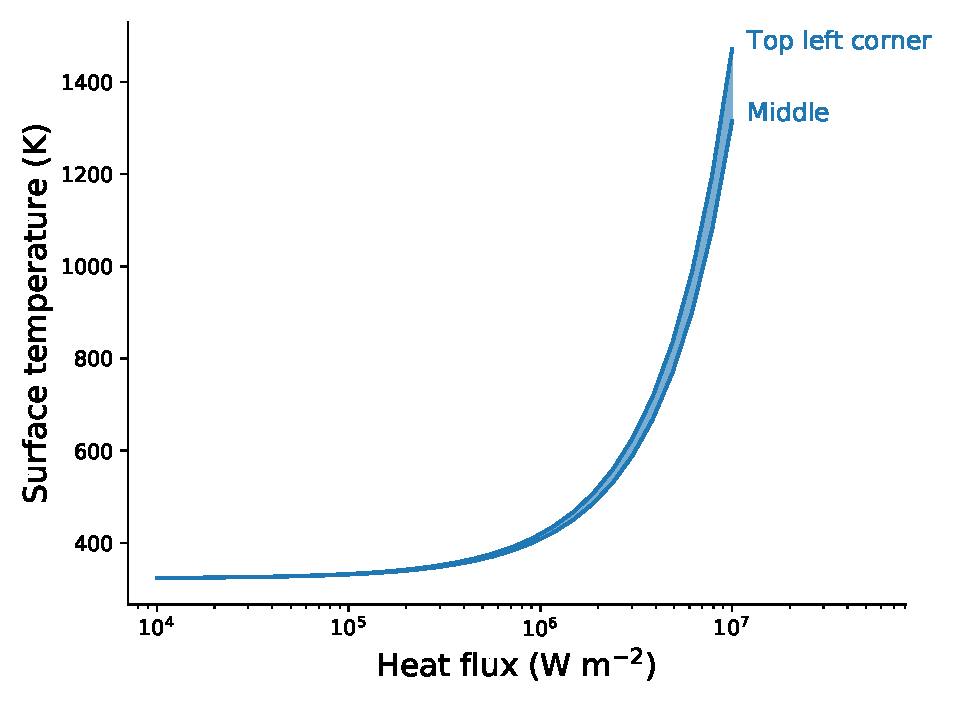
\includegraphics[width=\linewidth]{Figures/Chapter3/monoblocks/parametric_study/temperature_phi_H.pdf}
        \caption{\textcolor{black}{Evolution of surface temperature as a function of heat flux}}
        \label{fig:T phi_H}
    \end{subfigure}
    \caption{Thermal behaviour of the monoblock}
\end{figure*}

\textcolor{black}{
In order to simplify the analytical relations used in Section \ref{particle and energy}, only the mean surface temperature was considered in the following sections.
}
$T_\mathrm{surface}$ \textcolor{black}{therefore} increases linearly with the heat load and can be modelled by Equation \ref{eq:thermal behaviour law} (see Figure \ref{fig:T phi_H}).
\begin{equation}
    T_\mathrm{surface} = 1.1 \times 10^{-4} \cdot \varphi_H + T_\mathrm{coolant}
    \label{eq:thermal behaviour law}
\end{equation}

This was found to be in very good agreement with experimental measurements performed in \cite{hirai_use_2016}.

\subsection{Influence of \texorpdfstring{$T_\mathrm{surface}$}{Tsurface} and \texorpdfstring{$c_\mathrm{surface}$}{csurface} on hydrogen inventory}

In this section, the total inventory of hydrogen in monoblocks has been calculated as a function of $T_\mathrm{surface}$ and $c_\mathrm{surface}$.
Temperature and mobile concentration of hydrogen were imposed with Dirichlet boundary conditions on $\Gamma_\mathrm{top}$ with $T_\mathrm{surface}$ varying from $T_\mathrm{coolant}$ to \SI{1200}{K} and $c_\mathrm{surface}$ varying \textcolor{black}{arbitrarily} from \SI{e20}{m^{-3}} to \SI{6e22}{m^{-3}}.
The assumption of a constant surface temperature had low influence on the results compared to a non-homogeneous surface temperature that could be obtained with a heat flux condition since surface temperature gradient was low compared to the one between the top surface and the cooling surface.
For surface temperatures below \SI{500}{K}, 1D simulations were performed for the penetration depth of hydrogen remained very low (a few microns) and 1D approximation was sufficient \cite{benannoune_numerical_2019}.
For temperatures above \SI{500}{K} for which edge effects become dominant, 2D simulations have been performed.

After $ \SI{e7}{s}$ a high retention zone appeared far from the exposed surface $\Gamma_\mathrm{top}$ (see Figure \ref{fig:retention fields}).
As described in \cite{delaporte-mathurin_finite_2019}, this is due to thermal effects.
As seen in Figures \ref{fig:T field 1 MW} and \ref{fig:T field 10 MW}, the temperature was found to decrease in regions close to the cooling pipe $\Gamma_\mathrm{coolant}$ leading to an increase in trap occupancy, creating this high retention zone.
This was however not true for monoblocks where $T_\mathrm{surface} \approx T_\mathrm{coolant}$ since the temperature gradient in the domain is very low.
Instead, trap occupancy was close to one and the retention was high in the whole region where hydrogen had penetrated and not only far from the top surface.

\begin{figure*}
    \centering
    \begin{subfigure}{0.5\linewidth}
        \centering
        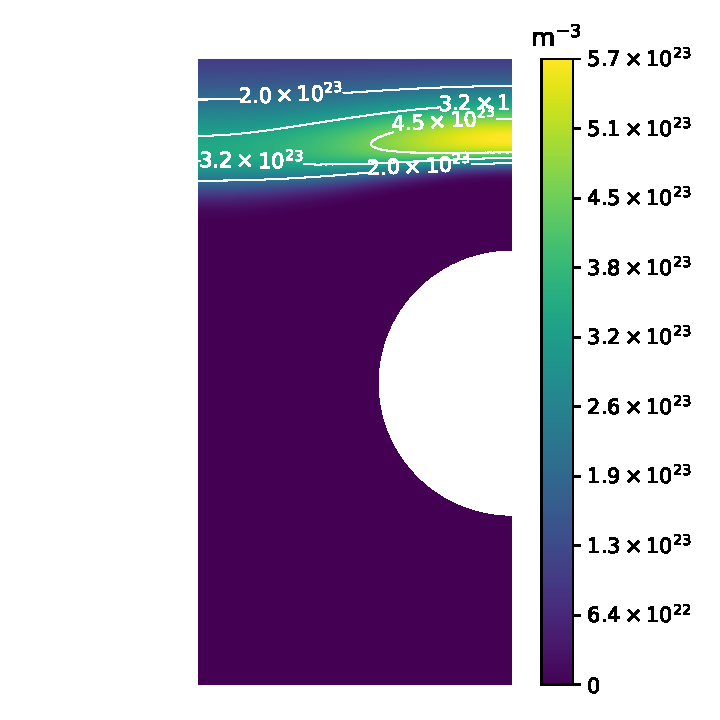
\includegraphics[height=\linewidth]{Figures/Chapter3/monoblocks/parametric_study/retention_T=7.000e+02;c=1.00e+20.pdf}
        \caption{$T_\mathrm{surface} = \SI{700}{K}$ and $c_\mathrm{surface} = \SI{e20}{m^{-3}}$}
    \end{subfigure}%
    \begin{subfigure}{0.5\linewidth}
        \centering
        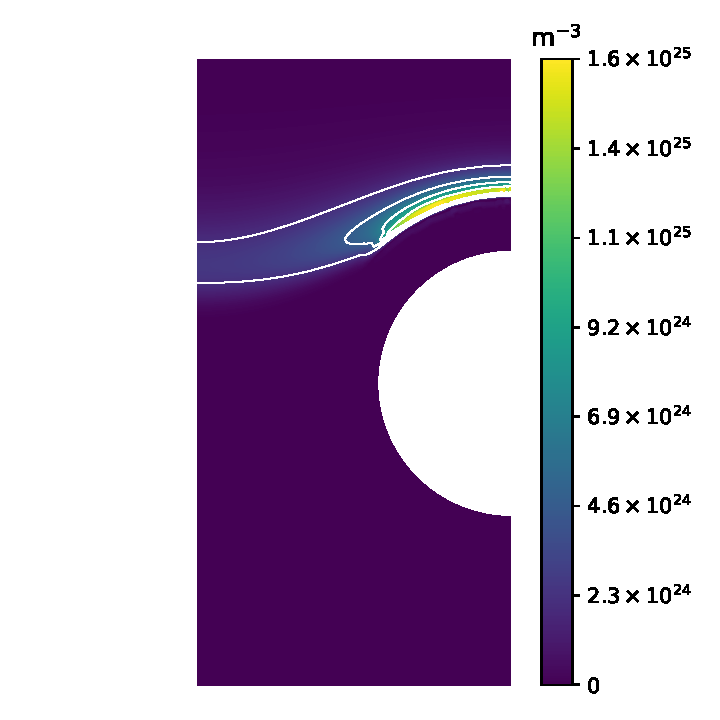
\includegraphics[height=\linewidth]{Figures/Chapter3/monoblocks/parametric_study/retention_T=1.000e+03;c=1.00e+21.pdf}
        \caption{$T_\mathrm{surface} = \SI{1000}{K}$ and $c_\mathrm{surface} = \SI{e21}{m^{-3}}$}
    \end{subfigure}
    \caption{Retention fields in \si{m^{-3}} after a \SI{e7}{s} exposure}
    \label{fig:retention fields}
\end{figure*}


Hydrogen inventory in monoblocks as a function of $T_\mathrm{surface}$ and $c_\mathrm{surface}$ is shown in Figure \ref{fig:inventory T c}.
In order to obtain this continuous field, more than 600 simulations randomly distributed on the parameter plane were run and analysed using a Gaussian process machine learning algorithm \cite{rasmussen_gaussian_2006} as in \cite{shimwell_multiphysics_2019} based on the python package inference-tools \cite{chris_bowman_c-bowmaninference-tools_2020}.
In Figure \ref{fig:inventory T c}, the inventory obtained by the Gaussian regression process is given for a constant value of $c_\mathrm{surf}=\SI{2e21}{m^{-3}}$ (top inset) and a constant temperature $T=\SI{850}{K}$ (left inset).
The Gaussian regression process was particularly appropriate as it calculates a confidence interval based on the standard deviation $\sigma$.
As expected, the lower the density of simulation points, the higher was the value of $\sigma$ (for example around \SI{850}{K} on the top inset of Figure \ref{fig:inventory T c}).
However, despite the lack of simulation in this region, the value of $\sigma$ was still acceptable (only a few percents of the inventory) ensuring the quality of the resulting interpolation.

As expected, inventory was found to globally increase with $c_\mathrm{surface}$.
For $T_\mathrm{surface} > \SI{550}{K}$, the inventory tended to decrease with surface temperature.
However, for $T_\mathrm{surface} < \SI{550}{K}$, inventory increased with surface temperature.
This phenomenon is due to a trade-off between an increase of the detrapping rate and an increase of the diffusion coefficient making the hydrogen particles penetrate deeper into the bulk.
Above $\SI{550}{K}$, detrapping becomes dominant and inventory decreases.
This mapping of inventory as a function of $T_\mathrm{surface}$ and $c_\mathrm{surface}$ provides an easy way of estimating the inventory in monoblocks for several exposure conditions without having to run many simulations.
Indeed, to estimate the inventory with different exposure conditions, one only needs to associate these conditions $(\varphi_\mathrm{inc}, E)$ to a couple $(c_\mathrm{surf}, T_\mathrm{surf})$.

\begin{figure*} [h]
    \centering
    \includegraphics[width=\linewidth]{Figures/Chapter3/monoblocks/parametric_study/inventory_T_c_profiles.pdf}
    \caption{Evolution of the inventory after a \SI{e7}{s} exposure as a function of $T_\mathrm{surface}$ and $c_\mathrm{surface}$ alongside with simulation points (grey crosses). The simulations points were fitted with a Gaussian regression process \cite{chris_bowman_c-bowmaninference-tools_2020} providing the standard deviation $\sigma$.}
    \label{fig:inventory T c}
\end{figure*}

\subsection{Influence of incident particle flux and ion energy on hydrogen inventory} \label{particle and energy}
Incident particle flux $\varphi_\mathrm{inc}$ and ion energy $E$ have an impact on the amount of mobile particles implanted in the material but also on the heat load and therefore on the surface temperature of the monoblock.

Assuming a source term with a narrow Gaussian distribution and a non-instantaneous recombination (characterised by a recombination coefficient $K$), the concentration $c_\mathrm{max}$ at the near surface is approximated by:

\begin{equation}
    c_\mathrm{max} =  \frac{\varphi_\mathrm{imp} \cdot R_p}{D(T_\mathrm{surface})} + \sqrt{\frac{\varphi_\mathrm{imp}}{K(T_\mathrm{surface})}}
    \label{eq:cmax}
\end{equation}

where $\varphi_\mathrm{imp} = (1-r) \cdot \varphi_\mathrm{inc}$ is the implanted particle flux, $r$ is the particle reflection coefficient, $K$ is the recombination coefficient, and $R_p$ is the mean implantation depth in \si{m}.
Details can be found in appendix \textcolor{black}{as Supplementary Material}.
Many different values of the recombination coefficient $K$ for tungsten can be found in literature.
For instance the widely used Anderl coefficient describes an endothermic recombination \cite{anderl_hydrogen_1990} whereas Ogorodnikova showed an exothermic recombination coefficient could be used to reproduce a set of experiments \cite{ogorodnikova_recombination_2019}.

Facing the difficulty of an accurate choice for $K$ and following the recommendation of Causey \textit{et al} \cite{causey_hydrogen_2002}, an instantaneous recombination will therefore be assumed (\textit{ie} $K \rightarrow +\infty$).
It is also worth noting that experiments by Bisson \textit{et al} \cite{bisson_dynamic_2015} support the fact that recombination is not the rate limiting step during the hydrogen release from polycrystalline tungsten after ion implantation.

In the following, the concentration on $\Gamma_\mathrm{top}$ was set to $c_\mathrm{surface} = c_{\mathrm{max}}$ for the kinetics involved are really fast (see appendix of \cite{hodille_hydrogen_2018}) and $R_p$ is small compared to the monoblock dimensions.

The heat load was assumed to evolve as a function of the incident particle flux $\varphi_\mathrm{inc}$ and $E$ as follow:

\begin{equation}
    \varphi_H = 2.2\cdot \varphi_\mathrm{inc} \cdot e \cdot (E + \SI{13.6}{eV})
    \label{eq:phi_H}
\end{equation}
with $e = \SI{1.6e-19}{C}$.
This relation was obtained by fitting SOLPS \textcolor{black}{data \cite{pacher_impurity_2015, khan_walldyn_2019}}.
The factor 2.2 was applied to take into account other heat sources such as radiative flux.

Moreover, the ion energy $E$ has an influence on $r$ and implantation range $R_p$ and it was possible to model the evolution of these parameters with SRIM \cite{ziegler_srim_2010} calculations as follow:
\begin{equation}
    r = 2\times 10^{-8} \cdot E^2 -6 \times 10^{-5} \cdot E + 8\times 10^{-1}
    \label{eq:r}
\end{equation}

\begin{equation}
    R_p = 1.4\times 10 ^{-10}\cdot E^{0.64}
    \label{eq:Rp}
\end{equation}
By combining Equations \ref{eq:phi_H}, \ref{eq:r}, one can obtain the evolution of $\varphi_H$ as a function of $\varphi_\mathrm{inc}$ and $E$ as shown in Figure \ref{fig:phi_H phi E}.
From the thermal behaviour given by Equation \ref{eq:thermal behaviour law}, the surface temperature $T_\mathrm{surface}$ can be computed (see Figure \ref{fig:T_surf phi E}).
Finally, $c_\mathrm{max}$ was obtained from Equations \ref{eq:cmax} and \ref{eq:Rp} (see Figure \ref{fig:c_max_instantaneous}).

\begin{figure*} [ht]
    \centering
    \begin{subfigure}{0.5\linewidth}
        \centering
        \includegraphics[width=\linewidth]{Figures/Chapter3/monoblocks/parametric_study/phi_H_phi_E.pdf}
        \caption{Surface heat flux}
        \label{fig:phi_H phi E}
    \end{subfigure}%
    \begin{subfigure}{0.5\linewidth}
        \centering
        \includegraphics[width=\linewidth]{Figures/Chapter3/monoblocks/parametric_study/T_phi_E.pdf}
        \caption{Surface temperature}
        \label{fig:T_surf phi E}
    \end{subfigure}
    \begin{subfigure}{0.5\linewidth}
        \centering
        \includegraphics[width=\linewidth]{Figures/Chapter3/monoblocks/parametric_study/c_max_instantaneous.pdf}
        \caption{Surface concentration}
        \label{fig:c_max_instantaneous}
    \end{subfigure}%
    \begin{subfigure}{0.5\linewidth}
        \centering
        \includegraphics[width=\linewidth]{Figures/Chapter3/monoblocks/parametric_study/inventory_phi_E.pdf}
        \caption{Monoblock inventory}
        \label{fig:inventory phi E}
    \end{subfigure}
    \caption{$\varphi_H$, $T_\text{surface}$, $c_\mathrm{max}$ and inventory per monoblock as a function of $\varphi_\mathrm{inc}$ and $E$. Inventory has not been calculated for surface temperature above \SI{1200}{K} (greyed region). White circles correspond to points on ITER divertor using the divertor plasma parameters from SOLPS \cite{bonnin_presentation_2016} calculations (see Section \ref{ITER application}).}
    \label{fig:phi_H T_surf c_max}
\end{figure*}

One must be aware that above \SI{1500}{K}, W recrystallisation can occur and H transport will strongly be affected.
The hypothesis made above as well as material properties may then not be valid.
Because of the trade-off between the amount of implanted particles and the resulting heat flux, the maximum value of $c_{\mathrm{max}}$ was found to be \SI{2e22}{m^{-3}} around $(\varphi_\mathrm{inc}, E)=(\SI{8e22}{m^{-2}.s^{-1}}, \SI{20}{eV})$.
Considering the previously calculated response of the monoblock to $c_\mathrm{surface}$ and $T_\mathrm{surface}$ (see Figure \ref{fig:inventory T c}), the inventory as a function of $\varphi_\mathrm{inc}$ and $E$ was computed (see Figure \ref{fig:inventory phi E}).
The inventory values have not been calculated for surface temperatures above \SI{1200}{K}.
Again a trade-off was found between implanted particle flux and surface temperature.
Indeed, the maximum inventory was not found at regions where the incident flux is maximum but rather at regions where $c_\mathrm{surface}$ is maximum and $T_\mathrm{surface}$ is minimum as seen in previous 1D studies \cite{hodille_estimation_2017}.

\subsection{Application to tokamak exposure conditions} \label{ITER application}
Each white circle in Figure \ref{fig:phi_H T_surf c_max} corresponds to a point along a poloidal section of the ITER divertor for which implanted particle flux and ion energy were calculated with SOLPS \cite{bonnin_presentation_2016} for a partially detached plasma scenario.
This scenario corresponds to a $Q=10$ discharge with a neutral pressure of \SI{8.6}{Pa} \cite{pitts_physics_2019}.


\begin{figure*} [t]
    \centering
    \includegraphics[width=0.8\linewidth]{Figures/Chapter3/monoblocks/parametric_study/along_divertor.pdf}
    \caption{Evolution of $\varphi_H$ (top), $T_\mathrm{surface}$ (middle) and inventory (bottom) after several exposure times along a poloidal section of the divertor for inner vertical target and outer vertical target.}
    \label{fig:along divertor}
\end{figure*}

As expected the highest surface temperatures and heat loads were located on strike points and most of the zones on the divertor were found to stay at coolant temperature (see Figure \ref{fig:along divertor}).
The maximum hydrogen content is approximately \SI{6e19}{H} per monoblock after a \SI{e7}{s} exposure.
As explained in the previous section, the maximum inventory is not necessarily in the region where the flux is maximum as it induces a higher temperature which will tend to increase detrapping: strike points are not where hydrogen is trapped the most.
Instead, the maximum inventory is reached about \SI{5}{cm} away from the strike points where the temperature and the fluxes are high enough to guarantee a strong source of mobile particle but the temperature is not high enough to trigger detrapping.

For all points on the divertor, the inventory evolved as $a \cdot t^b$ as shown in Figure \ref{fig:inv_vs_time} for particular points on the inner vertical target ($x=0.03$ m is close to the strike point).
The coefficient $b$ is maximum on strike points reaching 0.75 (see Figure \ref{fig:a_b_along_div}).
In other regions, $b$ is closer to 0.5.
This result can be explained by the non-homogeneous temperature field in monoblocks with high heat loads.
For monoblocks with a high surface temperature, as hydrogen penetrates deeper into the bulk, the bulk temperature decreases (see Figure \ref{fig:T field 10 MW}) leading to an increase of the trap occupancy \cite{hodille_estimation_2017}.
The exponent $b$ is therefore higher than $0.5$.
For monoblock where $T_\mathrm{surface} \approx T_\mathrm{coolant}$ on the other hand, the temperature is homogeneous in the whole domain and $b=0.5$.
This corresponds to a diffusion-limited behaviour.

The temperature is close to $T_\mathrm{coolant}$ and the trap occupancy is therefore close to one in the whole domain which is not the case for regions near strike points where temperature fields are non-uniform.

\begin{figure} [t]
    \centering
    \includegraphics[width=0.5\linewidth]{Figures/Chapter3/monoblocks/parametric_study/inventory_vs_time.pdf}
    \caption{Temporal evolution of hydrogen inventory in monoblocks at several locations on inner vertical target of ITER divertor}
    \label{fig:inv_vs_time}
\end{figure}


\begin{figure*} [h]
    \centering
    \includegraphics[width=0.8\linewidth]{Figures/Chapter3/monoblocks/parametric_study/a_b_along_div.pdf}
    \caption{Evolution of coefficients $a$ and $b$ along a poloidal section of the divertor. Inventory evolves as $a\cdot t^b$ (H).}
    \label{fig:a_b_along_div}
\end{figure*}

One can obtain the inventory in the whole divertor by integrating the results obtained in Figure \ref{fig:along divertor} over the tokamak as follow:

\begin{eqnarray}
    \mathrm{inv_{divertor}} = N_\mathrm{cassettes}
    \cdot \left(N_\mathrm{PFU-IVT} \cdot \int \mathrm{inv_{IVT}}(x)\: dx + N_\mathrm{PFU-OVT} \cdot\int \mathrm{inv_{OVT}}(x) \: dx \right)
\end{eqnarray}
with $N_\mathrm{cassettes}=54$ the number of cassettes, $N_\mathrm{PFU-IVT}=16$ and $N_\mathrm{PFU-OVT}=22$ the number of plasma facing units per cassette on the inner and outer targets respectively, $\mathrm{inv_{IVT}}$ and $\mathrm{inv_{OVT}}$ the hydrogen inventory profile along the inner and outer targets respectively and $x$ the distance along the targets.

\begin{figure} [h]
    \centering
    \includegraphics[width=0.5\linewidth]{Figures/Chapter3/monoblocks/parametric_study/inventory_divertor.pdf}
    \caption{Temporal evolution of hydrogen inventory in the whole divertor}
    \label{fig:inventory divertor}
\end{figure}

After a \SI{e7}{s} exposure, hydrogen inventory is estimated at approximately \SI{8}{g} (see Figure \ref{fig:inventory divertor}) which is relatively low considering the ITER in-vessel limit and the elapsed time.
De Temmerman \textit{et al} showed that retention in ITER can reach \SI{0.3}{g} per \SI{400}{s} discharge when taking into account Be deposits.


\subsection{Discussion}
If this methodology provides a rapid way of estimating hydrogen content in the whole divertor, several assumptions have however been made.


% Influence of cycling
First, a steady state exposure was considered for simplification purposes.
This result is however conservative.
As seen in \cite{delaporte-mathurin_finite_2019, hodille_estimation_2017}, cycling effects could have an influence in regions where $T_\mathrm{surface}$ varies a lot, for example \textcolor{black}{within \SI{10}{cm} on both sides of the strike points}.
Though, since a large majority of monoblocks were found to stay at room temperature, even during operations (see Figures \ref{fig:T_surf phi E} and \ref{fig:along divertor}) the thermal effect should remain low and discrepancies would rather be due to particle flux evolution along the target.

% shaping
\textcolor{black}{
Shaping of monoblocks (\textit{e.g.} chamfers) was not taken into account in this work for simplification purposes.
Such shaping can have an influence on the incident particle and heat loads on the plasma facing surface of the monoblocks.
}


% Be deposits
This study presents the hydrogen trapping in W monoblocks.
It shows that the latter remains low but, as already pointed out by JET studies, the trapping on Be co-deposited layers is expected to be the main mechanism for tritium retention in ITER \cite{brezinsek_beryllium_2015, heinola_fuel_2015}.
Such layers could be found in the cold regions of the divertor but as soon as the strike points hit these layers, they should be sputtered away (as sputtering of Be is possible even at low energy \cite{bjorkas_variables_2013, brezinsek_beryllium_2015}).
The retention where the deposited layers are not present (either sputtered or not formed anyway) would then be given by the model presented here.

% Coolant recombination
\textcolor{black}{
The molecular recombination coefficient at the surface of the cooling pipe was taken from \cite{anderl_deuterium_1999} and was measured in vacuum.
One could argue that recombination in presence of water will be facilitated.
It can however be shown that this parameter has very low influence on the inventory since it was dominated by retention in tungsten.
This parameter will however have an influence on the permeation flux and should be studied in future work.}

% Gap recombination
\textcolor{black}{Similarly, the influence on molecular recombination on the sides of the monoblock was found to have a low impact on the results.
By assuming an instantaneous recombination coefficient, the relative error on the monoblock inventory was found to be significant only in hot regions (\textit{ie} within \SI{10}{cm} on both sides of the strike points).
The influence on the total divertor inventory is therefore low (less than \SI{5}{\%} after a \SI{e7}{s} exposure) since it is dominated by regions where $T_\mathrm{surface} \approx T_\mathrm{coolant}$.}

% ELMs
It should be noted that specific scenarii like edge localised modes (ELMs) were also not taken into account in this work since their time scale is very short.
MRE simulations by Hu and Hassanein \cite{hu_predicting_2015} suggest that a \SI{400}{s} discharge with \SI{1}{Hz} or \SI{10}{Hz} ELMs significantly reduces (77 \%) the inventory in W materials.
However, the modelling of the ELM is simulated by increasing the temperature for a very short time without changing the incident flux of particles that can also be much higher thus balancing the fuel retention reduction.
Another study by Schmid \textit{et al} \cite{schmid_diffusion-trapping_2016} also simulated the effect of \SI{1}{Hz} ELMs on fuel retention in W.
The outcome is that \SI{6}{s} of \SI{1}{Hz}-ELMs does not affect significantly the fuel retention, though the temperature excursion in those simulations are smaller than for the one of Hu and Hassanein.
Thus, the effect of ELMs, especially the balance between increase of heat flux, incident energy and particle flux, could either favour or disfavour trapping, diffusion and migration and therefore the overall retention.

% Surface process
In this study the model to link the concentration of mobile particles at the surface (implantation zone) with the exposure condition considers that the particles are implanted in the bulk and that the recombination coefficient is very high since many uncertainties concerning the recombination coefficient are yet to be lifted.
However, if an exothermic process is considered as in \cite{ogorodnikova_recombination_2019}, this should have low influence since recombination is very quick at a temperature close to that of the coolant.

On the other hand, experimental results \cite{t_hoen_strongly_2013} suggest that for ion energy below \SI{5}{eV/H}, typical of detached plasma as the one treated in the previous section, the surface process can be important and limits the uptake of hydrogen, i.e. the adsorption on the surface and the further absorption from surface to bulk could be the limiting process for the growth of $c_\mathrm{surface}$ during such exposure.
The evolution of $c_\mathrm{surface}$ to the exposure condition for that range of energy would therefore be different and therefore the inventory.
The advantage of the presented method is that taking into account such process is realtively easy as no expensive simulations are needed.
One would only need to modify the model giving $c_\mathrm{surface}$
as a function of $(E_\mathrm{inc},\varphi_\mathrm{inc})$ to include the different surface processes.
To this end, one can use kinetic surface models \cite{hodille_retention_2017, zaloznik_deuterium_2017, pecovnik_influence_2019, guterl_effects_2019}.

% traps
\textcolor{black}{
Trap properties have a great impact on the inventory.
In this study, a homogeneous trap distribution is assumed for simplification purposes.
A more thorough study could investigate the influence on trap distribution, energy and density.
Trap properties might also vary along the divertor based on exposure conditions.
Moreover the impact of neutrons must be assessed as neutron-induced traps have a high detrapping energy.
}

% Helium
\textcolor{black}{
Finally, helium implantation in the materials and bubble formation could modify the hydrogen transport in monoblocks.
}

\subsection{Divertor inventory estimation}
\setchapterimage{west_div_roux_cropped}
\setchapterpreamble[u]{\margintoc}
\chapter{Divertor inventory estimation}\label{Chapter4}\labch{Chapter4}
\labch{Divertor inventory estimation}
\section{Introduction}
Hydrogen isotopes (H\footnote{H will be used to refer to all isotopes and mainly tritium}) transport in tokamaks is a crucial issue for several reasons.
First, for safety reasons, the total inventory of radioactive material trapped in the reactor must be limited to a certain amount.
In ITER, the limit of tritium in the vacuum vessel is \SI{1}{kg} \sidecite{temmerman_influence_2018}.
Second, outgassing of hydrogen from the monoblocks composing the divertor and from the tokamak first wall can reduce the plasma performances \sidecite{grisolia_plasma_1999}.
Finally, the lifespan of plasma facing components can be reduced due to hydrogen-induced damage (including embrittlement \sidecite{dwivedi_hydrogen_2018}).

Numerical modelling of H transport and retention in and outgassing from plasma facing components \sidecite{delaporte-mathurin_parametric_2020, delaporte-mathurin_influence_2021, denis_dynamic_2019, dark_influence_2021} is therefore often required in order to tackle both issues. 
These simulations are supported by experimental work to determine key properties of fusion materials.
H transport in monoblocks has been studied in 1D \sidecite{hodille_estimation_2017}.
However, it was shown in \sidecite{delaporte-mathurin_finite_2019} that the 2D edge effects had to be considered to have a better estimate of the H retention in the actively cooled divertor monoblocks.
A recent major effort has been made to perform multi-dimensional simulations \cite{delaporte-mathurin_finite_2019, delaporte-mathurin_parametric_2020, delaporte-mathurin_influence_2021, benannoune_multidimensional_2020}.

In a previous study \cite{delaporte-mathurin_parametric_2020}, the finite element code FESTIM \sidecite{delaporte-mathurin_finite_2019, delaporte-mathurin_influence_2021} was employed to simulate H isotopes transport in ITER-like monoblocks with the geometry given in \sidecite{richou_realization_2017} coupled to heat transfer.
A novel method was developed to rapidly estimate the H inventory in the whole ITER divertor from plasma code results without having to run additional finite element simulation. Instead, a behaviour law relying on a data base of 600 FESTIM simulations correlates the H inventory in a monoblock to its surface temperature and surface concentrations (using a gaussian regression process as described in \sidecite{chris_bowman_c-bowmaninference-tools_2020}).

The current work applies this technique to estimate the H inventory in the divertors of WEST and ITER based on SolEdge3X-EIRENE \sidecite{bufferand_three-dimensional_2019} and SOLPS-ITER \sidecite{kaveeva_solps-iter_2020} plasma simulations, respectively.
The influence of control parameters such as the input power, the puffing rate and the divertor neutral pressure is investigated.


\section{Methodology}
\begin{figure}[h!]
    \centering
    \includegraphics[width=0.95\linewidth]{Figures/divertor/coordinates.pdf}
    \caption{Geometry of WEST and ITER divertors}
    \label{fig: reactors}
\end{figure}

The H inventory of the WEST and ITER divertors will be computed by making use of a database of FESTIM simulations of H transport in ITER-like monoblocks from which a behaviour law is extracted using a gaussian regression process from the inference-tools python package \sidecite{chris_bowman_c-bowmaninference-tools_2020}.
These simulations model H transport in monoblocks for a fixed plasma exposure duration of \SI{e7}{s}.
This corresponds to approximately 25 000 concatenated ITER discharges of \SI{400}{s} each.
As shown in \sidecite{hodille_modelling_2021}, this approximation does not affect the H inventory in monoblocks with the current conditions.

These results are then interfaced with the exposure conditions obtained with the plasma simulations performed with the codes SOLPS \sidecite{kaveeva_solps-iter_2020} and SOLEDGE \sidecite{bufferand_three-dimensional_2019}.


\begin{figure*}[h]
    \centering
    \begin{subfigure}{0.5\linewidth}
        \includegraphics[width=\linewidth]{Figures/divertor/implantation_range.pdf}
        \caption{Implantation range $R_p$}
        \label{fig: implantation range vs energy}
    \end{subfigure}%
    \begin{subfigure}{0.5\linewidth}                          
        \includegraphics[width=\linewidth]{Figures/divertor/reflection_coeff.pdf}
        \caption{Reflection coefficient $r$}
        \label{fig: reflection coeff vs energy}
    \end{subfigure}
    \caption{Evolution of the implantation range and the reflection coefficient as a function of incident energy $E$ and angle of incidence.}
\end{figure*}

\subsection{Plasma simulations}
In this Section, the set-ups for the computation of the plasma exposure parameters are described.
For the SolEdge3X-EIRENE runs, the puff rate and the input power were used as control parameters.
For SOLPS-ITER calculation, the divertor neutral pressure is the control parameter.
\subsubsection{SolEdge3X-EIRENE runs}
The Lower-Single-Null magnetic configuration used for the 2D simulations in SolEdge3X-EIRENE transport code (v588.165) are based on the experimental WEST plasma discharge \#54903 at $T_\mathrm{flat-top} = \SI{8}{s}$ (see Figure \ref{fig: reactors}).
In order to get as many divertor conditions as possible, the puff rate was varied from \SI{4.5e20}{molecule.s^{-1}} to \SI{4.72e21}{molecule.s^{-1}} and the input power from \SI{0.449}{MW} to \SI{2.5}{MW}.
The setup parameters of the simulation are listed in Table \ref{tab: my_tab}.
$R_\mathrm{wall}$ is the recycling coefficient of main chamber wall, $R_\mathrm{pump}$ is the recycling coefficient of the pump, $D_\mathrm{m}$ is the cross-field mass diffusivity perpendicular to the flux surface, $\nu$ is the momentum diffusivity, $\chi_e$ and $\chi_i$ are the heat flux diffusivity for electrons and ions, respectively.
The gas puff position is set inside the private region and the pump position is set under the baffle.

\begin{table}[!ht]
    \centering
    \caption{Setup parameters used in the SOLEDGE3X simulations}
    \begin{tabular}{L{0.4\linewidth}  R{0.4\linewidth}}
    \hline \\
    Plasma composition & Deuterium, no impurity \\
    \\
    Recycling coefficients &  $R_\mathrm{wall} = 0.99$ \\
     & $R_\mathrm{pump} = 0.95$ \\
    \\
    SOL input power & from \SI{0.449}{MW} to \SI{2.5}{MW} \\
    \\
    Gas puff rate & from \SI{4.5e20}{molecule.s^{-1}} to \SI{4.72e21}{molecule.s^{-1}} \\
    \\
    Drifts & - \\
    \\
    Transport coefficients & $D_\mathrm{m} = \SI{0.3}{m^2.s^{-1}}$ \\
     & $\nu = \SI{0.3}{m^2.s^{-1}}$ \\
     & $\chi_e = \chi_i = \SI{1.0}{m^2.s^{-1}}$ \\
    \end{tabular}
    \label{tab: my_tab}
\end{table}


\subsubsection{SOLPS runs}
Several ITER cases were taken with divertor neutral pressures varying from \SI{1.8}{Pa} to \SI{11.2}{Pa}.
These SOLPS \sidecite{kaveeva_solps-iter_2020} scenarios can be found in the ITER Integrated Modelling Analysis Suite (IMAS) database \sidecite{imbeaux_design_2015, park_assessment_2020}.
The nine simulations used in this work are labelled 122396, 122397, 122398, 122399, 122400, 122401, 122402, 122403 and 122404.
These have been run in baseline burning plasma conditions (Q=10) and with an averaged separatrix Ne concentration of around \SI{0.6}{\%} \sidecite{pitts_physics_2019}.


\begin{figure}[h!]
    \centering
    \includegraphics[width=\linewidth]{Figures/divertor/example.pdf}
    \caption{Method of H inventory estimation based on the surface concentration, the surface temperature and the behaviour law obtained in \cite{delaporte-mathurin_parametric_2020}.}
    \label{fig: behaviour law example}
\end{figure}

\subsection{Application to divertors}

The distribution of the exposure conditions (angles of incidence, particles energies, particles fluxes and heat flux) are produced by SOLEDGE/SOLPS along the divertors of WEST and ITER (see Figures \ref{fig: reactors} and \ref{fig: behaviour law example}).
These exposure conditions are converted into distributions of surface temperature $T_\mathrm{surface}$ and surface hydrogen concentration $c_\mathrm{surface}$ by Equations \eqref{eq: thermal behaviour} and \eqref{eq: c_surface}.

\begin{equation}
    T_\mathrm{surface} = 1.1\times 10^{-4} \varphi_\mathrm{heat} + 323
    \label{eq: thermal behaviour}
\end{equation}
where $\varphi_\mathrm{heat}$ is the surface heat flux in \si{W.m^{-2}}.

The relation between the heat flux $\varphi_\mathrm{heat}$ and the surface temperature $T_\mathrm{surface}$ (see Equation \eqref{eq: thermal behaviour}) has been obtained from heat transfer simulations of ITER monoblocks \sidecite{delaporte-mathurin_parametric_2020}.

\begin{align}
    \label{eq: c_surface}
    c_\mathrm{surface} = \ &(1 - r_\mathrm{atoms}) \ \frac{R_{p, \mathrm{atoms}} \ \varphi_\mathrm{atoms}}{D(T_\mathrm{surface})} + \\ &(1 - r_\mathrm{ions}) \nonumber \ \frac{R_{p, \mathrm{ions}} \ \varphi_\mathrm{ions}}{D(T_\mathrm{surface})}
\end{align}

where the reflection coefficients $r_i$ and implantation depths $R_{p, i}$ in \si{m} depend on the particle energy and angle of incidence and computed with SRIM \sidecite{ziegler_srim_2010}, $\varphi_{i}$ are the particles fluxes in \si{m^{-2}.s^{-1}} and $D$ is the H diffusion coefficient in \si{m^{2}.s^{-1}}.


According to the behaviour law obtained in \sidecite{delaporte-mathurin_parametric_2020}, the temporal evolution of the H inventory along the divertors can be estimated from the surface concentration of mobile hydrogen and surface temperature (see Figure \ref{fig: behaviour law example}).
% This inventory distribution can then be projected onto the whole divertor geometry for better visualisation (see Figure \ref{fig: top view}).



The relation between the implantation range $R_p$ and the incident energy and angle of incidence can be obtained from SRIM \sidecite{ziegler_srim_2010} results (see Figure \ref{fig: implantation range vs energy}).
It was found that the angle of incidence had low influence on the implantation range.
$R_p$ can then be expressed (in \si{m}) as a function of the incident energy only (see Equation \eqref{eq: implantation range}).

\begin{equation}
    R_p = 1.9\times 10^{-10} E ^{0.59}
    \label{eq: implantation range}
\end{equation}
where $E$ is the incident energy in \si{eV}.

The evolution of the reflection coefficient $r$ can also be estimated with SRIM.
The reflection coefficient varies from around 0.5 at \SI{0}{^\circ} to 0.8 at \SI{80}{^\circ} (see Figure \ref{fig: reflection coeff vs energy}).
According to \sidecite{park_assessment_2020}, the incident angles for ions and atoms were assumed to be \SI{60}{^\circ} and \SI{45}{^\circ}, respectively.
It should be noted that since SRIM is based on the binary collision approximation, values around \SI{10}{eV} might not be fully valid.

The source-code of the tool described in this work (divHretention) is under version control and openly available via Github under a MIT licence \sidecite{delaporte-mathurin_irfmdivhretention_2021}.
The divHretention python package is distributed via PyPi \sidecite{delaporte-mathurin_divhretention_nodate}.



\section{ITER results}

% \subsection{Influence of incident particle flux and ion energy on hydrogen inventory} \label{particle and energy}
% Incident particle flux $\varphi_\mathrm{inc}$ and ion energy $E$ have an impact on the amount of mobile particles implanted in the material but also on the heat load and therefore on the surface temperature of the monoblock.

% Assuming a source term with a narrow Gaussian distribution and a non-instantaneous recombination (characterised by a recombination coefficient $K$), the concentration $c_\mathrm{max}$ at the near surface is approximated by:

% \begin{equation}
%     c_\mathrm{max} =  \frac{\varphi_\mathrm{imp} \cdot R_p}{D(T_\mathrm{surface})} + \sqrt{\frac{\varphi_\mathrm{imp}}{K(T_\mathrm{surface})}}
%     \label{eq:cmax}
% \end{equation}

% where $\varphi_\mathrm{imp} = (1-r) \cdot \varphi_\mathrm{inc}$ is the implanted particle flux, $r$ is the particle reflection coefficient, $K$ is the recombination coefficient, and $R_p$ is the mean implantation depth in \si{m}.
% Details can be found in appendix \textcolor{black}{as Supplementary Material}.
% Many different values of the recombination coefficient $K$ for tungsten can be found in literature.
% For instance the widely used Anderl coefficient describes an endothermic recombination \sidecite{anderl_hydrogen_1990} whereas Ogorodnikova showed an exothermic recombination coefficient could be used to reproduce a set of experiments \sidecite{ogorodnikova_recombination_2019}.

% Facing the difficulty of an accurate choice for $K$ and following the recommendation of Causey \textit{et al} \sidecite{causey_hydrogen_2002}, an instantaneous recombination will therefore be assumed (\textit{ie} $K \rightarrow +\infty$).
% It is also worth noting that experiments by Bisson \textit{et al} \sidecite{bisson_dynamic_2015} support the fact that recombination is not the rate limiting step during the hydrogen release from polycrystalline tungsten after ion implantation.

% In the following, the concentration on $\Gamma_\mathrm{top}$ was set to $c_\mathrm{surface} = c_{\mathrm{max}}$ for the kinetics involved are really fast (see appendix of \sidecite{hodille_hydrogen_2018}) and $R_p$ is small compared to the monoblock dimensions.

% The heat load was assumed to evolve as a function of the incident particle flux $\varphi_\mathrm{inc}$ and $E$ as follow:

% \begin{equation}
%     \varphi_H = 2.2\cdot \varphi_\mathrm{inc} \cdot e \cdot (E + \SI{13.6}{eV})
%     \label{eq:phi_H}
% \end{equation}
% with $e = \SI{1.6e-19}{C}$.
% This relation was obtained by fitting SOLPS \textcolor{black}{data \sidecite{pacher_impurity_2015, khan_walldyn_2019}}.
% The factor 2.2 was applied to take into account other heat sources such as radiative flux.

% Moreover, the ion energy $E$ has an influence on $r$ and implantation range $R_p$ and it was possible to model the evolution of these parameters with SRIM \sidecite{ziegler_srim_2010} calculations as follow:
% \begin{equation}
%     r = 2\times 10^{-8} \cdot E^2 -6 \times 10^{-5} \cdot E + 8\times 10^{-1}
%     \label{eq:r}
% \end{equation}

% \begin{equation}
%     R_p = 1.4\times 10 ^{-10}\cdot E^{0.64}
%     \label{eq:Rp}
% \end{equation}
% By combining Equations \ref{eq:phi_H}, \ref{eq:r}, one can obtain the evolution of $\varphi_H$ as a function of $\varphi_\mathrm{inc}$ and $E$ as shown in Figure \ref{fig:phi_H phi E}.
% From the thermal behaviour given by Equation \ref{eq:thermal behaviour law}, the surface temperature $T_\mathrm{surface}$ can be computed (see Figure \ref{fig:T_surf phi E}).
% Finally, $c_\mathrm{max}$ was obtained from Equations \ref{eq:cmax} and \ref{eq:Rp} (see Figure \ref{fig:c_max_instantaneous}).

% \begin{figure*} [ht]
%     \centering
%     \begin{subfigure}{0.5\linewidth}
%         \centering
%         \includegraphics[width=\linewidth]{Figures/Chapter3/monoblocks/parametric_study/phi_H_phi_E.pdf}
%         \caption{Surface heat flux}
%         \label{fig:phi_H phi E}
%     \end{subfigure}%
%     \begin{subfigure}{0.5\linewidth}
%         \centering
%         \includegraphics[width=\linewidth]{Figures/Chapter3/monoblocks/parametric_study/T_phi_E.pdf}
%         \caption{Surface temperature}
%         \label{fig:T_surf phi E}
%     \end{subfigure}
%     \begin{subfigure}{0.5\linewidth}
%         \centering
%         \includegraphics[width=\linewidth]{Figures/Chapter3/monoblocks/parametric_study/c_max_instantaneous.pdf}
%         \caption{Surface concentration}
%         \label{fig:c_max_instantaneous}
%     \end{subfigure}%
%     \begin{subfigure}{0.5\linewidth}
%         \centering
%         \includegraphics[width=\linewidth]{Figures/Chapter3/monoblocks/parametric_study/inventory_phi_E.pdf}
%         \caption{Monoblock inventory}
%         \label{fig:inventory phi E}
%     \end{subfigure}
%     \caption{$\varphi_H$, $T_\text{surface}$, $c_\mathrm{max}$ and inventory per monoblock as a function of $\varphi_\mathrm{inc}$ and $E$. Inventory has not been calculated for surface temperature above \SI{1200}{K} (greyed region). White circles correspond to points on ITER divertor using the divertor plasma parameters from SOLPS \cite{bonnin_presentation_2016} calculations (see Section \ref{ITER application}).}
%     \label{fig:phi_H T_surf c_max}
% \end{figure*}

% One must be aware that above \SI{1500}{K}, W recrystallisation can occur and H transport will strongly be affected.
% The hypothesis made above as well as material properties may then not be valid.
% Because of the trade-off between the amount of implanted particles and the resulting heat flux, the maximum value of $c_{\mathrm{max}}$ was found to be \SI{2e22}{m^{-3}} around $(\varphi_\mathrm{inc}, E)=(\SI{8e22}{m^{-2}.s^{-1}}, \SI{20}{eV})$.
% Considering the previously calculated response of the monoblock to $c_\mathrm{surface}$ and $T_\mathrm{surface}$ (see Figure \ref{fig:inventory T c}), the inventory as a function of $\varphi_\mathrm{inc}$ and $E$ was computed (see Figure \ref{fig:inventory phi E}).
% The inventory values have not been calculated for surface temperatures above \SI{1200}{K}.
% Again a trade-off was found between implanted particle flux and surface temperature.
% Indeed, the maximum inventory was not found at regions where the incident flux is maximum but rather at regions where $c_\mathrm{surface}$ is maximum and $T_\mathrm{surface}$ is minimum as seen in previous 1D studies \sidecite{hodille_estimation_2017}.

% Each white circle in Figure \ref{fig:phi_H T_surf c_max} corresponds to a point along a poloidal section of the ITER divertor for which implanted particle flux and ion energy were calculated with SOLPS \sidecite{bonnin_presentation_2016} for a partially detached plasma scenario.
% This scenario corresponds to a $Q=10$ discharge with a neutral pressure of \SI{8.6}{Pa} \sidecite{pitts_physics_2019}.


% \begin{figure*} [t]
%     \centering
%     \includegraphics[width=0.8\linewidth]{Figures/Chapter3/monoblocks/parametric_study/along_divertor.pdf}
%     \caption{Evolution of $\varphi_H$ (top), $T_\mathrm{surface}$ (middle) and inventory (bottom) after several exposure times along a poloidal section of the divertor for inner vertical target and outer vertical target.}
%     \label{fig:along divertor}
% \end{figure*}

% As expected the highest surface temperatures and heat loads were located on strike points and most of the zones on the divertor were found to stay at coolant temperature (see Figure \ref{fig:along divertor}).
% The maximum hydrogen content is approximately \SI{6e19}{H} per monoblock after a \SI{e7}{s} exposure.
% As explained in the previous section, the maximum inventory is not necessarily in the region where the flux is maximum as it induces a higher temperature which will tend to increase detrapping: strike points are not where hydrogen is trapped the most.
% Instead, the maximum inventory is reached about \SI{5}{cm} away from the strike points where the temperature and the fluxes are high enough to guarantee a strong source of mobile particle but the temperature is not high enough to trigger detrapping.

% For all points on the divertor, the inventory evolved as $a \cdot t^b$ as shown in Figure \ref{fig:inv_vs_time} for particular points on the inner vertical target ($x=0.03$ m is close to the strike point).
% The coefficient $b$ is maximum on strike points reaching 0.75 (see Figure \ref{fig:a_b_along_div}).
% In other regions, $b$ is closer to 0.5.
% This result can be explained by the non-homogeneous temperature field in monoblocks with high heat loads.
% For monoblocks with a high surface temperature, as hydrogen penetrates deeper into the bulk, the bulk temperature decreases (see Figure \ref{fig:T field 10 MW}) leading to an increase of the trap occupancy \sidecite{hodille_estimation_2017}.
% The exponent $b$ is therefore higher than $0.5$.
% For monoblock where $T_\mathrm{surface} \approx T_\mathrm{coolant}$ on the other hand, the temperature is homogeneous in the whole domain and $b=0.5$.
% This corresponds to a diffusion-limited behaviour.

% The temperature is close to $T_\mathrm{coolant}$ and the trap occupancy is therefore close to one in the whole domain which is not the case for regions near strike points where temperature fields are non-uniform.

% \begin{figure} [t]
%     \centering
%     \includegraphics[width=\linewidth]{Figures/Chapter3/monoblocks/parametric_study/inventory_vs_time.pdf}
%     \caption{Temporal evolution of hydrogen inventory in monoblocks at several locations on inner vertical target of ITER divertor}
%     \label{fig:inv_vs_time}
% \end{figure}


% \begin{figure*} [h]
%     \centering
%     \includegraphics[width=0.8\linewidth]{Figures/Chapter3/monoblocks/parametric_study/a_b_along_div.pdf}
%     \caption{Evolution of coefficients $a$ and $b$ along a poloidal section of the divertor. Inventory evolves as $a\cdot t^b$ (H).}
%     \label{fig:a_b_along_div}
% \end{figure*}

% One can obtain the inventory in the whole divertor by integrating the results obtained in Figure \ref{fig:along divertor} over the tokamak as follow:

% \begin{eqnarray}
%     \mathrm{inv_{divertor}} = N_\mathrm{cassettes}
%     \cdot \left(N_\mathrm{PFU-IVT} \cdot \int \mathrm{inv_{IVT}}(x)\: dx + N_\mathrm{PFU-OVT} \cdot\int \mathrm{inv_{OVT}}(x) \: dx \right)
% \end{eqnarray}
% with $N_\mathrm{cassettes}=54$ the number of cassettes, $N_\mathrm{PFU-IVT}=16$ and $N_\mathrm{PFU-OVT}=22$ the number of plasma facing units per cassette on the inner and outer targets respectively, $\mathrm{inv_{IVT}}$ and $\mathrm{inv_{OVT}}$ the hydrogen inventory profile along the inner and outer targets respectively and $x$ the distance along the targets.

% \begin{figure} [h]
%     \centering
%     \includegraphics[width=\linewidth]{Figures/Chapter3/monoblocks/parametric_study/inventory_divertor.pdf}
%     \caption{Temporal evolution of hydrogen inventory in the whole divertor}
%     \label{fig:inventory divertor}
% \end{figure}

% After a \SI{e7}{s} exposure, hydrogen inventory is estimated at approximately \SI{8}{g} (see Figure \ref{fig:inventory divertor}) which is relatively low considering the ITER in-vessel limit and the elapsed time.
% De Temmerman \textit{et al} showed that retention in ITER can reach \SI{0.3}{g} per \SI{400}{s} discharge when taking into account Be deposits.

\begin{figure}[h!]
    \centering
    \includegraphics[width=\linewidth]{Figures/divertor/ITER/inventory_along_outer_divertor.pdf}
    \caption{Surface temperature, surface concentration and inventory along ITER outer vertical target with neutral pressures varying from \SI{2}{Pa} to \SI{11}{Pa}. The area corresponds to the 95\% confidence interval.}
    \label{fig: distrib outer target}
\end{figure}


\begin{figure}[h]
    \centering
    \includegraphics[width=\linewidth]{Figures/divertor/ITER/inventory_vs_divertor_pressure.pdf}
    \caption{Hydrogen inventory in the ITER divertor as a function of neutral pressure after \SI{e7}{s} of exposure (approximately 25 000 discharges).}
    \label{fig: inventory vs neutral pressure}
\end{figure}


\begin{figure}[h!]
    \centering
    \begin{subfigure}{\linewidth}
        \includegraphics[width=\linewidth]{Figures/divertor/ITER/inventory_at_strike_points.pdf}
        \caption{Inventory per unit thickness after \SI{e7}{s} of exposure (approximately 25 000 discharges). Area corresponds to the 95\% confidence interval.}
        \label{fig: local inventory neutral pressure}
    \end{subfigure}
    \begin{subfigure}{\linewidth}
        \includegraphics[width=\linewidth]{Figures/divertor/ITER/ratio_ions_atoms.pdf}
        \caption{Contribution of ions to the surface concentration of H.}
        \label{fig: ion contribution neutral pressure}
    \end{subfigure}%
    \caption{H retention at the strike points (defined as maximum temperature) as a function of the divertor neutral pressure.}
\end{figure}

\begin{figure}[h!]
    \centering
    \includegraphics[width=\linewidth]{Figures/divertor/ITER/inventory_vs_time.pdf}
    \caption{Evolution of the H inventory of the ITER divertor with the number of \SI{400}{s} discharges.}
    \label{fig: iter vs time}
\end{figure}


% peak temperature
Peak temperatures at strike points increased when decreasing the divertor neutral pressure (see Figure \ref{fig: distrib outer target}).
The peak temperature at the outer strike point reached \SI{2000}{K} at \SI{2}{Pa} and more than \SI{1000}{K} at the inner strike point which is in accordance with the results obtained by Pitts \textit{et al} \sidecite{pitts_physics_2019}.

% global inventory
The inventory in the whole divertor is computed as follow:
\begin{equation}
\begin{split}
    \mathrm{inv_{divertor}} = N_\mathrm{cassettes} \cdot \big(&N_\mathrm{PFU-IVT} \cdot \int \mathrm{inv_{IVT}}(x)\: dx + \\ &N_\mathrm{PFU-OVT} \cdot\int \mathrm{inv_{OVT}}(x) \: dx \big)
\end{split}
\end{equation}
with $N_\mathrm{cassettes}=54$ the number of cassettes, $N_\mathrm{PFU-IVT}=16$ and $N_\mathrm{PFU-OVT}=22$ the number of plasma facing units per cassette in the inner and outer targets respectively, $\mathrm{inv_{IVT}}$ and $\mathrm{inv_{OVT}}$ the hydrogen inventory profile along the inner and outer targets respectively and $x$ the distance along the targets.

The inventory in the outer target was found to be nearly twice that of the inner target.
This is greatly explained by the larger number of plasma facing units in the outer target and therefore a greater exposed surface.
The global inventory increased with the divertor neutral pressure and a roll-over is observed above \SI{7}{Pa} (see Figure \ref{fig: inventory vs neutral pressure}).
This roll-over is consistent with the results obtained in \sidecite{pitts_physics_2019}.
The inventory increase was found to be more important in the outer vertical target.
This was explained by the fact that the plasma is more detached at the inner target.
Therefore the surface temperature reduction is more significant in the outer vertical target and the surface concentration is increased (see Figure \ref{fig: distrib outer target}).

The maximum inventory was found at around \SI{7}{Pa} and was approximately \SI{14}{g} of H which is well below the ITER in-vessel safety limit of tritium (\SI{1}{kg}), especially considering only half of this quantity will be tritium.
This is especially true considering that this was for a very long exposure time of \SI{e7}{s} which corresponds to 25 000 pulses of \SI{400}{s}.


% local inventories
The inventory at the inner and outer strike points globally increases with the divertor neutral pressure (see Figure \ref{fig: local inventory neutral pressure}).
The contribution of ions to the surface concentration at the inner strike point is around 50 \% and tends to decrease with increasing neutral pressure (see Figure \ref{fig: ion contribution neutral pressure}).
At low divertor neutral pressure, the contribution of ions at the outer strike point is around 90 \% and tends to decrease with increasing neutral pressure.
This can be explained by the fact that in both inner and outer targets, the integrated flux of ions decreases with increasing neutral pressure whereas the integrated flux of atoms increases, leading to a greater proportion of neutral particles.

% temporal evolution
For all divertor neutral pressures, the temporal evolution of the divertor inventory is approximately the same (see Figure \ref{fig: iter vs time}).
The additional inventory per \SI{400}{s} discharge was found to decrease with time.
Past 300 discharges, the additional inventory per discharge decreases with the number of discharges.
The maximum is around \SI{5}{mg/discharge} between 30 and 100 discharges.

\section{WEST results}

All the computations have been made for very long exposure times (\SI{e7}{s}) in order to better visualise trends.
Even though cycling can have an effect on H outgassing at the monoblock plasma facing surface, it was shown in \sidecite{hodille_modelling_2021} that the evolution of the monoblock inventory with the fluence was not affected.
Moreover, it can be shown that the divertors inventories evolve with a power law dependence of time.

\subsection{Influence of the input power}

The input power was varied between \SI{0.49}{MW} and \SI{2.0}{MW}.
Two puffing rate values were used: \SI{2.5e21}{molecule.s^{-1}} and \SI{4.4e21}{molecule.s^{-1}}.

\begin{figure}[h]
    \centering
    \includegraphics[width=\linewidth]{Figures/divertor/WEST/inventory_along_divertor_input_power.pdf}
    \caption{Distribution of surface temperature $T_\mathrm{surface}$, surface concentration $c_\mathrm{surface}$ and inventory along the WEST divertor with input powers varying from \SI{0.49}{MW} to \SI{2.0}{MW} with a puffing rate of \SI{2.5e21}{molecule.s^{-1}}.}
    \label{fig:divertor distr power scan}
\end{figure}

\begin{figure}[h]
    \centering
    \begin{subfigure}{\linewidth}
        \includegraphics[width=\linewidth]{Figures/divertor/WEST/inventory_at_sps_and_private_zone_vs_input_power.pdf}
        \caption{Inventory per unit thickness after \SI{e7}{s} of exposure. The area corresponds to the 95\% confidence interval.}
        \label{fig: local retention vs input power}
    \end{subfigure}
    \begin{subfigure}{\linewidth}                          
        \includegraphics[width=\linewidth]{Figures/divertor/WEST/ions_ratio_vs_input_power.pdf}
        \caption{Contribution of ions to the surface concentration of H. ISP and OSP stand for Inner Strike Point and Outer Strike Point respectively.}
        \label{fig: ion ration vs input power}
    \end{subfigure}%
    \caption{H inventory at the strike points and in the private zone as a function of the input power with a puffing rate of \SI{2.5e21}{molecule.s^{-1}}.}
\end{figure}

\begin{figure}
    \centering
    \includegraphics[width=\linewidth]{Figures/divertor/WEST/inventory_vs_input_power.pdf}
    \caption{Evolution of the WEST divertor inventory as a function of input power for several puffing rates.}
    \label{fig:inventory vs input power}
\end{figure}

% \begin{figure*}[h]
%     \centering
%     \includegraphics[width=0.8\linewidth]{Figures/divertor/WEST/inventory_vs_time_west.pdf}
%     \caption{Temporal evolution of PFU inventories for different values of puffing rate (left) and input power (right).}
%     \label{fig:temporal evolution west}
% \end{figure*}

% local inventories
The maximum retention was found to be located at the strike points (see Figure \ref{fig:divertor distr power scan}).
The inventory at the outer strike point was higher than at the inner strike point.
The retention at the strike points was found to increase with the input power whereas it slightly decreased in the private zone (see Figure \ref{fig: local retention vs input power}).
This was explained by an attachment of the plasma decreasing the particle flux in the private zone.
Since the surface temperature is constant, this leads to a decrease in the surface concentration of hydrogen as seen on Figure \ref{fig:divertor distr power scan}.
On the other hand, the increasing temperature at the strike points only enhanced the diffusion process while remaining low enough so that hydrogen could get trapped.

The total inventory in the WEST divertor is computed as follows:
\begin{equation}
    \mathrm{inv}_\mathrm{divertor} = N_\mathrm{PFU} \cdot \int \mathrm{inv}_\mathrm{PFU}(x)\: dx
    \label{eq: inventory WEST}
\end{equation}
where $N_\mathrm{PFU} = 480$ is the number of PFU (Plasma Facing Units) in WEST, $\mathrm{inv}_\mathrm{PFU}$ is the inventory per unit thickness in \si{H.m^{-1}} (see Figure \ref{fig:divertor distr power scan}) and $x$ the distance along the target in \si{m}.

The divertor inventory increased with the input power (see Figure \ref{fig:inventory vs input power}) and evolved as the power 0.3 of the input power.
The maximum divertor inventory was \SI{8.8e23}{H} at \SI{2.0}{MW} of input power.
This value of input power is still relatively low.
Increasing the puffing rate lead to an increase in the inventory.
This will be explained more thoroughly in Section \ref{density scan}.

At the strike points, the retention is dominated by the ion flux whereas neutrals are dominant in the private zone (see Figure \ref{fig: ion ration vs input power}).
The contribution of ions at the strike points increased with the input power but remained approximately constant in the private zone.

The divertor inventory was found to increase as a power law of time.


\subsection{Influence of the puffing rate} \label{density scan}

A parametric study on the puffing rate was performed.
The puffing rate was varied between \SI{4.4e20}{molecule.s^{-1}} and \SI{4.7e21}{molecule.s^{-1}}.
The input power was fixed to \SI{0.45}{MW}.

\begin{figure}[h]
    \centering
    \includegraphics[width=\linewidth]{Figures/divertor/WEST/inventory_along_divertor.pdf}
    \caption{Distribution of surface temperature $T_\mathrm{surface}$, surface concentration $c_\mathrm{surface}$ and inventory along the WEST divertor with a puffing rate varying from \SI{4.4e20}{s^{-1}} to \SI{4.7e21}{s^{-1}} with \SI{0.45}{MW} of input power.}
    \label{fig: divertor distr density scan}
\end{figure}

\begin{figure}[h]
    \centering
    \includegraphics[width=\linewidth]{Figures/divertor/WEST/inventory_vs_puffing_rate.pdf}
    \caption{Evolution of the WEST divertor inventory as a function of puffing rate.}
    \label{fig: inventory vs puff rate}
\end{figure}

\begin{figure}[h!]
    \centering
    \begin{subfigure}{\linewidth}
        \includegraphics[width=\linewidth]{Figures/divertor/WEST/inventory_at_sp_and_private_zone.pdf}
        \caption{Inventory per unit thickness after \SI{e7}{s} of exposure. The area corresponds to the 95\% confidence interval.}
        \label{fig: local retention vs puff rate}
    \end{subfigure}
    \begin{subfigure}{\linewidth}
        \includegraphics[width=\linewidth]{Figures/divertor/WEST/ion_ratio_at_sp_and_private_zone.pdf}
        \caption{Contribution of ions to the surface concentration of H. ISP and OSP stand for Inner Strike Point and Outer Strike Point respectively.}
        \label{fig: ion contribution vs puff rate}
    \end{subfigure}%
    \caption{H retention at the strike points and in the private zone as a function of puffing rate with \SI{0.45}{MW} of input power.}
\end{figure}

The maximum retention was again located at the strike points for all puffing rates values (see Figure \ref{fig: divertor distr density scan}).
The inventory at the outer strike point was higher than at the inner strike point.
The inventory in the private zone was found to increase with the puffing rate whereas it was almost constant at the strike points (see Figure \ref{fig: local retention vs puff rate}).
As for the power scan, the ions contribution to the inventory is rather low in the private zone (see Figure \ref{fig: ion contribution vs puff rate}).
Moreover, the contribution of ions decreases rapidly at the strike points and represents only half of the surface concentration at \SI{4e21}{molecule.s^{-1}}.

The inventory in the whole WEST divertor is computed from Equation \eqref{eq: inventory WEST}.
As for the power scan, the divertor inventory increased as the power 0.2 of the puffing rate (see Figure \ref{fig: inventory vs puff rate}).
The maximum inventory was found to be \SI{5e23}{H} at \SI{4.7e21}{molecule.s^{-1}}.

The divertor inventory was found to increase as a power law of time.

\section{Summary}

Fuel retention of both the WEST and the ITER divertors was studied.
The technique developed in \sidecite{delaporte-mathurin_parametric_2020} has been applied to various divertor exposures.
The influence of key control parameters such as the input power, the puffing rate and the divertor neutral pressure was investigated.

It was shown that the inventory in WEST increases as the power $0.3$ of the input power and as the power $0.2$ of the puffing rate.
The inventory in the ITER divertor was found to first increase with the neutral pressure up to \SI{7}{Pa} then decrease, though the variation was smoother.
The inventory in the outer vertical target of the ITER divertor is twice that of the inner vertical target.
These results were in good agreement with the observations made in \sidecite{pitts_physics_2019}.

However, it should be noted that both machines do not operate in the same regime.
While WEST operates at low input power, ITER operates at high input power with a high recycling divertor.
These differences in the operation regime can explain different trends.

The underlying monoblock model has also a few limitations, as detailed in \sidecite{delaporte-mathurin_parametric_2020}.
First, the set of trapping parameters that was used may not be relevant for every region of the divertor.
These properties can however be estimated from experimental work \sidecite{montupet-leblond_permeation_2021, delaporte-mathurin_parametric_2021}.
The accuracy of the results could therefore be improved by running a new batch of FESTIM monoblock simulations with different trapping parameters like neutron-induced traps.

Then, this model does not take into account retention in Be co-deposited layers.
These are expected to be the main driver for H retention in ITER \sidecite{de_temmerman_data_2021}.
However, this work is still relevant for full-W environments like WEST and DEMO.

Additionally, the FESTIM results used in this model are 2D simulations.
It could be argued that 3D edge effects due to desorption from the gaps between the monoblocks would decrease the estimated inventory.
The current assumption is therefore conservative and is a worst-case scenario.
However, the influence of 3D edge effects on the monoblock inventory and outgassing fluxes will be investigated in future work.



\section{Breeding blanket}
\subsection{Methodology}
\subsection{Results}
\section{Summary}
% \setchapterimage[3cm]{seaside}
\chapter{He transport in PFCs}
\label{Chapter4} % For referencing the chapter elsewhere, use \ref{Chapter2}

\section{Introduction}
In fusion devices, extreme fluxes of helium (He) and hydrogen (H) are expected.
These fluxes will be mostly located on the tungsten (W) divertor which will also exhaust the plasma He ashes.

Due to a strong W-He repulsion, interstitial He in W tend to form clusters \sidecite{becquart_density_2009, becquart_migration_2006}.
Eventually, when mobile clusters reach a critical size, trap-mutation (also called self-trapping) will occur.
Frenkel pairs (self-interstitial W atom and vacancy) will be produced and the mobile clusters will sit in the created vacancies \sidecite{boisse_modeling_2014}.
At this point, the clusters are immobile and will continue to grow by absorbing small helium clusters and serve as nuclei for bubble formations.
When the cluster is over-pressurised, additional Frenkel pairs will be created.
He bubbles can then form in W and their morphology depends on the exposure conditions \sidecite{taylor_investigating_2019, qin_helium_2019, lemahieu_h/he_2016}.
Such bubbles have been observed using Molecular Dynamics (MD)  \sidecite{hammond_helium_2019, hamid_molecular_2019, bergstrom_molecular_2017, maroudas_helium_2016, sefta_surface_2013} and Object Kinetic Monte Carlo \sidecite{valles_temperature_2017, de_backer_modeling_2015}.
He bubbles can alter the mechanical properties of W \sidecite{das_hardening_2019, nguyen_modeling_2019} and reduce the thermal properties of components \sidecite{qu_degradation_2018, cui_thermal_2017}.
Eventually, when over-pressurised bubbles are close to the surface, bursting can occur as shown by Sefta \textit{et al} in MD simulations \sidecite{sefta_helium_2013}.
Bursting greatly modifies surfaces morphology by increasing roughness and producing craters \sidecite{ialovega_hydrogen_2020} but also W-fuzz \sidecite{ de_temmerman_effect_2015, mccarthy_enhanced_2020, khan_helium_2020, bernard_temperature_2017}.
Moreover, He exposure can alter H retention in W \cite{ialovega_hydrogen_2020, markelj_hydrogen_2017, ogorodnikova_deuterium_2011, baldwin_effect_2011, miyamoto_microscopic_2011, ueda_simultaneous_2009}.

An effort has been made to assess He transport in W using atomistically informed macroscopic models called cluster dynamics models implemented using finite differences.
Some examples of such implementations are the work of Faney \textit{et al} \sidecite{faney_spatially_2014, faney_spatially_2015} and the Xolotl code \sidecite{blondel_continuum-scale_2018}.
The simulated results are promising but these codes require substantial computational resources considering the thousands of equations that need to be solved.
The current study therefore proposes an approach to further simplify these models so that they can be easily implemented in finite element codes and later coupled to H transport modelling codes such as FESTIM.
This could serve as a base for H-He coupled simulations to better assess H transport in plasma facing materials and couple with additional physics like heat transfer.

The simplified model presented in this work is applied on a simple case and compared with existing results of the literature to ensure the model is not over-simplified.
Then, the influence of exposure conditions is investigated by running a parametric study varying temperature and implanted particle flux.
The results of this parametric study are analysed using a regression method previously employed\sidecite{delaporte-mathurin_parametric_2020}.
Experiments are then conducted to quantitatively assess the He bubble density and size in He irradiated W.
The current model is finally compared to these experimental results.

\section{Model description}
This Section describes the He transport model and the grouped approach employed to simplify it.

\subsection{Helium clustering model}

This model describes the evolution of the concentrations of pure interstitial He clusters (He$_x$) and mixed He-vacancies clusters (He$_x$V$_y$) that are formed by trap-mutation events.
\begin{figure*}
    \centering
    \begin{overpic}[width=0.7\linewidth]{Figures/Chapter2/He clustering.pdf}
        \put(10, 60){He$_1$}
        \put(25, 60){He$_2$}
        \put(45, 60){He$_3$}
        \put(60, 60){He$_4$}
        \put(85, 60){V$_1$He$_7$}
        \put(78, 15){V$_1$He$_8$}
        \put(50, 15){V$_1$He$_9$}
        \put(22, 15){V$_2$He$_{10}$}
        
    \end{overpic}
    \caption{Representation of He clustering in solids. Dissociation is omitted for simplification purposes. \textcolor{black}{The grey arrows thicknesses represent} the \textcolor{black}{magnitude} of the reaction rate \textcolor{black}{between mobile He$_1$ and other clusters at the same distance}.}
    \label{fig:clustering sketch}
\end{figure*}


The spatio-temporal evolution of each species \textcolor{black}{of size} $i$ is defined by:
\begin{equation}
    \frac{\partial c_i}{\partial t} =  \nabla \cdot (D_i\nabla c_i) + \Gamma_i + R_i
    \label{eq:model}
\end{equation}
In Equation \ref{eq:model}, the first term of the right hand-side is the diffusion term \textcolor{black}{where ${D=D_0 \cdot \exp\big(-E_\mathrm{diff}/ (k_B \cdot T )\big)}$ is the thermally activated diffusion coefficient expressed in \si{m^2.s^{-1}} with $E_\mathrm{diff}$ the diffusion activation energy in \si{eV}, $k_B$ the Boltzmann constant in \si{eV.K^{-1}} and $T$ the temperature in \si{K}}.
If a species $i$ is assumed to be immobile, its diffusion coefficient $D_i$ is zero.
$\Gamma_i$ is the \textcolor{black}{external} production rate of species $i$.

The term $R_i$ is the coupling term due to reactions between species.
A simple reaction between two species can be described as:
\begin{equation}
    \ce{A + B <=>[k^+_\mathrm{A,B}][k^-_\mathrm{A,B}] AB}
\end{equation}

\textcolor{black}{The \textcolor{black}{forward} rate constant $k^+_{A,B}$ is the clustering rate and is calculated using the theory of diffusion-limited reactions\sidecite{goldstein_diffusion_2007}:
\begin{equation}
    k^+_\mathrm{A,B} = 4 \pi (r_\mathrm{A} + r_\mathrm{B}) (D_\mathrm{A} + D_\mathrm{B})
\end{equation}
where $r_\mathrm{A}$ and $r_\mathrm{B}$ are the capture radii and $D_\mathrm{A}$ and $D_\mathrm{B}$ are the diffusion coefficients of species A and B respectively.
The \textcolor{black}{backward} rate constant $k^-_\mathrm{A,B}$ is the dissociation rate and is obtained using chemical equilibrium principles\cite{goldstein_diffusion_2007}:
\begin{equation}
    k^-_\mathrm{A,B} =\rho k^+_\mathrm{A,B}e^{\frac{-E_b}{k_B T}}
\end{equation}
where $\rho$ is the atomic density in $\si{m^{-3}}$ ($\rho = \SI{6.3e28}{m^{-3}}$ for W), $k_B$ is the Boltzmann constant in \si{eV.K^{-1}}, $T$ is the temperature in \si{K} and $E_b$ is the binding energy for the reaction \ce{AB -> A + B} in \si{eV}.}

The reaction term $R_i$ is the coupling term between concentrations and is expressed as:
\textcolor{black}{
\begin{equation}
    R_i=  \sum_{m} k^+_{m,i-m} c_m c_{i-m}  - c_i \sum_m \left( k_{i, m}^+ c_{m} + k_{i+1}^- c_{i+1} -  k_i^- c_i \right)
    \label{eq:reaction term}
\end{equation}
}

In Equation \ref{eq:reaction term}, \textcolor{black}{$c_i$ is the concentration of clusters of size $i$ in \si{m^{-3}}}.
The first term corresponds to the reactions producing clusters of size $i$.
The second one corresponds to the ones reacting with clusters of size $i$.
The third term accounts for bigger clusters dissociating.
Finally, the last term corresponds to clusters of size $i$ dissociating.

\subsection{Grouped approach}
Extending this clustering model to clusters containing millions of helium extremely increases the computational cost.
A grouped approach proposed by Faney et al \sidecite{faney_spatially_2014} for reducing the number of equations will therefore be employed.
This technique consists in grouping the big clusters \textcolor{black}{that} have a similar behaviour in a single equation while explicitly \textcolor{black}{accounting} for smaller clusters.

The clustering equations can be written as follows:

\begin{subequations}
    \begin{align}
        \frac{\partial c_1}{\partial t} &= \nabla \cdot (D_1 \nabla c_1) + \Gamma + \sum\limits_{i=2}^N k_{i}^- c_i - 2k_{1, 1}^+ c_1^2 - \sum\limits_{i=2}^N k_{1,i}^+ c_1 c_i - \sum\limits_{i=N+1}^\infty k_{1,i}^+ c_1 c_i \\
        \frac{\partial c_2}{\partial t} &= \nabla \cdot (D_2 \nabla c_2) - k_{1, 2}^+ c_1 c_2 + k_{1, 1}^+ c_1^2 - k_{2}^- c_2 + k_{3}^- c_3\\
        \vdots \nonumber\\
        \frac{\partial c_i}{\partial t} &= - k_{1, i}^+ c_1 c_i + k_{1, i-1}^+ c_1 c_{i-1} - k_{i}^- c_i\\
        \frac{\partial c_{i+1}}{\partial t} &= - k_{1, i+1}^+ c_1 c_{i+1} + k_{1, i}^+ c_1 c_i\\
        \vdots \nonumber
    \end{align}
    \label{eq: temporal evolution no grouping}
\end{subequations}
\textcolor{black}{where $N$ is some threshold required for the grouping technique.}

In order to simplify this model, the following quantities are defined:

\begin{align}
    c_b &= \sum\limits_{i=N+1}^\infty c_i \quad \text{ : total concentration of clusters containing more than $N$ He} \\
    \langle i_b \rangle &= \frac{1}{c_b} \sum\limits_{i=N+1}^\infty i c_i \quad \text{ : average He content in $c_b$} \\
    \langle r_b \rangle &=  \frac{1}{c_b}\sum\limits_{i=N+1}^\infty r_i c_i \quad \text{ : average radius in $c_b$}\\
    \langle k_b^+ \rangle &=  \frac{1}{c_b}\sum\limits_{i=N+1}^\infty k_{1,i}^+ c_i = 4 \pi D_1 (r_1 + \langle r_b \rangle) \quad \text{ : average clustering rate in $c_b$}
\end{align}

\textcolor{black}{
Clusters with more than $N$ He ($c_b$) will be referred as "bubbles" in the following.
}

Equation \ref{eq: temporal evolution no grouping} therefore reads:

\begin{subequations}
    \begin{align}
        \frac{\partial c_1}{\partial t} &= \nabla \cdot (D_1 \nabla c_1) + \Gamma + \sum\limits_{i=2}^N k_{i}^- c_i- 2k_{1, 1}^+ c_1^2 - \sum\limits_{i=2}^N k_{1,i}^+ c_1 c_i - \langle k_b^+ \rangle c_1 c_b \\
        \frac{\partial c_2}{\partial t} &= \nabla \cdot (D_2 \nabla c_2) - k_{1, 2}^+ c_1 c_2 + k_{1, 1}^+ c_1^2 - k_{2}^- c_2 + k_{3}^- c_3\\
        \vdots \nonumber\\
        \frac{\partial c_N}{\partial t} &= - k_{1, N}^+ c_1 c_N + k_{1, N-1}^+ c_1 c_{N-1} - k_{N}^- c_N\\
        \frac{\partial c_b}{\partial t} &= k_ {1,N}^+ c_1 c_N \\
        \frac{\partial (\langle i_b \rangle c_b)}{\partial t} &= (N+1)k_ {1,N}^+ c_1 c_N  + \langle k_b^+ \rangle c_1 c_b
    \end{align}
    \label{eq: temporal evolution grouping}
\end{subequations}

The \textcolor{black}{mean} radius of pure He clusters\sidecite{faney_spatially_2015} is given by:
\begin{equation}
    r_{\mathrm{He}_x} = r_{\mathrm{He}_1} + \left(\frac{3}{4\pi} \frac{a_0^3}{10} x \right)^{1/3} - \left( \frac{3}{4\pi} \frac{a_0^3}{10} \right)^{1/3}
    \label{eq: radius pure He}
\end{equation}
with $r_{\mathrm{He}_1} = \SI{0.3}{nm}$.

Several assumptions are made:
\begin{itemize}
    \item The average radius is assumed to be a function of $\langle i_b \rangle$:
    \begin{equation}
        \begin{split}
            \langle r_b \rangle &= r(\mathrm{He}_{\langle i_b \rangle}\mathrm{V}_{\langle i_b \rangle/4}) \\
            &= r_{\mathrm{He}_0 \mathrm{V}_1} + \left(\frac{3}{4 \pi} \frac{a_0^3}{2} \frac{\langle i_b \rangle}{4} \right)^{1/3} - \left(\frac{3}{4 \pi} \frac{a_0^3}{2} \right)^{1/3}
        \end{split}
        \label{eq: radius average}
    \end{equation}
    with $a_0 = \SI{0.318}{nm}$ the lattice parameter and $r_{\mathrm{He}_0 \mathrm{V}_1} =  a_0 \sqrt{3}/4$.
    The average radius $\langle r_b \rangle$ is assumed to be only dependent on $\langle i_b \rangle$.
    The number of vacancies in bubbles is assumed to be $\langle i_b \rangle/4$.
    This assumption is motivated by MD computations showing that trap mutation events occur for every four additional helium in large vacancy-helium clusters.
    Moreover, theoretical models for He bubbles growth in metal suggest a similar trend \sidecite{hammond_theoretical_2020}.
    \item Dissociation of large clusters is neglected (\textit{ie} $k_i^- = 0$ for $i>N$).
    Indeed, the activation energy for trap mutation events is lower than that of He or vacancy emission\sidecite{boisse_modeling_2014}. Dissociation of large clusters by vacancy or He emission is therefore negligible.
\end{itemize}

The current implementation further simplifies Faney's model \sidecite{faney_spatially_2014}:
\begin{itemize}
    \item Interactions with self-interstitial atoms or pre-existing vacancies are not taken into account.
    In this work, the only dissociations are He emissions from small mobile clusters and trap-mutation for large clusters.
    \textcolor{black}{
    It was showed that this assumption did not have an impact on the results (see Figure \ref{fig:tendril profiles}).}
    \item The only clusters explicitly computed are $\mathrm{He}_{x \leq 6}$ (\textit{ie} $N=6$) whereas Faney's work explicitly accounted for clusters up to $\mathrm{V}_{50}\mathrm{He}_{250}$ and solved a bigger system of equations.
    The influence of this threshold $N$ above which clusters are integrated in the quantity $c_b$ is discussed in Section \ref{impact of N}.
    \item Clusters containing more than six He atoms are assumed to be immobile (\textit{ie} $D_i = 0$ for $i>6$) due to trap mutation events.
    This assumption is motivated by DFT and MD results suggesting that the self-trapping energy is below the binding energy of one He atom in a pure He cluster for clusters containing more than five He atoms \sidecite{boisse_modeling_2014}.

    For smaller clusters ($\mathrm{He}_1$, $\mathrm{He}_2$, ..., $\mathrm{He}_6$) the diffusion coefficient and the dissociation by He emission energy vary with the number of He atoms in the cluster (see Table \ref{tab:clusters properties}).
\end{itemize}

\begin{table}
    \centering
    \begin{tabular}{L{1cm} R{2cm} R{1.6cm} R{1.1cm} R{1.6cm} R{1.1cm} R{2cm}}
        Cluster & $D_0 (\si{m^2 s^{-1}})$  & $E_\mathrm{diff} (\si{eV})$ &  $E_b (\si{eV})$   \\
        \hline
        \\
        He$_1$ & $2.95\times 10^{-8}$ & $0.13$ & - \\
        He$_2$ & $3.24\times 10^{-8}$ & $0.20$ & 1.0\\
        He$_3$ & $2.26\times 10^{-8}$ & $0.25$ & 1.5\\
        He$_4$ & $1.68\times 10^{-8}$ & $0.20$ & 1.5\\
        He$_5$ & $5.20\times 10^{-9}$ & $0.12$ & 1.6\\
        He$_6$ & $1.20\times 10^{-9}$ & $0.30$ & 2.0\\
    \end{tabular}
    \caption{Pure He clusters properties in W. Diffusion properties are taken from Faney \textit{et al} \cite{faney_spatially_2015} and binding energies are taken from Becquart \textit{et al} \cite{becquart_microstructural_2010}.}
    \label{tab:clusters properties}
\end{table}

% for some reason, uncommenting this activates the top table
% \begin{table}
%  \begin{tabular}{ c c c c }
%  \toprule
%  col1 & col2 & col3 & col 4 \\
%  \midrule
%  \multirow{3}{4em}{Multiple row} & cell2 & cell3 & cell4\\ &
%  cell5 & cell6 & cell7 \\ &
%  cell8 & cell9 & cell10 \\
%  \multirow{3}{4em}{Multiple row} & cell2 & cell3 & cell4 \\ &
%  cell5 & cell6 & cell7 \\ &
% cell8 & cell9 & cell10 \\
%  \bottomrule
%  \end{tabular}
% \end{table}


This He transport model was implemented in Python and solved using the finite element solving platform FEniCS \sidecite{alnaes_fenics_2015}.

\section{Direct implantation of He}
In this Section, the current implementation is first compared with the one from Faney \sidecite{faney_spatially_2015} to ensure the additional assumptions do not produce different results.
A standard half-slab case is then described and a parametric study is performed by varying the exposure conditions.
Finally, the model is compared against experimental data.

\subsection{Tendril case} \label{tendril case}

\begin{figure*}
    \centering
    \includegraphics[width=\linewidth]{Figures/Chapter4/profiles_tendrils.pdf}
    \caption{He clusters concentration profiles in the tendril at \SI{500}{K}, \SI{1000}{K} and \SI{1500}{K}. Comparison between the current implementation (solid) and Faney's results \cite{faney_spatially_2015} (dashed).  Discrepancies at high temperature are likely due to the use of a different set of dissociation energies. At \SI{1000}{K} and \SI{1500}{K} the dashed and solid profiles of He$_1$ overlap.}
    \label{fig:tendril profiles}
\end{figure*}

The tendril application case described in \sidecite{faney_spatially_2015} was simulated in 1D with the current implementation and the results were compared.

The domain size is \SI{30}{nm} and the volumetric source term is described as follows:
\begin{equation}
    \Gamma(x) = \varphi_\mathrm{imp} \; f(x) 
\end{equation}
where $\varphi_\mathrm{imp} = \SI{5e25}{m^{-2} s^{-1}}$ is the implanted He flux and $f(x)$ is a Gaussian distribution with a mean value $\mu = R_p = \SI{1.5}{nm}$ and a standard deviation $\sigma = \SI{1}{nm}$ which corresponds to a \SI{100}{eV} He implantation based on SRIM computations \sidecite{ziegler_srim_2010}.

Mobile He clusters concentrations were set to zero at the tendril's surfaces ($x=\SI{0}{nm}$ and $x=\SI{30}{nm}$).

Concentration profiles computed by the current implementation showed good agreement with the ones obtained by Faney et al\sidecite{faney_spatially_2015} (see Figure \ref{fig:tendril profiles}).
The discrepancies are likely due to a difference in the set of dissociation energies that have been used.
Indeed, at low temperature, where dissociation is not activated, the discrepancies were very small whereas at high temperature, differences increased because dissociation became more dominant.
When $c_b$ is small compared to $c_{\mathrm{He}_1}$, the equilibrium of $\mathrm{He}_1$ is independent of these dissociation energies and the profiles for $\mathrm{He}_1$ are identical.

Moreover, increasing the temperature tended to inhibit bubble formation in the tendril.
This was explained by a greater increase in the dissociation rate and in losses at surfaces than the increase in the clustering rate.
\textcolor{black}{This observation is in agreement with MD results simulating He implantation in tendrils\sidecite{wei_better_2020, wei_understanding_2019}.}
The current implementation and the additional assumptions that were made are therefore valid.

\subsection{Half-slab case} \label{half slab}

\begin{figure}
    \centering
    \includegraphics[width=\linewidth]{Figures/Chapter4/half_slab/profiles_half_slab.pdf}
    \caption{Concentration profiles of He$_1$ (left) and bubbles (right) in W exposed to \SI{100}{eV} He at \SI{e22}{m^{-2}.s^{-1}} and \SI{1000}{K}.}
    \label{fig:profiles half slab}
\end{figure}

He transport was simulated in a 1D semi-infinite W slab.
This case is the standard case describing the main quantities of interest of the parametric study performed in Section \ref{parametric study}.

The domain size is \SI{0.1}{mm} which is much greater than the penetration depth of He in the simulations.
\SI{100}{eV} He were implanted in the first \SI{1.5}{nm} as in Section \ref{tendril case}.
The implanted flux was \SI{1e22}{m^{-2} s^{-1}} and the temperature was \SI{1000}{K}.

At low fluences, He diffused really quickly into the bulk (see Figure \ref{fig:profiles half slab}) and the bubbles concentration $c_b$ was found to be zero.
As the fluence increased, bubbles started to appear and acted as strong sinks for mobile He.
This lead to a great decrease in the mobile He concentration profile.

It is worth noticing the maximum of $c_b$ was not located at the maximum of $c_{\mathrm{He}_1}$ which is the implantation depth $R_p$.
This was explained by the diffusion of small mobile clusters as shown by analytical models \sidecite{krasheninnikov_helium_2014}.
As He clusters, small mobile clusters diffuse deeper into the bulk until trap-mutation occurs and bubbles nucleons (clusters with more than 6 He) are created.
From that point, bubbles are formed relatively far from the surface.
Because He is implanted in the first nanometres, $c_{\mathrm{He}_1}$ is maximum at $R_p = \SI{1.5}{nm}$ and interactions with bubbles are stronger in this region.
This tends to draw the maximum location of $c_b$ towards the surface.

The He content in bubbles $\langle i_b \rangle$ and the radius $\langle r_b \rangle$ were computed.
After \SI{10}{s} of implantation, bubbles located in the near surface contained up to \SI{3e7}{He}.
The maximum of $\langle r_b \rangle$ was found to be very close to the surface at approximately \SI{2}{nm} (see Figure \ref{fig:profiles rb half slab}).
This is explained by the high concentration of mobile He in this near surface region.
Moreover, a bursting zone can be defined by the region where $\langle r_b \rangle$ is greater than the depth of the bubble.
In this region, bubble of this size would have likely burst.
% This result was in good agreement with the He bubbles observations performed by Ialovega \textit{et al} on W \sidecite{ialovega_hydrogen_2020}.

\begin{figure} [h]
    \centering
    \includegraphics[width=\linewidth]{Figures/Chapter4/half_slab/profile_rb.pdf}
    \caption{Profile of \textcolor{black}{mean bubble radius} $\langle r_b \rangle$ \textcolor{black}{as a function of depth $x$} in W exposed to \SI{100}{eV} He at \SI{e22}{m^{-2}.s^{-1}} and \SI{1000}{K}.}
    \label{fig:profiles rb half slab}
\end{figure}

\begin{figure*}
    \centering
    \includegraphics[width=0.75\linewidth]{Figures/Chapter4/half_slab/average_content_radius.pdf}
    \caption{Average helium content $\langle i \rangle$ and average radius $\langle r \rangle$ in all clusters (mobile and bubbles) in W exposed to \SI{100}{eV} He at \SI{e22}{m^{-2}.s^{-1}} and \SI{1000}{K}.}
    \label{fig:content and radius}
\end{figure*}

From this average He content in bubbles and from Equations \ref{eq: radius average} and \ref{eq: radius pure He} expressing the clusters radii, the average radius $\langle r \rangle$ can be computed as:

\begin{equation}
        \langle r \rangle = \frac{\sum\limits_{i=1}^\infty c_i r_i}{\sum\limits_{i=1}^\infty c_i}
        = \frac{\sum\limits_{i=1}^N c_i r_i + c_b \langle r_b \rangle }{\sum\limits_{i=1}^N c_i + c_b}
\end{equation}

The average content of He in all clusters $\langle i \rangle$ is computed in a similar way:
\begin{equation}
        \langle i \rangle = \frac{\sum\limits_{i=1}^\infty c_i i}{\sum\limits_{i=1}^\infty c_i}
        = \frac{\sum\limits_{i=1}^N c_i i + c_b \langle i_b \rangle }{\sum\limits_{i=1}^N c_i + c_b}
\end{equation}

These two quantities are comparable to the ones obtained by Faney \textit{et al}\sidecite{faney_spatially_2015}.
After \SI{100}{s} of exposure, the average radius \SI{50}{nm} below the surface was above \SI{10}{nm} (see Figure \ref{fig:content and radius}).
Moreover, the location of the maximum of these quantities move towards the exposed surface.

The average radius $\langle r \rangle$ cannot be easily compared to experimental observations for it includes contributions from very small mobile He$_x$ clusters which are not visible experimentally (only bubbles with a radius greater than 1-\SI{3}{nm} are observable depending on the observation technique).

\subsection{Influence of exposure parameters on He bubble growth}
The impact of He flux and temperature $T$ was studied on the case described in Section \ref{half slab} in order to identify trends.
Behaviour laws are identified and can be used to obtain information on He transport without needing to run any simulation.

\subsubsection{Parametric study} \label{parametric study}

\begin{figure*} [ht!]
    \centering
    \begin{subfigure}{0.5\linewidth}
        \centering
        \includegraphics[width=\linewidth]{Figures/Chapter4/parametric study/bubbles_total_T_phi.pdf}
        \caption{Bubbles inventory $I_b = \int c_b \; dx$.}
        \label{fig: inventory bubbles T phi}
    \end{subfigure}%
    \begin{subfigure}{0.5\linewidth}
        \centering
        \includegraphics[width=\linewidth]{Figures/Chapter4/parametric study/inventory_T_phi.pdf}
        \caption{He inventory $I = \int \langle i_b \rangle c_b \; dx$.}
        \label{fig: He inventory T phi}
    \end{subfigure}
    % \begin{subfigure}{0.5\linewidth}
    %     \centering
    %     \includegraphics[width=\linewidth]{Figures/Chapter4/parametric study/mean_ib_T_phi.pdf}
    %     \caption{mean $\langle i_b \rangle$}
    % \end{subfigure}%
    % \begin{subfigure}{0.5\linewidth}
    %     \centering
    %     \includegraphics[width=\linewidth]{Figures/Chapter4/parametric study/surface_flux_T_phi.pdf}
    %     \caption{Retrodesorbed flux}
    % \end{subfigure}
    \begin{subfigure}{0.5\linewidth}
        \centering
        \includegraphics[width=\linewidth]{Figures/Chapter4/parametric study/mean_ib_T_phi.pdf}
        \caption{Average He content in bubbles $\Bar{\langle i_b \rangle} = I / I_b$}
        \label{fig: mean ib T phi}
    \end{subfigure}%
    \begin{subfigure}{0.5\linewidth}
        \centering
        \includegraphics[width=\linewidth]{Figures/Chapter4/parametric study/x_max_ib_T_phi.pdf}
        \caption{Location of max $\langle i_b \rangle$}
        \label{fig: x max ib T phi}
    \end{subfigure}
    \caption{Evolution of quantities as a function of the implanted flux and temperature after \SI{1}{h} of \SI{100}{eV} He exposure. Grey crosses correspond to simulations points.}
    \label{fig:T phi quantities}
\end{figure*}

A parametric study was performed by varying the implanted flux $\varphi_\mathrm{imp}$ between \SI{1e17}{m^{-2} s^{-1}} and \SI{5e21}{m^{-2} s^{-1}} and the sample temperature $T$ between \SI{100}{K} and \SI{1200}{K}.

Several quantities were computed.
First the bubbles inventory is defined as:
\begin{equation}
    I_\mathrm{bubbles}= \displaystyle \int c_b \; dx
\end{equation}
The total helium inventory is calculated by:
\begin{equation}
        I = \displaystyle \int \sum\limits_{i=1}^N i c_i + \langle i_b \rangle c_b \; dx
        \approx \displaystyle \int \langle i_b \rangle c_b \; dx
    \label{eq: I}
\end{equation}
The spatial mean helium content in bubbles can be computed as:
\begin{equation}
        \Bar{\langle i_b \rangle} = \frac{\displaystyle \int \langle i_b \rangle c_b \; dx}{\displaystyle \int c_b \; dx}
        \approx \frac{I}{I_\mathrm{bubbles}}
    \label{eq: mean ib}
\end{equation}
The approximation made in Equations \ref{eq: I} and \ref{eq: mean ib} is valid as long as $\int \langle i_b \rangle c_b dx \gg  \int \sum\limits_{i=1}^N i c_i dx$ (\textit{ie} the He inventory is dominated by that of the bubbles).
This is the case in these simulations because $N=6$ (the influence of this parameter is discussed in Section \ref{impact of N}).

More than 160 simulations were performed simulating \SI{1}{h} of exposure.
For each simulation, the quantities of interest described above were computed.
A Gaussian regression process \sidecite{chris_bowman_c-bowmaninference-tools_2020} was used to interpolate the data based on Bayesian inference as done in \sidecite{delaporte-mathurin_parametric_2020} (see Figure \ref{fig:T phi quantities}).
The temporal evolution of these quantities was also assessed (see Figure \ref{fig:quantities time}).

% bubbles inventory
After \SI{1}{h} of exposure, the bubbles inventory $I_\mathrm{bubbles}$ shows a weak dependence on temperature at high temperature and a weak dependence on the implanted flux at low temperature (see Figure \ref{fig: inventory bubbles T phi}).
$I_\mathrm{bubbles}$ varies from \SI{4e12}{\text{bubbles } m^{-2}} at high temperature and low flux to \SI{2e19}{\text{bubbles } m^{-2}} at low temperature and high flux.

% He inventory
The He inventory $I$ varies from \SI{8e16}{m^{-2}} at high temperature and low flux to \SI{e25}{m^{-2}} at low temperature and high flux (see Figure \ref{fig: He inventory T phi}).
For temperatures above \SI{600}{K}, the temperature dependence is rather weak compared to the flux dependence.

% mean ib
For temperatures above \SI{300}{K}, and after \SI{1}{h} of exposure, the sample temperature does not impact the value of $\Bar{\langle i_b \rangle}$ (see Figure \ref{fig: mean ib T phi}).
The mean He content increases with the implanted flux as expected and varies between \SI{e3}{He} at low flux and \SI{5e8}{He} at high flux.

% x max ib
The position of the maximum of $\langle i_b \rangle$ tended to increase with temperature and decrease with implanted flux (see Figure \ref{fig: x max ib T phi}).
After \SI{1}{h} of exposure, it was found to be really close to the surface down to \SI{0.1}{nm} at low temperatures and high fluxes.
The validity of the model in this region of the parameter space is questionable considering that the bubble radius is greater that the thickness of the ligament between the edge of the bubble and the surface.
Such a bubble would therefore have burst before reaching this size. 

\begin{figure*} [ht!]
    \centering
    \begin{subfigure}{0.5\linewidth}
        \centering
        \includegraphics[width=\linewidth]{Figures/Chapter4/parametric study/total_bubbles_time.pdf}
        \caption{Bubbles inventory $I_b = \int c_b \; dx$.}
        \label{fig: inventory bubbles time}
    \end{subfigure}%
    \begin{subfigure}{0.5\linewidth}
        \centering
        \includegraphics[width=\linewidth]{Figures/Chapter4/parametric study/inventory_time.pdf}
        \caption{He inventory $I = \int \langle i_b \rangle c_b \; dx$.}
        \label{fig: He inventory time}
    \end{subfigure}
    % \begin{subfigure}{0.5\linewidth}
    %     \centering
    %     \includegraphics[width=\linewidth]{Figures/Chapter4/parametric study/mean_ib_time.pdf}
    %     \caption{mean $\langle i_b \rangle$}
    % \end{subfigure}%
    % \begin{subfigure}{0.5\linewidth}
    %     \centering
    %     \includegraphics[width=\linewidth]{Figures/Chapter4/parametric study/surface_flux_T_phi.pdf}
    %     \caption{Retrodesorbed flux}
    % \end{subfigure}
    \begin{subfigure}{0.5\linewidth}
        \centering
        \includegraphics[width=\linewidth]{Figures/Chapter4/parametric study/mean_ib_time.pdf}
        \caption{Average He content in bubbles $\Bar{\langle i_b \rangle} = I / I_b$.}
        \label{fig: mean ib time}
    \end{subfigure}%
    % \begin{subfigure}{0.5\linewidth}
    %     \centering
    %     \includegraphics[width=\linewidth]{Figures/Chapter4/parametric study/x_max_ib_time.pdf}
    %     \caption{x max $\langle i_b \rangle$}
    %     \label{fig: x max ib time}
    % \end{subfigure}
    \begin{subfigure}{0.5\linewidth}
        \centering
        \includegraphics[width=\linewidth]{Figures/Chapter4/parametric study/points_with_parameter.pdf}
        \caption{Simulation points coloured according to $c_{\mathrm{He}_1, \mathrm{ideal}}$.}
        \label{fig: simulations points with parameter}
    \end{subfigure}
    \caption{Temporal evolution of quantities in W exposed to \SI{100}{eV} He at \SI{e22}{m^{-2}.s^{-1}} and \SI{1000}{K} for temperatures varying from \SI{120}{K} to \SI{1200}{K} and implanted fluxes varying from \SI{e17}{m^{-2}s^{-1}} to \SI{e21}{m^{-2}s^{-1}}. Each line corresponds to a simulation point (grey crosses on Figure \ref{fig: inventory bubbles T phi} and points on Figure \ref{fig: simulations points with parameter}). The lines are coloured according to the parameter $c_{\mathrm{He}_1, \mathrm{ideal}} = \varphi_\mathrm{imp} \; R_p/D(T)$ with $R_p = \SI{1.5}{nm}$ and $D$ the diffusion coefficient of $\mathrm{He}_1$ in W.}
    \label{fig:quantities time}
\end{figure*}

% time series
For each simulation point, the temporal evolution of the quantities described above has been computed.
To better identify the time series on the $\varphi_\mathrm{imp}, T$ plane, lines have been coloured according to the parameter $c_{\mathrm{He}_1, \mathrm{ideal}}$ which is a function of both the implanted flux and the temperature (see Equation \ref{eq: c he1 ideal}) expressed in \si{m ^{-3}}.

\begin{equation}
    c_{\mathrm{He}_1, \mathrm{ideal}} = \frac{\varphi_\mathrm{imp} \; R_p}{D(T)}
    \label{eq: c he1 ideal}
\end{equation}
where $\varphi_\mathrm{imp}$ is the implanted flux, $D$ is the diffusion coefficient of mobile $\mathrm{He}_1$ in W (see Table \ref{tab:clusters properties}), $R_p = \SI{1.5}{nm}$ is the implantation depth and $T$ is the temperature in \si{K}.

All these quantities showed a similar behaviour in time even though the kinetics were found to be different (see Figure \ref{fig:quantities time}).
For instance, for each $(T, \varphi_\mathrm{imp})$ couple, $I_\mathrm{bubbles}$ first increased as a power law of time before reaching a maximum (see Figure \ref{fig: inventory bubbles time}).
The total He inventory $I$ increased with time and for each simulation point but the growth rate decreased at long exposure times (see Figure \ref{fig: He inventory time}).
This phenomenon is explained in details in Section \ref{nucleation growth phases}.
Similarly, $\Bar{\langle i_b \rangle}$ could be written as a power law of time described in Eq \ref{eq: ib evolution} (see Figure \ref{fig: mean ib time}).
The depth of the maximum of $\langle i_b \rangle$ tended to decrease with time as it was observed in Section \ref{half slab} (see Figure \ref{fig: inventory bubbles time}).

\subsubsection{Identification of regimes for inventory evolution} \label{nucleation growth phases}

\begin{figure} [h]
    \centering
    \includegraphics[width=\linewidth]{Figures/Chapter4/parametric study/inventory_bubbles_ib.pdf}
    \caption{Temporal evolution of $\Bar{\langle i_b \rangle}$, $I_\mathrm{bubbles}$ and $I$ in W exposed to \SI{100}{eV} He at \SI{1.59e18}{m^{-2}.s^{-1}} and \SI{1020}{K}. The dashed grey vertical line represents the transition from nucleation regime to bubble growth regime.}
    \label{fig:two regimes}
\end{figure}

For every $(T, \varphi_\mathrm{imp})$ couple, $I_\mathrm{bubbles}$ increased rapidly at low fluences until reaching a maximum at high fluences (see Figure \ref{fig: inventory bubbles time}).
On the other hand, the mean He content $\Bar{\langle i_b \rangle}$ was constant at low fluences and increased as a power law of time at high fluences (see Figure \ref{fig: mean ib time}).
The evolution of $\Bar{\langle i_b \rangle}$ can be described as:
\begin{equation}
    \Bar{\langle i_b \rangle} = N + 1 + a \; t^b
    \label{eq: ib evolution}
\end{equation}
where $N=6$ in this model, $a$ and $b$ depend on $(T, \varphi_\mathrm{imp})$.
The choice of $N=6$ in this model is detailed in Section \ref{impact of N}.
The total He inventory $I$ being the product of these two quantities, two different growth rates were observed (see Figures \ref{fig: He inventory time} and \ref{fig:two regimes}).

This phenomenon can be attributed to two different regimes.
The first regime is the nucleation regime where new bubbles nucleons are created (\textit{ie} $c_b$ and $I_\mathrm{bubbles}$ increase).
In the nucleation regime, the bubble concentration $c_b$ and the capture radius $\langle r_b \rangle$ are too low for the He content in bubbles $\langle i_b \rangle$ to increase significantly (\textit{ie} $\Bar{\langle i_b \rangle}$ is constant).
The second regime is the bubble growth regime.
In this regime, $c_b$ is high enough for interactions between bubbles and mobile He to occur.
Implanted interstitial He atoms ($c_{\mathrm{He}_1}$) therefore interact preferably with bubbles rather than clustering with other interstitial He atoms.
This means that no additional bubbles nucleons are created (\textit{ie} $c_b$ reaches a maximum).
Because interactions between bubbles and mobile He are strong, the term $\langle k_b^+ \rangle c_1 c_b$ in Equation \ref{eq: temporal evolution grouping} becomes significant and the He content increases (\textit{ie} $\Bar{\langle i_b \rangle}$ increases).
This is illustrated by the thickness of the interaction arrows in Figure \ref{fig:clustering sketch}.


\subsubsection{Influence of $N$} \label{impact of N}
In order to assess the impact of the parameter $N$ in Equation \ref{eq: temporal evolution grouping}, the evolution of the He inventory $I$, the mean He content in immobile clusters (different from $\Bar{\langle i_b \rangle}$) and the bubbles inventory $I_\mathrm{bubbles}$ was computed with several values of $N$.

The flux of \SI{100}{eV} He in this test case was \SI{e20}{m^{-2} s^{-1}} and the temperature was \SI{1000}{K}. 

It was shown that varying $N$ had no impact on these quantities whatsoever (see Figure \ref{fig:N variation}).
This highlights the very quick transition from nucleation regime to growth regime in this model.

The number of equations that need to be solved can therefore be minimised by setting the parameter $N$ to its minimum ($N=6$) without losing accuracy in the results.
This minimum value corresponds to the number of mobile clusters which have to be explicitly simulated in order to account for all the diffusion mechanisms.

\begin{figure} [h]
    \centering
    \includegraphics[width=\linewidth]{Figures/Chapter4/varying_N.pdf}
    \caption{Comparison of several quantities of interest for several values of $N$ in W exposed to \SI{100}{eV} He at \SI{e20}{m^{-2}.s^{-1}} and \SI{1000}{K}.}
    \label{fig:N variation}
\end{figure}

\subsection{Comparison with experiments}

\begin{figure} [h]
    \centering
    \includegraphics[width=\linewidth]{Figures/Chapter4/bubbles_tem.jpg}
    \caption{TEM images of W after exposure to \SI{75}{eV} He at \SI{2.3e22}{m^{-2}.s^{-1}} and \SI{1053}{K} for \SI{13}{s} showing bubbles that have burst, large size bubbles at the near surface and small size bubbles in the bulk.}
    \label{fig: tem images}
\end{figure}

\begin{figure} [h!]
    \centering
    \includegraphics[width=\linewidth]{Figures/Chapter4/comparison_model_exp.pdf}
    \caption{Comparison of experimental results with simulations for W implanted with \SI{75}{eV} He at \SI{2.3e22}{m^{-2}.s^{-1}} and \SI{1053}{K} for \SI{13}{s}. Error bars correspond to the lowest and highest radius in the TEM image.}
    \label{fig: exp model comparison}
\end{figure}

% He implantation experiments were performed on W and TEM (Transmission Electron Microscopy) images were produced (see Figure \ref{fig: tem images}).
% W was irradiated with \SI{75}{eV} He at \SI{2.3e22}{m^{-2}.s^{-1}} and \SI{1053}{K} for \SI{13}{s}.
% Comparison of under- and over-focused TEM images allowed identification of the bubbles.
% say something about the imaging technique or the lamella...

\textcolor{black}{He implantation experiments were performed on W in the linear plasma device PSI--2~\sidecite{kreter_linear_2015}}.
W was irradiated with \SI{75}{eV} He at \SI{2.3e22}{m^{-2}.s^{-1}} and \SI{1053}{K} for \SI{13}{s}.
\textcolor{black}{
A thin lamella for cross-sectional observations was prepared using the FIB (Focused Ion Beam) technique with a Dual Beam FIB (FEI Helios 600 NanoLab).
Prior to FIB cutting, the surface of the sample was coated with a SiO layer for better contrast and then with a protective platinum layer to avoid damaging the surface during the lamella preparation.
Cross-sectional observations of the He-implanted W were performed using transmission electron microscopy in a TEM FEI Titan 80-300 apparatus.
}
A typical TEM image of the lamella is presented in Figure \ref{fig: tem images}.
Comparison of under- and over-focused TEM images allowed identification of the bubbles.
Bubbles were observed up to \SI{100}{nm} with larger bubbles closer to the surface and smaller bubbles deeper in the bulk.
Open bubbles and holes at the surface were also observed suggesting bursting events occurred.
This is in accordance with what was observed in the simulations (see Figure \ref{fig:profiles rb half slab}).

A procedure was developed to automate the bubble detection on \textcolor{black}{TEM images using the ImageJ software~\sidecite{noauthor_fiji_nodate}}.
The area of bubbles were computed as well as their diameter assuming a spherical shape for the bubbles.
Bubble density and size as a function of depth was therefore computed using \textcolor{black}{12 pairs of under- and over-focused TEM images}.
The bubble density was found to range from \SI{7e19}{m^{-3}} to \SI{2e20}{m^{-3}} and the bubble radius ranged between \SI{1}{nm} and \SI{10}{nm} (see Figure \ref{fig: exp model comparison}).
Although the resolution of the TEM is below \SI{1}{nm}, the number of bubbles with radius below \SI{2}{nm} is underestimated due to the limited contrast.

This experiment was simulated using the same exposure conditions.
The simulated bubbles density $c_b$ was found to be in accordance with the one measured experimentally.
Some discrepancies were found at the near surface.

The bubble radius ($\langle r_b \rangle$) is however overestimated by an order of magnitude compared to experimental measurements.
This could imply that the current model linking the He content to the bubble radius is overestimated and that a more accurate one is needed.
Finally, it would be worth investigating this further to determine if some saturation in the bubble size occurs and the impact of initial defects.



\section{Indirect sources of He}
\subsection{Neutron induced transmutation}

\subsection{Tritium decay}

\section{Influence on H transport}
The focus of this Section is the coupled effects of \gls{He} implantation and hydrogen transport.
To this end, the experiment of Ialovega and co-workers \sidecite{ialovega_hydrogen_2020} is reproduced with the \gls{He} bubble model described in this Chapter coupled to FESTIM.

\subsection{Experiment and FESTIM simulation description}

A \SI{100}{\micro\metre} thick tungsten sample was pre-damaged with \SI{75}{eV} He at \SI{1073}{K}.
The \gls{He} flux was \SI{2.3e22}{m^{-2}.s^{-1}} and the exposure time was \SI{13}{s}.
An initial cleaning \gls{tds} was performed up to \SI{870}{K}.

Sequential deuterium loading and \gls{tds} were then repeated five times.
\SI{250}{eV} deuterium were implanted at room temperature with a flux of \SI{1.7e16}{m^{-2}.s^{-1}} and a \gls{fluence} of \SI{4.5e19}{m^{-2}}.
The \gls{tds} phase ramps up to \SI{1350}{K} (\SI{1250}{K} for the first \gls{tds}) at a rate of \SI{1}{K.s^{-1}}.

Four traps are simulated: traps 1-3 are pre-existing defects and trap 4 represents the traps induced by \gls{He} bubbles.
The detrapping energies and trap densities are set as free parameters, including the trap density $n_b$ (see \reftab{trap properties}).

Considering deuterium is trapped on the surface of \gls{He} bubbles, the bubble trap density $n_b$ is given by:

\begin{equation}
    n_b = f \cdot c_b \cdot \Ab(\langle r_b \rangle)
\end{equation}
where $f$ is a free parameter representing the number of trapping site per unit surface, $\Ab = 4\pi \langle r_b \rangle^2$ is the area in \si{m^2} of a spherical bubble of radius $\langle r_b \rangle$, and $c_b$ is the concentration of bubbles in $\si{m^{-3}}$.

The quantities $c_b$ and $\langle r_b \rangle$ have been computed from the model described in \refsec{helium model description} (see \reffig{trap bubbles distribution}).

\begin{figure}[h!]
    \centering
    \includegraphics[width=\linewidth]{Figures/Chapter5/trap_bubble_distribution.pdf}
    \caption{Spatial distribution of the bubbles density and the equivalent trap density (assuming $f=\SI{3e18}{m^{-2}}$).}
    \labfig{trap bubbles distribution}
\end{figure}


\begin{table}[!h]
    \caption{Trap properties used to fit the TDS spectra. The density distribution $n_b$ as well as detrapping energies $E_p$ are assumed constant across TDS experiments.}
    \begin{tabular}{r l l l l l}
    \\
     & $k_0$ & $E_k$ & $p_0$ & $E_p$ & $n$ \\
     \ & [\si{m^{3}.s{-1}}] & [\si{eV}] & [\si{s^{-1}}] & [\si{eV}] & [\si{m^{-3}}] \\
    \\
    Trap 1 & \multirow{7}{*} { $9 \times 10 ^{-17}$ } & \multirow{7}{*} { 0.39 } & \multirow{7}{*} { $10^{13}$ } & free & free \\
    \\
    Trap 2 & & & & free & free \\
    \\
    Trap 3 & & & & free & free \\
    \\
    Trap bubbles & & & & free & $n_b$ \\
    \end{tabular}
    \labtab{trap properties}
\end{table}

The diffusion coefficient of deuterium (\si{m^2.s^{-1}}) was set to $4.1\times 10 ^{-7} \exp{-0.39/k_B T}$ \sidecite{frauenfelder_solution_1969}.
The \SI{250}{eV} deuterium implantation was represented by a Gaussian distrubiton with a mean implantation depth \SI{10}{nm} and a standard deviation of \SI{4.5}{nm} (calculated from SRIM \sidecite{ziegler_srim_2010}).
Finally, an instantaneous recombination was assumed on the surfaces.

Using the parametric optimisation method developed in \sidecite{delaporte-mathurin_parametric_2021}, the free parameters are identified.

\subsection{Results}

The properties obtained by the fitting procedure (see \reftab{trap properties results}) fitted well the three \gls{tds} spectra (see \reffig{fitted TDS}).
As explained in \cite{ialovega_hydrogen_2020}, the last bump of desorption (around \SI{600}{K}) is due to a temperature control issue and was therefore ignored in the fitting procedure.
The detrapping energies of traps 1, 2 and 3 were found to be \SI{1.08}{eV}, \SI{1.20}{eV} and \SI{1.38}{eV} respectively, whereas the trap attributed to \gls{He} bubbles has a detrapping energy of \SI{1.45}{eV}.


\begin{table}[!h]
    \caption{Results of the fitting procedure. Detrapping energies $E_p$ are given in \si{eV}, trap densities in \si{at.fr.} and $f$ in \si{m^{-2}}.}
    \begin{tabular}{r l l l l l l l l}
    \\
    &\multicolumn{2}{l}{Trap 1}  & \multicolumn{2}{l}{Trap 2} & \multicolumn{2}{l}{Trap 3} &\multicolumn{2}{l}{Trap bubbles} \\
     & $E_p$ & $n$ ($\times 10 ^{-3}$) & $E_p$ & $n$ ($\times 10 ^{-3}$) & $E_p$ & $n$ ($\times 10 ^{-3}$) & $E_p$ & $f$ ($\times 10 ^{18}$) \\
    \\
    1st \gls{tds} & - & 0.00 & - & 0.00 & - & 0.00 & 1.42 & $3.00$ \\
    \\
    2nd \gls{tds} & 1.08 & $2.20$ & 1.20 & $1.80$ & 1.37 & $2.00$ & 1.42 & $3.00$ \\
    \\
    5th \gls{tds} & 1.08 & $3.38$ & 1.20 & $3.10$ & 1.37 & $1.50$ & 1.42 & $3.00$ \\
    \end{tabular}
    \labtab{trap properties results}
\end{table}

This would mean that if the \gls{tds} were run up to temperature around \SI{1600}{K}, $\mathrm{He}_1\mathrm{V}_1$ clusters could dissociate resulting in additional free trapping sites for \gls{H} and therefore different \gls{tds} spectra.

The \gls{H} retention is not dominated by \gls{He}-bubbles trapping but rather by pre-existing defects.

\begin{figure}[h!]
    \centering
    \begin{subfigure}{\linewidth}
        \includegraphics[width=\linewidth]{Figures/Chapter5/ialovega_tds.pdf}
        \caption{Experimental TDS spectra fitted with FESTIM. Experimental points are taken from \cite{ialovega_hydrogen_2020}.}
        \labfig{3 TDS}
    \end{subfigure}
    \begin{subfigure}{\linewidth}
        \includegraphics[width=\linewidth]{Figures/Chapter5/tds_trap_distribution.pdf}
        \caption{Traps contribution to the TDS spectra.}
        \labfig{trap contributions}
    \end{subfigure}
    \caption{Results of the TDS fitting procedure.}
    \labfig{fitted TDS}
\end{figure}

\begin{figure}
    \centering
    \includegraphics[width=\linewidth]{Figures/Chapter5/trap_densities.pdf}
    \caption{Evolution of the trap densities between the second and fifth TDS.}
    \labfig{density evolution}
\end{figure}

The densities of traps 1 and 2 increased from the 2nd to the 5th \gls{tds} (see \reffig{density evolution}).
However, the density of trap 3 decreased slightly (which is also visible on the \gls{tds} spectra shown in \reffig{fitted TDS}).
The processes at stake cannot yet be precisely described. 

One possible interpretation of the results is:
\begin{itemize}
    \item Initial state: the sample has some pre-existing defects %(proof from PAS that there are pre-existing defects before He implantation)
    \item \gls{He} implantation: all pre-existing defects are saturated with \gls{He} and bubbles are formed
    \item 1st D implantation: D can only be trapped around bubbles since defects are saturated with \gls{He}
    \item 1st \gls{tds} (up to \SI{1250}{K}): D is detrapped from bubbles is desorbed (\SI{550}{K} peak), \gls{He} dissociates from pre-existing defects 
    \item 2nd D implantation: D is trapped around bubbles and in the non-saturated defects
    \item 2nd \gls{tds} (up to \SI{1350}{K}): D is detrapped from bubbles is desorbed (\SI{550}{K} peak) and from non-saturated defects (peaks 400K, 450K and 500K) + \gls{He} trapped in deeper traps dissociate (because the \gls{tds} goes to higher temperatures)
    \item 3rd to 5th D implantations: D is trapped around bubbles and in pre-existing defects
    \item 3rd to 5th \gls{tds}: D is detrapped from bubbles and pre-existing defects (now more available than at the 2nd \gls{tds})
\end{itemize}
This interpretation is represented (in a simplified way) on \reffig{ialovega experiment interpretation}.


\begin{figure*}
    \centering
    \includegraphics[width=\linewidth]{Figures/Chapter5/sketch ialovega experiment.pdf}
    \caption{Schematic interpretation of the simulation results showing the several stages of the experiment (from \gls{He} implantation to TDS cycles).}
    \labfig{ialovega experiment interpretation}
\end{figure*}


\section{Summary}
\appendix % From here onwards, chapters are numbered with letters, as is the appendix convention

\pagelayout{wide} % No margins
\addpart{Appendix}
\pagelayout{margin} % Restore margins

\setchapterstyle{lines}
\labpage{Molten Salt}
\chapter{Molten Salt}
% \blinddocument


%----------------------------------------------------------------------------------------

\backmatter % Denotes the end of the main document content
\setchapterstyle{plain} % Output plain chapters from this point onwards

%----------------------------------------------------------------------------------------
%	BIBLIOGRAPHY
%----------------------------------------------------------------------------------------

% The bibliography needs to be compiled with biber using your LaTeX editor, or on the command line with 'biber main' from the template directory

% Redefine the citation style to Author (year) and using bracket like [i-ii]

\defbibnote{bibnote}{Here are the references in citation order.\par\bigskip} % Prepend this text to the bibliography
\printbibliography[heading=bibintoc, title=Bibliography, prenote=bibnote] % Add the bibliography heading to the ToC, set the title of the bibliography and output the bibliography note

%----------------------------------------------------------------------------------------
%	NOMENCLATURE
%----------------------------------------------------------------------------------------

% The nomenclature needs to be compiled on the command line with 'makeindex main.nlo -s nomencl.ist -o main.nls' from the template directory

\nomenclature{$c$}{Speed of light in a vacuum inertial frame}
\nomenclature{$h$}{Planck constant}

\renewcommand{\nomname}{Notation} % Rename the default 'Nomenclature'
\renewcommand{\nompreamble}{The next list describes several symbols that will be later used within the body of the document.} % Prepend this text to the nomenclature

\printnomenclature % Output the nomenclature

%----------------------------------------------------------------------------------------
%	GREEK ALPHABET
% 	Originally from https://gitlab.com/jim.hefferon/linear-algebra
%----------------------------------------------------------------------------------------

\vspace{1cm}

{\usekomafont{chapter}Greek Letters with Pronounciation} \\[2ex]
\begin{center}
	\newcommand{\pronounced}[1]{\hspace*{.2em}\small\textit{#1}}
	\begin{tabular}{l l @{\hspace*{3em}} l l}
		\toprule
		Character & Name & Character & Name \\ 
		\midrule
		$\alpha$ & alpha \pronounced{AL-fuh} & $\nu$ & nu \pronounced{NEW} \\
		$\beta$ & beta \pronounced{BAY-tuh} & $\xi$, $\Xi$ & xi \pronounced{KSIGH} \\ 
		$\gamma$, $\Gamma$ & gamma \pronounced{GAM-muh} & o & omicron \pronounced{OM-uh-CRON} \\
		$\delta$, $\Delta$ & delta \pronounced{DEL-tuh} & $\pi$, $\Pi$ & pi \pronounced{PIE} \\
		$\epsilon$ & epsilon \pronounced{EP-suh-lon} & $\rho$ & rho \pronounced{ROW} \\
		$\zeta$ & zeta \pronounced{ZAY-tuh} & $\sigma$, $\Sigma$ & sigma \pronounced{SIG-muh} \\
		$\eta$ & eta \pronounced{AY-tuh} & $\tau$ & tau \pronounced{TOW (as in cow)} \\
		$\theta$, $\Theta$ & theta \pronounced{THAY-tuh} & $\upsilon$, $\Upsilon$ & upsilon \pronounced{OOP-suh-LON} \\
		$\iota$ & iota \pronounced{eye-OH-tuh} & $\phi$, $\Phi$ & phi \pronounced{FEE, or FI (as in hi)} \\
		$\kappa$ & kappa \pronounced{KAP-uh} & $\chi$ & chi \pronounced{KI (as in hi)} \\
		$\lambda$, $\Lambda$ & lambda \pronounced{LAM-duh} & $\psi$, $\Psi$ & psi \pronounced{SIGH, or PSIGH} \\
		$\mu$ & mu \pronounced{MEW} & $\omega$, $\Omega$ & omega \pronounced{oh-MAY-guh} \\
		\bottomrule
	\end{tabular} \\[1.5ex]
	Capitals shown are the ones that differ from Roman capitals.
\end{center}

%----------------------------------------------------------------------------------------
%	GLOSSARY
%----------------------------------------------------------------------------------------

% The glossary needs to be compiled on the command line with 'makeglossaries main' from the template directory

\newglossaryentry{computer}{
	name=computer,
	description={is a programmable machine that receives input, stores and manipulates data, and provides output in a useful format}
}

% Glossary entries (used in text with e.g. \acrfull{fpsLabel} or \acrshort{fpsLabel})
\newacronym[longplural={Frames per Second}]{fpsLabel}{FPS}{Frame per Second}
\newacronym[longplural={Tables of Contents}]{tocLabel}{TOC}{Table of Contents}

\setglossarystyle{listgroup} % Set the style of the glossary (see https://en.wikibooks.org/wiki/LaTeX/Glossary for a reference)
\printglossary[title=Special Terms, toctitle=List of Terms] % Output the glossary, 'title' is the chapter heading for the glossary, toctitle is the table of contents heading

%----------------------------------------------------------------------------------------
%	INDEX
%----------------------------------------------------------------------------------------

% The index needs to be compiled on the command line with 'makeindex main' from the template directory

\printindex % Output the index

%----------------------------------------------------------------------------------------
%	BACK COVER
%----------------------------------------------------------------------------------------

% If you have a PDF/image file that you want to use as a back cover, uncomment the following lines

%\clearpage
%\thispagestyle{empty}
%\null%
%\clearpage
%\includepdf{cover-back.pdf}

%----------------------------------------------------------------------------------------

\end{document}
